% Options for packages loaded elsewhere
\PassOptionsToPackage{unicode}{hyperref}
\PassOptionsToPackage{hyphens}{url}
%
\documentclass[
  12pt,
]{book}
\usepackage{amsmath,amssymb}
\usepackage{iftex}
\ifPDFTeX
  \usepackage[T1]{fontenc}
  \usepackage[utf8]{inputenc}
  \usepackage{textcomp} % provide euro and other symbols
\else % if luatex or xetex
  \usepackage{unicode-math} % this also loads fontspec
  \defaultfontfeatures{Scale=MatchLowercase}
  \defaultfontfeatures[\rmfamily]{Ligatures=TeX,Scale=1}
\fi
\usepackage{lmodern}
\ifPDFTeX\else
  % xetex/luatex font selection
\fi
% Use upquote if available, for straight quotes in verbatim environments
\IfFileExists{upquote.sty}{\usepackage{upquote}}{}
\IfFileExists{microtype.sty}{% use microtype if available
  \usepackage[]{microtype}
  \UseMicrotypeSet[protrusion]{basicmath} % disable protrusion for tt fonts
}{}
\makeatletter
\@ifundefined{KOMAClassName}{% if non-KOMA class
  \IfFileExists{parskip.sty}{%
    \usepackage{parskip}
  }{% else
    \setlength{\parindent}{0pt}
    \setlength{\parskip}{6pt plus 2pt minus 1pt}}
}{% if KOMA class
  \KOMAoptions{parskip=half}}
\makeatother
\usepackage{xcolor}
\usepackage{color}
\usepackage{fancyvrb}
\newcommand{\VerbBar}{|}
\newcommand{\VERB}{\Verb[commandchars=\\\{\}]}
\DefineVerbatimEnvironment{Highlighting}{Verbatim}{commandchars=\\\{\}}
% Add ',fontsize=\small' for more characters per line
\usepackage{framed}
\definecolor{shadecolor}{RGB}{248,248,248}
\newenvironment{Shaded}{\begin{snugshade}}{\end{snugshade}}
\newcommand{\AlertTok}[1]{\textcolor[rgb]{0.94,0.16,0.16}{#1}}
\newcommand{\AnnotationTok}[1]{\textcolor[rgb]{0.56,0.35,0.01}{\textbf{\textit{#1}}}}
\newcommand{\AttributeTok}[1]{\textcolor[rgb]{0.13,0.29,0.53}{#1}}
\newcommand{\BaseNTok}[1]{\textcolor[rgb]{0.00,0.00,0.81}{#1}}
\newcommand{\BuiltInTok}[1]{#1}
\newcommand{\CharTok}[1]{\textcolor[rgb]{0.31,0.60,0.02}{#1}}
\newcommand{\CommentTok}[1]{\textcolor[rgb]{0.56,0.35,0.01}{\textit{#1}}}
\newcommand{\CommentVarTok}[1]{\textcolor[rgb]{0.56,0.35,0.01}{\textbf{\textit{#1}}}}
\newcommand{\ConstantTok}[1]{\textcolor[rgb]{0.56,0.35,0.01}{#1}}
\newcommand{\ControlFlowTok}[1]{\textcolor[rgb]{0.13,0.29,0.53}{\textbf{#1}}}
\newcommand{\DataTypeTok}[1]{\textcolor[rgb]{0.13,0.29,0.53}{#1}}
\newcommand{\DecValTok}[1]{\textcolor[rgb]{0.00,0.00,0.81}{#1}}
\newcommand{\DocumentationTok}[1]{\textcolor[rgb]{0.56,0.35,0.01}{\textbf{\textit{#1}}}}
\newcommand{\ErrorTok}[1]{\textcolor[rgb]{0.64,0.00,0.00}{\textbf{#1}}}
\newcommand{\ExtensionTok}[1]{#1}
\newcommand{\FloatTok}[1]{\textcolor[rgb]{0.00,0.00,0.81}{#1}}
\newcommand{\FunctionTok}[1]{\textcolor[rgb]{0.13,0.29,0.53}{\textbf{#1}}}
\newcommand{\ImportTok}[1]{#1}
\newcommand{\InformationTok}[1]{\textcolor[rgb]{0.56,0.35,0.01}{\textbf{\textit{#1}}}}
\newcommand{\KeywordTok}[1]{\textcolor[rgb]{0.13,0.29,0.53}{\textbf{#1}}}
\newcommand{\NormalTok}[1]{#1}
\newcommand{\OperatorTok}[1]{\textcolor[rgb]{0.81,0.36,0.00}{\textbf{#1}}}
\newcommand{\OtherTok}[1]{\textcolor[rgb]{0.56,0.35,0.01}{#1}}
\newcommand{\PreprocessorTok}[1]{\textcolor[rgb]{0.56,0.35,0.01}{\textit{#1}}}
\newcommand{\RegionMarkerTok}[1]{#1}
\newcommand{\SpecialCharTok}[1]{\textcolor[rgb]{0.81,0.36,0.00}{\textbf{#1}}}
\newcommand{\SpecialStringTok}[1]{\textcolor[rgb]{0.31,0.60,0.02}{#1}}
\newcommand{\StringTok}[1]{\textcolor[rgb]{0.31,0.60,0.02}{#1}}
\newcommand{\VariableTok}[1]{\textcolor[rgb]{0.00,0.00,0.00}{#1}}
\newcommand{\VerbatimStringTok}[1]{\textcolor[rgb]{0.31,0.60,0.02}{#1}}
\newcommand{\WarningTok}[1]{\textcolor[rgb]{0.56,0.35,0.01}{\textbf{\textit{#1}}}}
\usepackage{longtable,booktabs,array}
\usepackage{calc} % for calculating minipage widths
% Correct order of tables after \paragraph or \subparagraph
\usepackage{etoolbox}
\makeatletter
\patchcmd\longtable{\par}{\if@noskipsec\mbox{}\fi\par}{}{}
\makeatother
% Allow footnotes in longtable head/foot
\IfFileExists{footnotehyper.sty}{\usepackage{footnotehyper}}{\usepackage{footnote}}
\makesavenoteenv{longtable}
\usepackage{graphicx}
\makeatletter
\def\maxwidth{\ifdim\Gin@nat@width>\linewidth\linewidth\else\Gin@nat@width\fi}
\def\maxheight{\ifdim\Gin@nat@height>\textheight\textheight\else\Gin@nat@height\fi}
\makeatother
% Scale images if necessary, so that they will not overflow the page
% margins by default, and it is still possible to overwrite the defaults
% using explicit options in \includegraphics[width, height, ...]{}
\setkeys{Gin}{width=\maxwidth,height=\maxheight,keepaspectratio}
% Set default figure placement to htbp
\makeatletter
\def\fps@figure{htbp}
\makeatother
\setlength{\emergencystretch}{3em} % prevent overfull lines
\providecommand{\tightlist}{%
  \setlength{\itemsep}{0pt}\setlength{\parskip}{0pt}}
\setcounter{secnumdepth}{5}
\usepackage{booktabs}
\ifLuaTeX
  \usepackage{selnolig}  % disable illegal ligatures
\fi
\usepackage[]{natbib}
\bibliographystyle{apalike}
\IfFileExists{bookmark.sty}{\usepackage{bookmark}}{\usepackage{hyperref}}
\IfFileExists{xurl.sty}{\usepackage{xurl}}{} % add URL line breaks if available
\urlstyle{same}
\hypersetup{
  pdftitle={Introduction to Term Structure Models},
  pdfauthor={Jean-Paul Renne and Alain Monfort},
  hidelinks,
  pdfcreator={LaTeX via pandoc}}

\title{Introduction to Term Structure Models}
\author{Jean-Paul Renne and Alain Monfort}
\date{2024-01-03}

\usepackage{amsthm}
\newtheorem{theorem}{Theorem}[chapter]
\newtheorem{lemma}{Lemma}[chapter]
\newtheorem{corollary}{Corollary}[chapter]
\newtheorem{proposition}{Proposition}[chapter]
\newtheorem{conjecture}{Conjecture}[chapter]
\theoremstyle{definition}
\newtheorem{definition}{Definition}[chapter]
\theoremstyle{definition}
\newtheorem{example}{Example}[chapter]
\theoremstyle{definition}
\newtheorem{exercise}{Exercise}[chapter]
\theoremstyle{definition}
\newtheorem{hypothesis}{Hypothesis}[chapter]
\theoremstyle{remark}
\newtheorem*{remark}{Remark}
\newtheorem*{solution}{Solution}
\begin{document}
\maketitle

{
\setcounter{tocdepth}{1}
\tableofcontents
}
\newcommand{\bv}[1]{\mathbf{#1}}

\hypertarget{intro}{%
\chapter*{Introduction to Term Structure Models}\label{intro}}

Modeling dynamic term structures serves as a practical and indispensable tool in the realm of finance. It enables investors, institutions, and policymakers to make informed decisions, manage risk effectively, and allocate resources wisely. By understanding how interest rates and yields evolve over time, these models offer a clear lens through which to assess market trends and price financial instruments accurately.

This course has been developed by \href{https://sites.google.com/site/jeanpaulrenne/home}{Jean-Paul Renne} and \href{https://faculty.crest.fr/amonfort/}{Alain Monfort}. It is illustrated by R codes using various packages that can be obtained from \href{https://cran.r-project.org}{CRAN}. This \texttt{TSModels} package is available on GitHub. To install it, one need to employ the \texttt{devtools} library:

\begin{Shaded}
\begin{Highlighting}[]
\FunctionTok{install.packages}\NormalTok{(}\StringTok{"devtools"}\NormalTok{) }\CommentTok{\# in case this library has not been loaded yet}
\FunctionTok{library}\NormalTok{(devtools)}
\FunctionTok{install\_github}\NormalTok{(}\StringTok{"jrenne/TSModels"}\NormalTok{)}
\FunctionTok{library}\NormalTok{(AEC)}
\end{Highlighting}
\end{Shaded}

\textbf{Useful (R) links:}

\begin{itemize}
\item
  Download R:

  \begin{itemize}
  \tightlist
  \item
    R software: \url{https://cran.r-project.org} (the basic R software)
  \item
    RStudio: \url{https://www.rstudio.com} (a convenient R editor)
  \end{itemize}
\item
  Tutorials:

  \begin{itemize}
  \tightlist
  \item
    Rstudio: \url{https://dss.princeton.edu/training/RStudio101.pdf} (by Oscar Torres-Reyna)
  \item
    R: \url{https://cran.r-project.org/doc/contrib/Paradis-rdebuts_en.pdf} (by Emmanuel Paradis)
  \item
    My own tutorial: \url{https://jrenne.shinyapps.io/Rtuto_publiShiny/}
  \end{itemize}
\end{itemize}

\hypertarget{ChapterAffine}{%
\chapter{Affine processes}\label{ChapterAffine}}

\hypertarget{Information}{%
\section{Information in the Economy: The ``factors''}\label{Information}}

On each date \(t=1,2,\dots,T\), agents receive new information by observing \emph{factors}, also called \emph{states}. We denote the (\(K\)-dimensional) vector of factors by \(w_t\). Vector \(w_t\) is usually random. On date \(t\), vector \(w_t\) is supposed to be perfectly observed by the agents (investors), but can be only partially observed, or unobserved by the econometrician.

Naturally, \(w_t\) can be decomposed into different sub-vectors of different natures. For instance, we can have \(w_t = (y_t', z_t')'\) with
* \(y_t\): observable vector of (geometric) returns,
* \(z_t\): regime, unobserved by the econometrician.

Some of the components of \(w_t\) can be prices. For instance, one component could be a short-term rate, a stock return, or an exchange rate. It can also include macroeconomic variables (inflation, GDP growth), or agent-specific variables.

\hypertarget{Dynamic}{%
\section{Dynamic models and Laplace transform (L.T.)}\label{Dynamic}}

The objective of a dynamic model is to describe the random changes in \(w_t\). The dynamics can be historical or risk-neutral (see Chapter \ref{PandQ}). The dynamics we consider are parametric, in the sense that the conditional distribution \(w_{t+1}|\underline{w_t}\) (with \(\underline{w_t}=\{w_t,w_{t-1},\dots\}\)) depends on a vector of parameters \(\theta\). In practice, it may be the case that \(\theta\) is unknown by the econometrician (see Chapter \ref{Estimation}). The choice (or estimation) of a conditional distribution is equivalent to the choice (or estimation) of a conditional \emph{Laplace transforms}:
\begin{equation}
\varphi(u|\underline{w_t},\theta) =
\mathbb{E}_{\theta}[\exp(u'w_{t+1})|\underline{w_t}], \quad u \in \mathbb{R}^K,\label{eq:LT}
\end{equation}
or a conditional \emph{log Laplace transforms}:
\[
\psi(u|\underline{w_t},\theta) =
\log\{\mathbb{E}_{\theta}[\exp(u'w_{t+1})|\underline{w_t}]\}, \quad u \in
\mathbb{R}^K.
\]

\begin{example}[Conditionally Bernoulli process]
\protect\hypertarget{exm:exBenoulli}{}\label{exm:exBenoulli}If \(w_{t+1}|\underline{w_t} \sim {\mathcal{I}} [p(\underline{w_t},\theta)]\), then:
\[
\varphi(u|w_t)=
\mathbb{E}[\exp(u w_{t+1}) \mid \underline{w_t}] = p_t \exp(u) + 1-p_t
\]
with \(p_t = p(\underline{w_t}, \theta)\).
\end{example}

\begin{example}[Conditionally Binomial process]
\protect\hypertarget{exm:exBenoulli2}{}\label{exm:exBenoulli2}If \(w_{t+1}|\underline{w_t} \in {\mathcal{B}}(n, p_t)\), then:
\[
\varphi(u|w_t)=[p_t   \exp(u) + 1-p_t]^n.
\]
\end{example}

\begin{example}[Conditionally Poisson process]
\protect\hypertarget{exm:exPoisson}{}\label{exm:exPoisson}If \(w_{t+1}|\underline{w_t} \sim {\mathcal{P}}(\lambda_t)\), then:
\begin{eqnarray*}
\varphi(u|w_t) & =&   \sum^\infty_{j=0}  \dfrac{1}{j!}  \exp(-\lambda_t) \lambda^j_t   \exp(uj)  = \exp(-\lambda_t) exp[\lambda_t \exp(u)] \\
& =& \exp\{\lambda_t[\exp(u)-1]\}.
\end{eqnarray*}
\end{example}

\begin{example}[Conditionally normal (or Gaussian) process]
\protect\hypertarget{exm:exGaussian}{}\label{exm:exGaussian}If \(w_{t+1}|\underline{w_t} \sim \mathcal{N}\left(m(\underline{w_t},\theta), \Sigma(\underline{w_t},\theta)\right)\), then:

\[
u'w_{t+1}|\underline{w_t} \sim \mathcal{N}\left(u'm(\underline{w_t},\theta), u'\Sigma(\underline{w_t},\theta)u\right).
\]

\[
\Rightarrow
\left\{
\begin{array}{ccc}
\varphi(u|\underline{w_t},\theta) &=& \exp\left[
\begin{array}{l} u'm(\underline{w_t},\theta)+
\frac{1}{2} u'\Sigma(\underline{w_t},\theta)u\end{array}
\right]\\
\psi(u|\underline{w_t},\theta) &=&
u'm(\underline{w_t},\theta) +  \frac{1}{2}
u'\Sigma(\underline{w_t},\theta)u.
\end{array}
\right.
\]
\end{example}

\hypertarget{AffineLaplace}{%
\section{Laplace Transform and moments/cumulants}\label{AffineLaplace}}

Here are some properties of the Laplace transform (Eq. \eqref{eq:LT}):

\begin{itemize}
\tightlist
\item
  \(\varphi(0|\underline{w_t},\theta) = 1\) and \(\psi(0|\underline{w_t},\theta)=0\).
\item
  It is defined in a convex set \(E\) (containing \(0\)).
\item
  If the interior of \(E\) is non empty, all the (conditional) moments exist.
\end{itemize}

As mentioned above, knowing the (conditional) Laplace transform is equivalent to knowing the (conditional) moments---if they exist. In the scalar case, we have that:

\begin{itemize}
\tightlist
\item
  the moment of order \(n\) closely relates to the \(n^{th}\) derivatives of \(\varphi\):
  \[
  \left[ \begin{array}{l}  \dfrac{\partial^n
  \varphi(u|\underline{w_t},\theta)}{\partial u^n}
  \end{array} \right]_{u=0} = \mathbb{E}_{\theta}[w^n_{t+1}|\underline{w_t}],
  \]
\item
  the cumulant of order \(n\) closely relates to the \(n^{th}\) derivatives of \(\psi\):
  \[
  \left[ \begin{array}{l}  \dfrac{\partial^n
  \psi(u|\underline{w_t},\theta)}{\partial u^n}
  \end{array} \right]_{u=0} = K_n(\underline{w_t},\theta).
  \]
\end{itemize}

In particular, what precedes implies that:
\[
\left\{
\begin{array}{ccc}
K_1(\underline{w_t},\theta) &=& \mathbb{E}_{\theta}[w_{t+1}|\underline{w_t}]\\
K_2(\underline{w_t}, \theta) &=& \mathbb{V}ar_{\theta}[w_{t+1}|\underline{w_t}].
\end{array}
\right.
\]

Accordingly, \(\varphi\) and \(\psi\) are respectively called conditional \textbf{moment} and \textbf{cumulant} generating function.

In the multivariate case, we have:
\begin{eqnarray*}
\left[\begin{array}{l}  \dfrac{\partial \psi}{\partial
u} (u|\underline{w_t},\theta)  \end{array} \right]_{u=0} &=& \mathbb{E}_{\theta}[w_{t+1}|\underline{w_t}] \\
\left[\begin{array}{l}  \dfrac{\partial^2
\psi}{\partial u\partial u'} (u|\underline{w_t},\theta)  \end{array}
\right]_{u=0} &=& \mathbb{V}ar_{\theta}[w_{t+1}|\underline{w_t}].
\end{eqnarray*}

\begin{example}[Conditionally normal (or Gaussian) process]
\protect\hypertarget{exm:exGaussian}{}\label{exm:exGaussian}Consider Example \ref{exm:exGaussian}. Applying the previous formula, we have, in the scalar case:

\begin{itemize}
\tightlist
\item
  \(\psi(u|\underline{w_t},\theta)=u m(\underline{w_t},\theta) + \frac{1}{2}u^2\sigma^2(\underline{w_t},\theta)\).
\item
  \(\left[\begin{array}{l} \dfrac{\partial \psi}{\partial u} (u|\underline{w_t},\theta) \end{array} \right]_{u=0} = m(\underline{w_t},\theta)\).
\item
  \(\left[\begin{array}{l} \dfrac{\partial^2 \psi}{\partial u^2} (u|\underline{w_t},\theta) \end{array} \right]_{u=0} = \sigma^2(\underline{w_t},\theta)\).
\end{itemize}

and, in the multidimensional normal case:

\begin{itemize}
\tightlist
\item
  \(\psi(u|\underline{w_t},\theta)=u' m(\underline{w_t},\theta) + \frac{1}{2}u'\Sigma(\underline{w_t},\theta)u\).
\item
  \(\left[\begin{array}{l} \dfrac{\partial \psi}{\partial u} (u|\underline{w_t},\theta) \end{array} \right]_{u=0} = m(\underline{w_t},\theta)\).
\item
  \(\left[\begin{array}{l} \dfrac{\partial^2 \psi}{\partial u\partial u'} (u|\underline{w_t},\theta) \end{array} \right]_{u=0} = \Sigma(\underline{w_t},\theta)\).
\end{itemize}

In both cases, cumulants of order \(>2\) equal to \(0\).
\end{example}

\hypertarget{additional-properties-of-the-laplace-transform}{%
\section{Additional properties of the Laplace transform}\label{additional-properties-of-the-laplace-transform}}

Here are additional properties of multivariate Laplace transform:

\begin{itemize}
\item
  If \(w_t=(w'_{1t},w'_{2t})'\) \(, u=(u'_1, u'_2)'\):
  \begin{eqnarray*}
  \mathbb{E}_{\theta}[\exp(u'_1 w_{1,t+1}|\underline{w_t})&=&\varphi(u_1,0|\underline{w_t},\theta)] \\
  \mathbb{E}_{\theta}[\exp(u'_2 w
  _{2,t+1}|\underline{w_t})&=&\varphi(0,u_2|\underline{w_t},\theta)].
  \end{eqnarray*}
\item
  If \(w_t=(w'_{1t},w'_{2t})'\), and if \(w_{1t}\) and \(w_{2t}\) are conditionally independent:
  \begin{eqnarray*}
  \varphi(u|\underline{w_t},\theta) &=&
  \varphi(u_1,0|\underline{w_t},\theta)\times\varphi(0,u_2|\underline{w_t},\theta) \\
  \psi(u|\underline{w_t},\theta) &=&
  \psi(u_1,0|\underline{w_t},\theta)+\psi(0,u_2|\underline{w_t},\theta).
  \end{eqnarray*}
\item
  If \(w_{1t}\) and \(w_{2t}\) have the same size and if
  \[
  \varphi(u_1, u_2|\underline{w_t},\theta) = \mathbb{E}_\theta[\exp(u'_1 w_{1, t+1} + u'_2 w_{2,t+1}|\underline{w_t}],
  \]
  then the conditional Laplace transform of \(w_{1, t+1} + w_{2, t+1}\) given
  \(\underline{w_t}\) is \(\varphi(u, u|\underline{w_t},\theta)\).
  In particular, if \(w_{1t}\) and \(w_{2t}\) are conditionally independent and
  have the same size, the conditional Laplace transform and Log-Laplace
  transform of \(w_{1,t+1}+w_{2,t+1}\) are respectively:
  \[
  \varphi(u,0|\underline{w_t},\theta)\times \varphi(0,
  u|\underline{w_t},\theta), \quad \mbox{and}\quad \psi(u,0|\underline{w_t},\theta)+ \psi(0,
  u|\underline{w_t},\theta).
  \]
\end{itemize}

\begin{lemma}[Conditional zero probability for non-negative processes]
\protect\hypertarget{lem:lemMass}{}\label{lem:lemMass}If \(w_t\) is univariate and nonnegative its (conditional)
Laplace transform \(\varphi_t(u) = \mathbb{E}_t[\exp(u w_{t+1})]\) is defined
for \(u \leq 0\) and
\[
\mathbb{P}_t(w_{t+1} = 0) = \lim_{u\rightarrow - \infty} \varphi_t(u).
\]
\end{lemma}

\begin{proof}
We have \(\varphi_t(u) = \mathbb{P}_t(w_{t+1} = 0) + \int_{w_{t+1}> 0} \exp(u w_{t+1}) d\mathbb{P}_t(w_{t+1})\). The Lebesgue theorem ensures that the last integral converges to zero when \(u\) goes to \(-\infty\).
\end{proof}

\begin{lemma}[Conditional zero probability for non-negative multivariate processes]
\protect\hypertarget{lem:lemPetitLemme}{}\label{lem:lemPetitLemme}Assume that:

\begin{itemize}
\tightlist
\item
  \(w_{1,t}\) is valued in \(\mathbb{R}^{d}\) (\(d \geq 1\)),
\item
  \(w_{2,t}\) is valued in \(\mathbb{R}^+ = [0, + \infty )\),
\item
  \(\mathbb{E}_t \left[ \exp \left( u_1 ' w_{1,t+1} + u_2 w_{2,t+1} \right) \right]\) exists for a given \(u_1\) and \(u_2 \leq 0\).
\end{itemize}

Then, we have:
\begin{equation}
\mathbb{E}_t \left[ \exp( u_1 ' w_{1,t+1})  \textbf{1}_{\{w_{2,t+1} = 0 \}} \right] =  \underset{u_2 \rightarrow -\infty}{\lim} \mathbb{E}_t \left[ \exp( u_1 ' w_{1,t+1} + u_2   w_{2,t+1} )  \right].\label{eq:petitlemme}
\end{equation}
\end{lemma}

\begin{proof}
We have that
\begin{eqnarray*}
&&\underset{u_2 \rightarrow -\infty}{\lim} \mathbb{E}_t \left[ \exp( u_1 ' w_{1,t+1} + u_2   w_{2,t+1} )  \right] \\
&=& \mathbb{E}_t \left[ \exp( u_1 ' w_{1,t+1})   \textbf{1}_{\{w_{2,t+1} = 0 \}} \right] +\\
&& \underset{u_2 \rightarrow -\infty}{\lim}   \mathbb{E}_t \left[ \exp( u_1 ' w_{1,t+1} + u_2   w_{2,t+1} )  \textbf{1}_{\{w_{2,t+1} > 0 \}}  \right] ,
\end{eqnarray*}
and since in the second term on the right-hand side \(\exp(u_2 w_{2,t+1}) \textbf{1}_{\{w_{2,t+1} > 0 \}} \rightarrow 0\) when \(u_2 \rightarrow -\infty\), Eq. \eqref{eq:petitlemme} is a consequence of the Lebesgue theorem.
\end{proof}

\hypertarget{AffineCar}{%
\section{Affine (or Car) processes}\label{AffineCar}}

In term structure applications, we will often consider \emph{affine} processes (Definitions \ref{def:Car1} and \ref{def:Carp}). These processes are indeed such that their multi-horizon Laplace transform are simple to compute (Lemma \ref{lem:MHLT} and Proposition \ref{prp:reverseMLT}), which is key to compute bond prices.

\hypertarget{car-processes-of-order-one}{%
\subsection{Car processes of order one}\label{car-processes-of-order-one}}

Here is the definition of a \emph{compound auto-regressive (Car)} process of order one:

\begin{definition}[Affine process of order 1]
\protect\hypertarget{def:Car1}{}\label{def:Car1}A multivariate process \(w_{t+1}\) is Affine of order 1 {[}or \(Car(1)\){]} if
\[
\varphi_t(u)=\mathbb{E}_t[\exp(u'w_{t+1})]=\exp[a(u)'w_t+b(u)]
\]
for some functions \(a(.)\) and \(b(.)\). These functions are univariate if \(w_{t+1}\) (and therefore \(u\)) is scalar.
\end{definition}

Note that \(a(.)\) and \(b(.)\) may be deterministic functions of time (e.g., \citet{Chikhani_Renne_2022}).

A first key example is that of the Gaussian auto-regressive processes:

\begin{example}[Univariate AR(1) Gaussian process]
\protect\hypertarget{exm:GAR1}{}\label{exm:GAR1}If \(w_{t+1}|\underline{w_t} \sim \mathcal{N}(\nu+\rho w_t, \sigma^2)\), then:
\[
\varphi_t(u) = \exp\left(
\begin{array}{l}
u \rho w_t + u \nu + u^2  \frac{\sigma^2}{2}
\end{array}
\right) = \exp[a(u)'w_t+b(u)],
\]
\[
\mbox{with }\left\{
\begin{array}{ccc}
a(u) &=& u \rho\\
b(u) &=& u \nu + u^2  \dfrac{\sigma^2}{2}.
\end{array}
\right.
\]
\end{example}

\begin{example}[Gaussian VAR]
\protect\hypertarget{exm:GVAR1}{}\label{exm:GVAR1}If \(w_{t+1}|\underline{w_t} \sim \mathcal{N}(\mu+\Phi w_t, \Sigma)\), then:
\[
\varphi_t(u) = \exp\left(
\begin{array}{l}
u' (\mu + \Phi  w_t)  +  \frac{1}{2} u' \Sigma u
\end{array}
\right) = \exp[a(u)'w_t+b(u)],
\]
\[
\mbox{with }\left\{
\begin{array}{ccl}
a(u) &=& \Phi'u\\
b(u) &=& u' \mu +  \frac{1}{2} u' \Sigma u = u' \mu + \frac{1}{2}(u \otimes u)' vec(\Sigma).
\end{array}
\right.
\]
\end{example}

\begin{example}[Quadratic Gaussian process]
\protect\hypertarget{exm:QGVAR1}{}\label{exm:QGVAR1}

Consider vector \(w_t = (x'_t,vec(x_t x_t')')'\), where \(x_t\) is a \(n\)-dimensional vector following a Gaussian VAR(1), i.e.
\[
x_{t+1}|\underline{w_t} \sim \mathcal{N}(\mu+\Phi x_t, \Sigma).
\]
Proposition \ref{prp:QGVAR1} shows that if \(u = (v,V)\) where \(v \in \mathbb{R}^n\) and \(V\) a square symmetric matrix of size \(n\), we have:
\begin{eqnarray*}
\varphi_t(u) &=& \mathbb{E}_t\big\{\exp\big[(v',vec(V)')\times w_{t+1}\big]\big\} \\
& =& \exp \left\{a_1(v,V)'x_t +vec(a_2(v,V))' vec(x_t'x_t) + b(v,V) \right\},
\end{eqnarray*}
where:
\begin{eqnarray*}
a_2(u) & = & \Phi'V (I_n - 2\Sigma V)^{-1} \Phi \nonumber \\
a_1(u) & = & \Phi'\left[(I_n-2V\Sigma)^{-1}(v+2V\mu)\right] \nonumber \\
b(u) & = & u'(I_n - 2 \Sigma V)^{-1}\left(\mu + \frac{1}{2} \Sigma v\right) +\\
&& \mu'V(I_n - 2 \Sigma V)^{-1}\mu - \frac{1}{2}\log\big|I_n - 2\Sigma V\big|.\label{eq:laplaceZ}
\end{eqnarray*}

Quadratic processes can be used to construct positive process. Indeed, one can determine linear combinations of the components of \(w_t\) (\(\alpha'w_t\), say) that are such that \(\alpha'w_t \ge 0\). For instance, if \(x_t\) is scalar, \(\alpha'w_t = x_t^2\) if \(\alpha = (0,1)'\). This is illustrated by Figure \ref{fig:simQVAR}.

\begin{Shaded}
\begin{Highlighting}[]
\NormalTok{T }\OtherTok{\textless{}{-}} \DecValTok{200}
\NormalTok{phi }\OtherTok{\textless{}{-}}\NormalTok{ .}\DecValTok{9}\NormalTok{;sigma }\OtherTok{\textless{}{-}} \DecValTok{1}
\NormalTok{x.t }\OtherTok{\textless{}{-}} \DecValTok{0}\NormalTok{; x }\OtherTok{\textless{}{-}} \ConstantTok{NULL}
\ControlFlowTok{for}\NormalTok{(t }\ControlFlowTok{in} \DecValTok{1}\SpecialCharTok{:}\NormalTok{T)\{}
\NormalTok{  x.t }\OtherTok{\textless{}{-}}\NormalTok{ phi}\SpecialCharTok{*}\NormalTok{x.t }\SpecialCharTok{+}\NormalTok{ sigma}\SpecialCharTok{*}\FunctionTok{rnorm}\NormalTok{(}\DecValTok{1}\NormalTok{)}
\NormalTok{  x }\OtherTok{\textless{}{-}} \FunctionTok{c}\NormalTok{(x,x.t)\}}
\FunctionTok{par}\NormalTok{(}\AttributeTok{mfrow=}\FunctionTok{c}\NormalTok{(}\DecValTok{1}\NormalTok{,}\DecValTok{2}\NormalTok{),}\AttributeTok{plt=}\FunctionTok{c}\NormalTok{(.}\DecValTok{1}\NormalTok{,.}\DecValTok{95}\NormalTok{,.}\DecValTok{15}\NormalTok{,.}\DecValTok{85}\NormalTok{))}
\FunctionTok{plot}\NormalTok{(x,}\AttributeTok{type=}\StringTok{"l"}\NormalTok{,}\AttributeTok{xlab=}\StringTok{""}\NormalTok{,}\AttributeTok{ylab=}\StringTok{""}\NormalTok{,}\AttributeTok{main=}\StringTok{"x\_t"}\NormalTok{)}
\FunctionTok{plot}\NormalTok{(x}\SpecialCharTok{\^{}}\DecValTok{2}\NormalTok{,}\AttributeTok{type=}\StringTok{"l"}\NormalTok{,}\AttributeTok{xlab=}\StringTok{""}\NormalTok{,}\AttributeTok{ylab=}\StringTok{""}\NormalTok{,}\AttributeTok{main=}\StringTok{"x\_t\^{}2"}\NormalTok{)}
\end{Highlighting}
\end{Shaded}

\begin{figure}
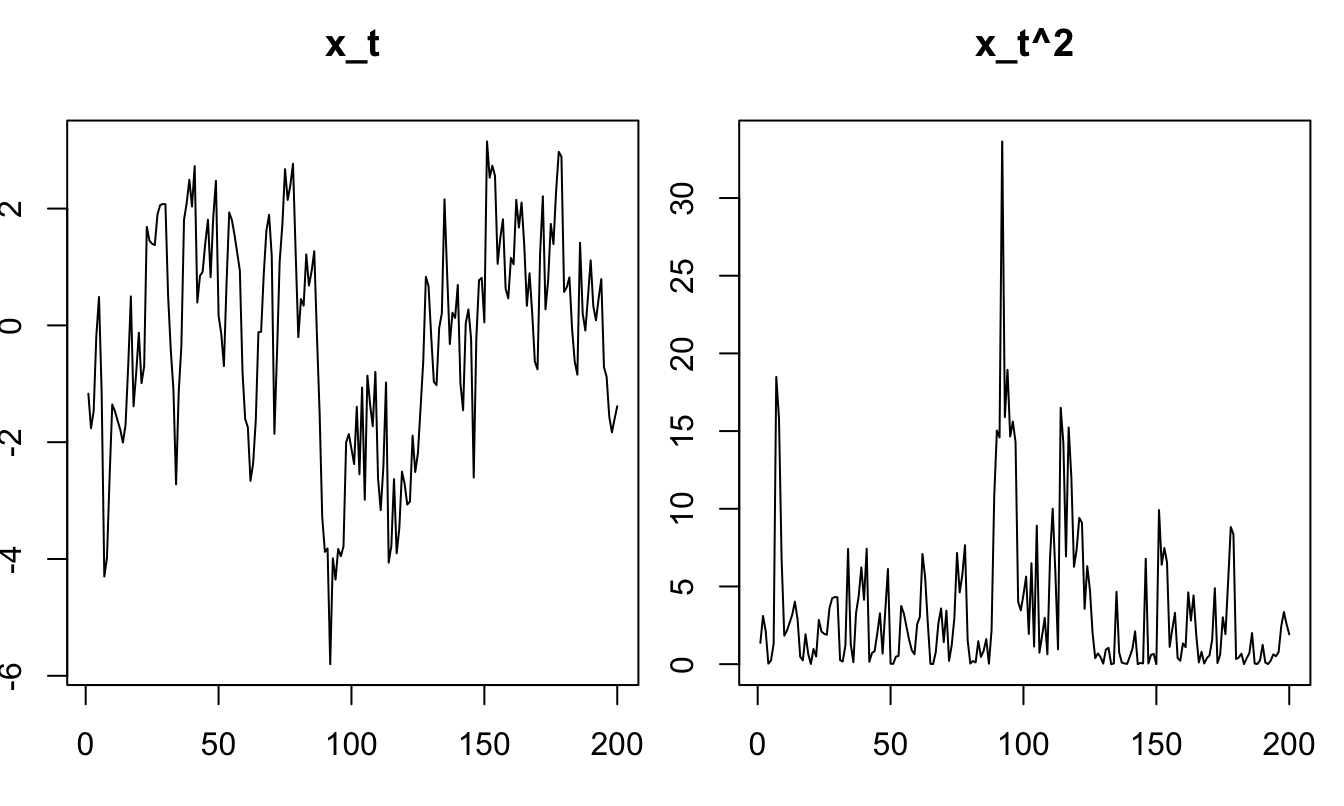
\includegraphics[width=0.95\linewidth]{TSM_files/figure-latex/simQVAR-1} \caption{Simulation of a quadratic processes $x_t$.}\label{fig:simQVAR}
\end{figure}

\end{example}

Another example of nonnegative process is that of the auto-regressive Gamma process \citep{Gourieroux_Jasiak_2006} and its extension \citep{zarg_2017}.

\begin{example}[Autoregressive gamma process, ARG(1)]
\protect\hypertarget{exm:ARG1}{}\label{exm:ARG1}

An ARG process is defined as follows:
\[
\frac{w_{t+1}}{\mu} \sim \gamma(\nu+z_t) \quad \mbox{where} \quad z_t \sim \mathcal{P} \left( \frac{\rho w_t}{\mu} \right),
\]
with \(\nu\), \(\mu\), \(\rho > 0\). (Alternatively \(z_t \sim {\mathcal{P}}(\beta w_t)\), with \(\rho = \beta \mu\).)

Proposition \ref{prp:LTARG} shows that we have \(\varphi_t(u) = \exp[a(u)'w_t+b(u)]\) with
\[
\left\{
\begin{array}{ccc}
a(u) &=&  \dfrac{\rho u}{1-u \mu}\\
b(u) &=& -\nu  
\log(1-u \mu).
\end{array}
\right.
\]

One can simulate ARG processes by using \href{https://jrenne.shinyapps.io/Affine/}{this web-interface} (select the ``ARG'' panel).

It can be shown that:
\[
\left\{
\begin{array}{ccc}
\mathbb{E}(w_{t+1}|\underline{w_t}) &=& \nu \mu + \rho w_t \\
\mathbb{V}ar(w_{t+1}|\underline{w_t}) &=& \nu \mu^2 + 2 \mu \rho w_t.
\end{array}
\right.
\]
and that:
\[
w_{t+1}=\nu\mu+\rho w_t+\varepsilon_{t+1},
\]
where \(\varepsilon_{t+1}\) is a martingale difference \(\Rightarrow\) \(w_{t+1}\) is a weak \(AR(1)\).

\citet{zarg_2017} porpose the extended ARG process and the ARG\(_0\) process. The latter is such that \(\nu = 0\) and \(\beta w_t\) is replaced with \(\alpha + \beta w_t\), i.e.:
\begin{equation}
\frac{w_{t+1}}{\mu} \sim \gamma(z_t),\quad z_t \sim {\mathcal{P}}(\alpha + \beta w_t).\label{eq:ARG0}
\end{equation}
It is easily seen that we then have:
\[
\varphi_t(u) = exp \left[\frac{\beta \mu u}{1-u \mu} w_t + \frac{\alpha \mu u}{1-u \mu}
\right].
\]
The ARG\(_0\) process features a point mass at zero, with conditional probability \(exp(-\alpha - \beta w_t)\). Note that 0 is absorbing if \(\alpha = 0\).

Figure \ref{fig:simARG0} displays the simulated path of an ARG\(_0\) process (since we set \(\nu\) to zero). Note that function \texttt{simul.ARG} is included in the \texttt{TSModels} package.

\begin{Shaded}
\begin{Highlighting}[]
\FunctionTok{library}\NormalTok{(TSModels)}
\NormalTok{W }\OtherTok{\textless{}{-}} \FunctionTok{simul.ARG}\NormalTok{(}\DecValTok{300}\NormalTok{,}\AttributeTok{mu=}\NormalTok{.}\DecValTok{5}\NormalTok{,}\AttributeTok{nu=}\DecValTok{0}\NormalTok{,}\AttributeTok{rho=}\NormalTok{.}\DecValTok{9}\NormalTok{,}\AttributeTok{alpha=}\NormalTok{.}\DecValTok{1}\NormalTok{)}
\FunctionTok{plot}\NormalTok{(W,}\AttributeTok{type=}\StringTok{"l"}\NormalTok{)}
\end{Highlighting}
\end{Shaded}

\begin{figure}
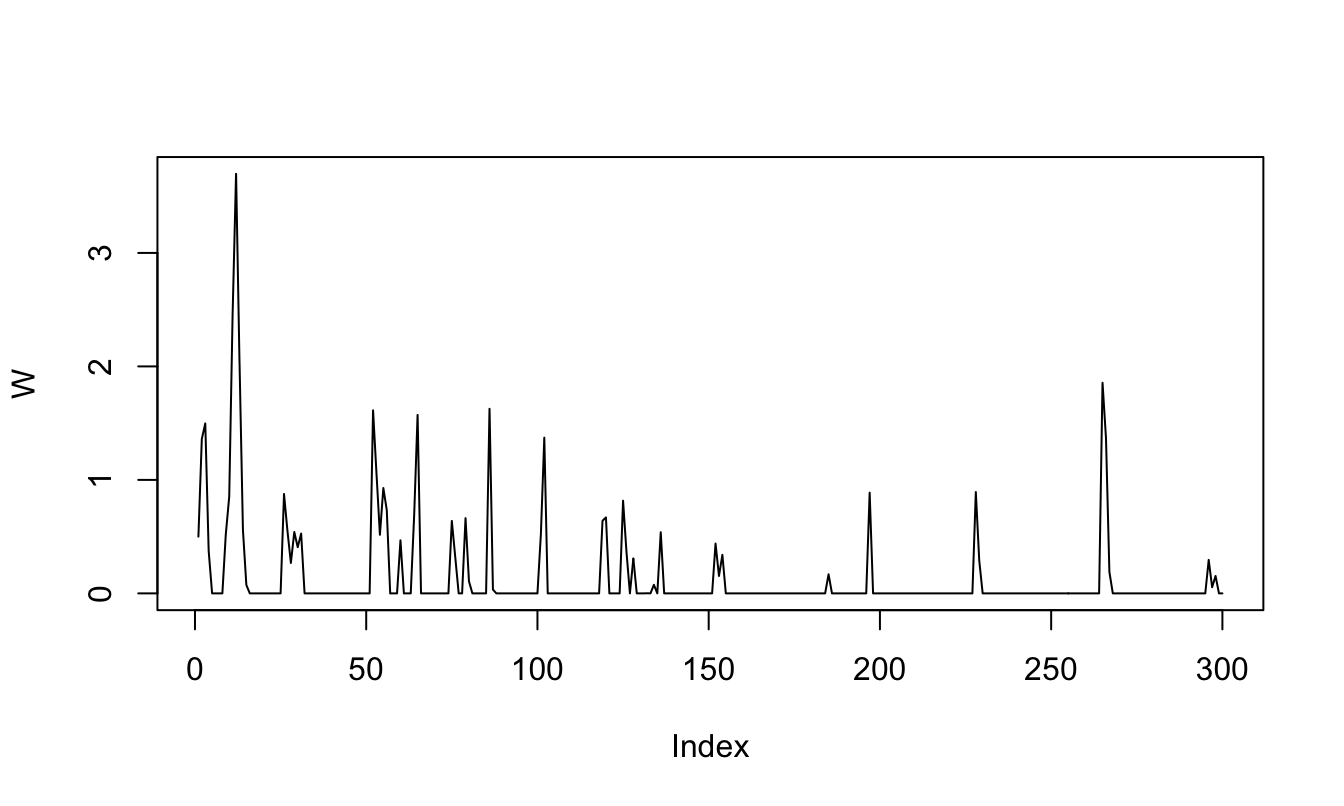
\includegraphics[width=0.95\linewidth]{TSM_files/figure-latex/simARG0-1} \caption{Simulation of an ARG0 processes.}\label{fig:simARG0}
\end{figure}

\end{example}

Certain affine processes are valued in specific sets (e.g., integers). It is the case of compound Poisson proceses:

\begin{example}[Compound Poisson process]
\protect\hypertarget{exm:CompoundPoisson}{}\label{exm:CompoundPoisson}

A compound Poisson process is defined as follows (with \(\gamma > 0\), \(0 < \pi< 1\), and \(\lambda > 0\)):
\[\frac{w_{t+1}}{\gamma} = z_{t+1} + \varepsilon_{t+1},
\]
where \(z_{t+1}\) and \(\varepsilon_{t+1}\) conditionally independent, and where
\(z_{t+1} \sim {\mathcal B} \left(\frac{w_t}{\gamma},\pi\right)\), with \(\varepsilon_{t+1} \sim {\mathcal P}(\lambda)\).

This process is valued in \(\{j \gamma, j \in \mathbb{N}, \gamma \in \mathbb{R}^+\}\) and we have:
\[
\varphi_t(u) = \exp\left\{
\begin{array}{l}
\dfrac{w_t}{\gamma}   \log[\pi
\exp(u\gamma)+1-\pi]-\lambda[1-\exp(u \gamma)]
\end{array}
\right\},
\]
i.e., \(\varphi_t(u) = \exp\left(a(u)w_t+b(u)\right)\) with
\[
\left\{
\begin{array}{ccl}
a(u)&=& \frac{1}{\gamma}   \log[\pi   \exp(u
\gamma)+1-\pi],\\
b(u) &=& -\lambda[1-\exp(u \gamma)].
\end{array}
\right.
\]

We also have: \(w_{t+1} = \pi w_t + \lambda \gamma + \eta_{t+1}\), where \(\eta_{t+1}\) is a
martingale difference.

One can simulate such processes by using \href{https://jrenne.shinyapps.io/Affine/}{this web-interface} (select the ``Compound Poisson'' panel). Figure \ref{fig:simCPoisson} makes use of function \texttt{simul.compound.poisson} (in package \texttt{TSModels}) to simulate a compound Poisson process.

\begin{Shaded}
\begin{Highlighting}[]
\FunctionTok{library}\NormalTok{(TSModels)}
\NormalTok{W }\OtherTok{\textless{}{-}} \FunctionTok{simul.compound.poisson}\NormalTok{(}\DecValTok{100}\NormalTok{,}\AttributeTok{Gamma=}\NormalTok{.}\DecValTok{5}\NormalTok{,}\AttributeTok{Pi=}\FloatTok{0.5}\NormalTok{,}\AttributeTok{lambda=}\NormalTok{.}\DecValTok{9}\NormalTok{)}
\FunctionTok{plot}\NormalTok{(W,}\AttributeTok{type=}\StringTok{"l"}\NormalTok{)}
\end{Highlighting}
\end{Shaded}

\begin{figure}
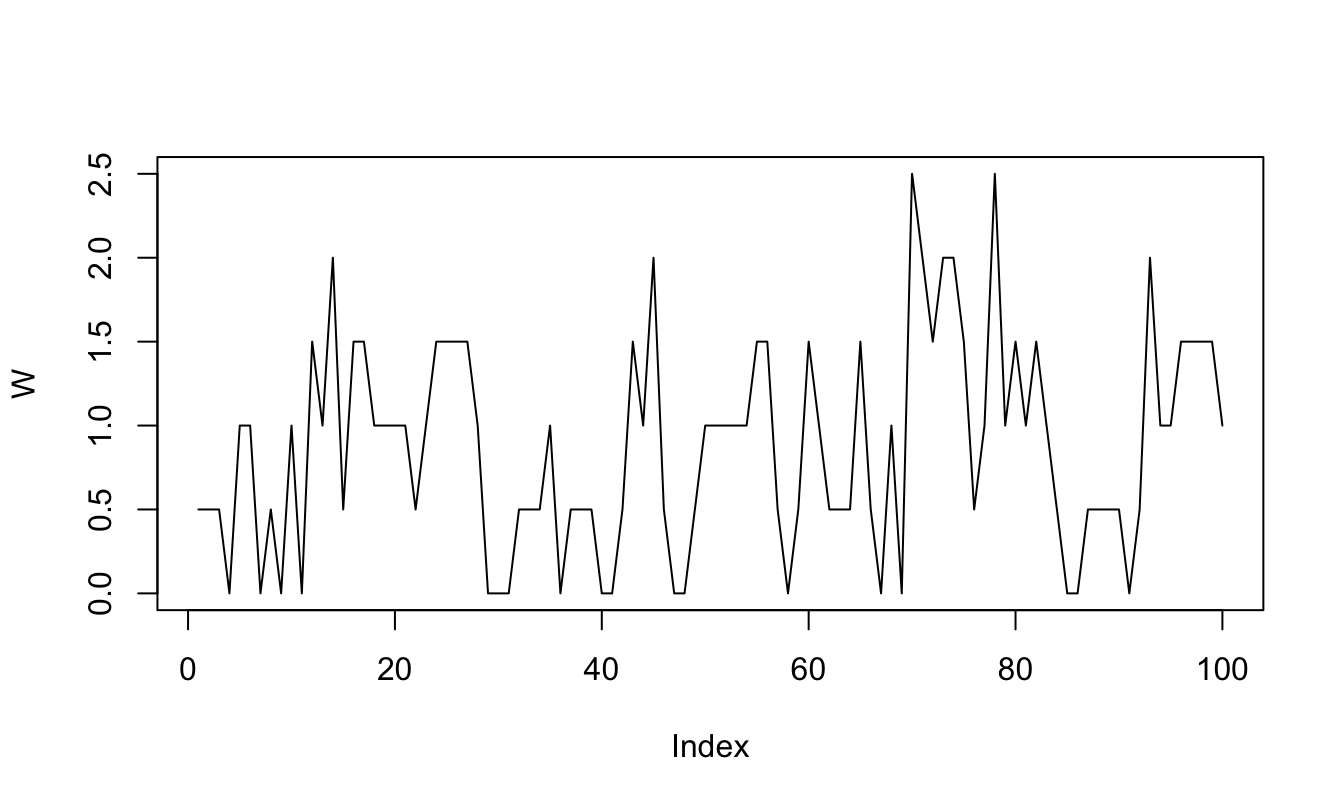
\includegraphics[width=0.95\linewidth]{TSM_files/figure-latex/simCPoisson-1} \caption{Simulation of a Compound Poisson process.}\label{fig:simCPoisson}
\end{figure}

\end{example}

\hypertarget{SubCarp}{%
\subsection{\texorpdfstring{Car processes of order \(p\)}{Car processes of order p}}\label{SubCarp}}

Let us now define Car processes of order \(p\):

\begin{definition}[Affine process of order p]
\protect\hypertarget{def:Carp}{}\label{def:Carp}A multivariate process \(w_{t+1}\) is affine of order \(p\) {[}or \(Car(p)\){]} if there exist functions \(a_1(.),\dots,a_p(.)\), and \(b(.)\) such that:
\[
\varphi_t(u)=\mathbb{E}_t[\exp(u' w_{t+1})]=\exp[a_1(u)'w_t+\dots+a_p(u)'w_{t+1-p}+b(u)].
\]
\end{definition}

It can be seen that if \(w_t\) is \(Car(p)\), then \(W_t = [w_t', w_{t-1}',\dots,w_{t-p+1}']'\) is \(Car(1)\).\footnote{We have:
  \begin{eqnarray*}
  \mathbb{E}_t[\exp(u'W_{t+1})] &=& \mathbb{E}_t[\exp(u'_1 w_{t+1}+u'_2 w_t+\dots+u'_p w_{t-p+2})] \\
  &=& \exp(u'_2 w_t+\dots+u'_p w_{t-p+2})\mathbb{E}_t[\exp(u'_1 w_{t+1})] \\
  &=& \exp(u'_2 w_t+\dots+u'_p w_{t-p+2}+a'_1(u_1)
  w_t  +\dots+a'_p(u_1)w_{t+1-p}+b(u_1)) \\
  &=& \exp[A(u)'W_t+B(u)],
  \end{eqnarray*}
  with \(A(u)' = [u'_2+a'_1(u_1),\dots,u'_p+a'_{p-1}(u_1), a'_p(u_1)]\) and \(B(u) = b(u_1)\).} Therefore, without loss of generality we can assume \(p = 1\).

The standard Car(\(p\)) processes are auto-regressive processes of order \(p\). These processes satisfy the definition of index affine processes:

\begin{definition}[Univariate index affine process of order p]
Let \(\exp[a(u)w_t+b(u)]\) be the conditional Laplace transform of a univariate affine process of order 1, the process \(w_{t+1}\) is an \emph{index-affine} process of order \(p\) if:
\[
\varphi_t(u)=\mathbb{E}_t[\exp(u w_{t+1})]=\exp[a(u)(\beta_1 w_t+\dots+\beta_p
w_{t+1-p})+b(u)].
\]
\end{definition}

Examples \ref{exm:ARp} and \ref{exm:ARGp} are two examples of index affine processes.

\begin{example}[Gaussian AR(p) process]
\protect\hypertarget{exm:ARp}{}\label{exm:ARp}This example extends Example \ref{exm:GAR1}. Consider a Gaussian AR(p) process \(w_t\); that is:
\[
w_{t+1} = \nu + \varphi_1 w_t +\dots+ \varphi_p w_{t+1-p}+\sigma \varepsilon_{t+1},\quad \varepsilon_{t+1} \sim i.i.d. \mathcal{N}(0,1).
\]
We have:
\[
\varphi_t(u) = \exp \left[ u \rho (\beta_1 w_t+\dots+\beta_p w_{t+1-p})+u\nu + u^2  \frac{\sigma^2}{2}\right]
\]
with \(\varphi_i = \rho \beta_i\).
\end{example}

\begin{example}[ARG(p) process (positive)]
\protect\hypertarget{exm:ARGp}{}\label{exm:ARGp}This example extends Example \ref{exm:ARG1}.
An ARG process of order \(p\) is defined as follows:
\[
\frac{w_{t+1}}{\mu} \sim \gamma(\nu+z_t) \quad \mbox{where} \quad z_t \sim \mathcal{P} \left( \beta_1 w_t+\dots+\beta_p w_{t+1-p} \right),
\]
with \(\nu\), \(\mu\), \(\beta_i > 0\). We have:
\[
\varphi_t(u) = \exp\left[\frac{\rho u}{1-u \mu} (\beta_1 w_t+\dots+\beta_p w_{t+1-p})-\nu  \log(1-u\mu)\right],
\]
Process \(w_t\) admits the following AR(\(p\)) representation:
\[
w_{t+1} = \nu\mu + \varphi_1 w_t +\dots+ \varphi_p w_{t+1-p}+\varepsilon_{t+1},
\]
with \(\varphi_i = \beta_i\mu\) and where \(\varepsilon_{t+1}\) is a martingale difference.
\end{example}

\hypertarget{Markov}{%
\section{Markov chains}\label{Markov}}

In this subsection, we show that the family of affine processes includes (some) regime-switching models. We consider a time-homogeneous Markov chain \(z_t\), valued in the set of columns of \(Id_J\), the identity matrix of dimension \(J \times J\). The transition probabilities are denoted by \(\pi(e_i, e_j)\), with \(\pi(e_i, e_j) = \mathbb{P}(z_{t+1}=e_j | z_t=e_i)\). With these notations:
\[
\mathbb{E}[\exp(v'z_{t+1})|z_t=e_i,\underline{z_{t-1}}] = \sum^J_{j=1} \exp(v'e_j)\pi (e_i, e_j).
\]
Hence, we have:
\[
\varphi_t(v) = \exp[a_z(v)'z_t],
\]
with
\[
a_z(v)= \left[ \begin{array}{c} \log \left(\sum^J_{j=1} \exp(v'e_j)  \pi(e_1,e_j)\right)\\
\vdots\\
\log \left(\sum^J_{j=1} \exp(v'e_j)  \pi(e_J,e_j)\right)
\end{array}\right].
\]
This proves that \(z_t\) is an affine process.

One can simulate a two-regime Markov chain by using \href{https://jrenne.shinyapps.io/Affine/}{this web-interface} (select the ``Markov-Switching'' panel).

\hypertarget{WAR}{%
\section{Wishart autoregressive (WAR) processes}\label{WAR}}

WAR are \emph{matrix processes}, valued in the space of \((L \times L)\) symmetric positive
definite matrices.

\begin{definition}[Wishart autoregressive (WAR) processes]
\protect\hypertarget{def:WAR}{}\label{def:WAR}Let \(W_{t+1}\) be a \(WAR_L(K, M, \Omega)\) process. It is defined by:
\begin{eqnarray}
&&\mathbb{E}[\exp   Tr(\Gamma W_{t+1})|\underline{W_t}] \label{eq:Trace}\\
&=& \exp\left\{Tr[M'\Gamma(Id-2\Omega \Gamma)^{-1}M W_t]  -  \frac{K}{2}   \log [det(Id-2\Omega \Gamma)]\right\}, \nonumber
\end{eqnarray}
where \(\Gamma\) is a symmetric matrix,\footnote{Indeed, \(Tr(\Gamma W_{t+1})\) is equal to:
  \begin{eqnarray*}
  \sum^L_{i=1}(\Gamma W_{t+1})_{ii} = \sum^L_{i=1}  \sum^L_{j=1} \gamma_{ij} W_{t+1,ij} = \sum^L_{i=1} \gamma_{ii} W_{t+1,ii} + \sum^L_{i<j} (\gamma_{ij}+\gamma_{ji}) W_{t+1,ij}.
  \end{eqnarray*}} \(K\) is a positive scalar, \(M\) is a \((L \times L)\) matrix, and \(\Omega\) is a \((L \times L)\) symmetric positive definite matrix.
\end{definition}

If \(K\) is an integer, Proposition \ref{prp:WARAR} (in the appendix) shows that \(W_{t+1}\) can be obtained from:
\begin{eqnarray*}
\left\{
\begin{array}{ccl}
W_{t+1} & =&  \sum^K_{k=1} x_{k,t+1} x'_{k,t+1}\\
&&\\
x_{k,t+1} & =& M x_{k,t} + \varepsilon_{k,t+1},\quad k \in \{1,\dots,K\},
\end{array}
\right.
\end{eqnarray*}
where \(\varepsilon_{k,t+1} \sim i.i.d. \mathcal{N}(0, \Omega)\) (independent across \(k\)'s).
The proposition also shows that we have:
\[
\mathbb{E}(W_{t+1}|\underline{W_t}) = MW_tM'+K \Omega,
\]
i.e.~\(W_t\) follows a matrix weak AR(1) process.

In particular case, where \(L=1\) (univariate case), we have that:
\begin{eqnarray*}
\mathbb{E}[\exp(u W_{t+1})|\underline{W_t}] = \exp\left[
\frac{u m^2}{1-2\omega u}W_t -
\frac{K}{2}   \log(1-2\omega u)\right].
\end{eqnarray*}
Hence, when \(L=1\), the Wishart process boils down to an \(ARG(1)\) process (Example \ref{exm:ARG1}) with \(\rho = m^2\), \(\mu = 2\omega\), \(\nu = \frac{K}{2}\).

\hypertarget{building}{%
\section{Building affine processes}\label{building}}

\hypertarget{stoch}{%
\subsection{Univariate affine processes with stochastic parameters}\label{stoch}}

Some univariate affine processes can be extended if they satisfy certain conditions. Specifically, consider a univariate affine process whose conditional L.T. is of the form:
\begin{equation}
\mathbb{E}_t   \exp(u y_{t+1}) = \exp[a_0(u)y_t+b_0(u)\delta],\label{eq:extaffine}
\end{equation}
where \(\delta = (\delta_1,\dots,\delta_m)' \in \mathcal{D}\). This process can be generalized by making \(\delta\) stochastic (while staying in the affine family). More precisely assume that:
\[
\mathbb{E}[\exp(u y_{t+1})|\underline{y_t}, \underline{z_{t+1}}] = \exp[a_0(u)y_t+b_0(u)'\Lambda z_{t+1}],
\]
where \(\Lambda\) is a \((m\times k)\) matrix, with \(\Lambda z_{t+1} \in \mathcal{D}\). In this case, if:
\[
\mathbb{E}[\exp(v' z_{t+1})|\underline{y_t}, \underline{z_{t}}] = \exp[a_1(v)'z_t+b_1(v)],
\]
then \(w_{t+1} = (y_{t+1}, z'_{t+1})'\) is affine.\footnote{Indeed, we have:
  \begin{eqnarray*}
  &&\mathbb{E}[\exp(u y_{t+1}+v'z_{t+1})|\underline{y_t}, \underline{z_{t}}] \\
  &=& \mathbb{E}\{\exp(v' z_{t+1})\mathbb{E}[\exp(u y_{t+1})|\underline{y_t},
  \underline{z_{t+1}}]|\underline{y_t}, \underline{z_{t}} \} \\
  &=& \mathbb{E}\{\exp[a_0(u) y_{t}+b_0(u)'\Lambda z_{t+1}+v'z_{t+1}]|\underline{y_t},
  \underline{z_{t}} \} \\
  &=& \exp\{ a_0(u) y_{t}+a_1[\Lambda' b_0(u)+v]'z_t+b_1 [\Lambda' b_0(u)+v]\}.
  \end{eqnarray*}}

\begin{example}[Gaussian AR(p)]
\protect\hypertarget{exm:extendedARp}{}\label{exm:extendedARp}

Using the notation of Example \ref{exm:ARp}, it comes that an AR(p) processes satisfies Eq. \eqref{eq:extaffine} with \(b_0(u) = \left(u, \; \frac{u^2}{2}\right)'\) and \(\delta = (\nu,\sigma^2)' \in \mathcal{D}=\mathbb{R} \times \mathbb{R}^+\). In that case, \(\delta\) (the vector of conditional mean and variance) can be replaced by \ldots{}

\begin{itemize}
\tightlist
\item
  \(\left( \begin{array}{l} z_{1,t+1} \\ z_{2,t+1} \end{array} \right)\), where \(z_{1,t+1}\) and \(z_{2,t+1}\) are independent AR(1) (see Example \ref{exm:GAR1}) and ARG(1) (see Example \ref{exm:ARG1}) processes, respectively.
\item
  \(\left( \begin{array}{ll} \lambda'_1 & 0 \\ 0 & \lambda'_2 \end{array} \right)\)\(\left( \begin{array}{l} z_{1,t+1} \\ z_{2,t+1} \end{array} \right)\), where \(z_{1,t+1}\) and \(z_{2,t+1}\) are independent Markov chains.
\item
  \(\left( \begin{array}{l} \lambda'_1 \\ \lambda'_2 \end{array}\right)z_{t+1}\), where \(z_{t+1}\) is a Markov chain.
\end{itemize}

\end{example}

\begin{example}[ARG(p) model]
\protect\hypertarget{exm:ARGp}{}\label{exm:ARGp}\leavevmode

\begin{itemize}
\tightlist
\item
  \(b_0(u)= - \nu \log(1-u\mu)\), \(\delta=\nu\).
\item
  \(\nu\) (\(\ge 0\)) can be specified for instance as a Markov chain or an ARG.
\end{itemize}

\end{example}

\hypertarget{buildingmulti}{%
\subsection{Multivariate affine processes}\label{buildingmulti}}

One can construct multivariate affine processes by employing the so-called recursive approach. Let us illustrate this by considering the bivariate case. (The multivariate generalization is straightforward.) Consider \(w_t = \left(\begin{array}{c} w_{1,t}\\ w_{2,t} \end{array} \right)\),and assume that we have:
\begin{eqnarray*}
&&\mathbb{E}[\exp(u_1 w_{1,t+1}|\underline{w_{1,t}}, \underline{w_{2,t}})]\\
&=& \exp[a_{11}(u_1)w_{1,{\color{red}{t}}}+a_{12}(u_1)w_{2,{\color{red}{t}}}+b_{1}(u_1)],
\end{eqnarray*}
and:
\begin{eqnarray*}
&& \mathbb{E}[\exp(u_2 w_{2,t+1}|\underline{w_{1,t+1}}, \underline{w_{2,t}})]\\
&= & \exp[a_0(u_2)w_{1,{\color{red}{t+1}}}+a_{21}(u_2)w_{1,{\color{red}{t}}}+a_{22}(u_2)w_{2,{\color{red}{t}}}+b_2(u_2)].
\end{eqnarray*}
Then \(w_t\) is an affine process.\footnote{Indeed, we have:
  \begin{eqnarray*}
  && \mathbb{E}[\exp(u_1 w_{1,t+1}+u_2 w_{2,t+1}|\underline{w_{1,t}}, \underline{w_{2,t}})]\\
  &= & \mathbb{E}\{\exp(u_1 w_{1,t+1}) \mathbb{E}[\exp(u_{2}w_{2,t+1})|\underline{w_{1,t+1}}, \underline{w_{2,t}})]|\underline{w_{1,t}}, \underline{w_{2,t}})\} \\
  &= & \mathbb{E}\{\exp[u_1+a_0(u_2)w_{1,t+1}+a_{21}(u_2)w_{1,t} + a_{22}(u_2)w_{2,t}+b_2(u_2)]|\underline{w_{1,t}}, \underline{w_{2,t}})\} \\
  &= & \exp\{a_{11}[u_1+a_0(u_2)]w_{1,t}+a_{12}[u_1+a_0(u_2)]w_{2,t}+b_1[u_1+a_0(u_2)] \\
  &&+  a_{21}(u_2)w_{1,t}+a_{22}(u_2)w_{2,t}+b_2(u_2)\}.
  \end{eqnarray*}}
The dynamics of the two components of \(w_t\) are of the form:
\begin{eqnarray*}
w_{1,t+1} &=& \alpha_1 \hspace{1.55cm} + \alpha_{11}w_{1,t} + \alpha_{12}w_{2,t} + \varepsilon_{1,t+1} \\
w_{2,t+1} &=& \alpha_2 + \alpha_{0}w_{1,t+1} + \alpha_{21}w_{1,t} + \alpha _{22} w_{2,t} + \varepsilon_{2,t+1}
\end{eqnarray*}
Note that \(\varepsilon_{1,t+1}\) and \(\varepsilon_{2,t+1}\) are non-correlated martingale differences. In the general case, they are conditionally heteroskedastic. What precedes is at play in \(VAR\) model; \citet{zarg_2017} employ this approach to build vector auto-regressive gamma (VARG) processes.

\hypertarget{extending-multivariate-stochastic-processes}{%
\subsection{Extending multivariate stochastic processes}\label{extending-multivariate-stochastic-processes}}

Consider the same framework as in Section \ref{stoch} when \(y_t\) is a \(n\)-dimensional vector. That is, replace Eq. \eqref{eq:extaffine} with:
\begin{equation}
\mathbb{E}_t   \exp(u' y_{t+1}) = \exp[a_0(u)'y_t+b_0(u)\delta],\label{eq:Multiextaffine}
\end{equation}
and further assume that \(\delta\) is stochastic and depends on \(z_t\), such that:
\[
\mathbb{E}[\exp(u y_{t+1})|\underline{y_t}, \underline{z_{t+1}}] = \exp[a_0(u)y_t+b_0(u)'\Lambda z_{t+1}],
\]
where \(\Lambda\) is a \((m\times k)\) matrix, with \(\Lambda z_{t+1} \in \mathcal{D}\). In this case, if:
\[
\mathbb{E}[\exp(v' z_{t+1})|\underline{y_t}, \underline{z_{t}}] = \exp[a_1(v)'z_t+b_1(v)],
\]
then \(w_{t+1} = (y_{t+1}, z'_{t+1})'\) is affine.

\begin{example}[Stochastic parameters Gaussian VAR(1)]
\protect\hypertarget{exm:RSVAR}{}\label{exm:RSVAR}

This example extends Example \ref{exm:GVAR1}. Using the same notations as in the latter example \ref{exm:GVAR1}, we have
\[
b_0(u) = \left(u', \frac{1}{2} (u \otimes u)'\right)' \quad \mbox{and} \quad\delta = (\mu', vec(\Sigma)')' \in \mathbb{R}^n \times vec(\mathcal{S}),
\]
where \(\mathcal{S}\) is the set of symmetric positive semi-definite matrices. Vector \(\delta\) can be replaced by:
\[
\left( \begin{array}{l} z_{1,t+1}
\\ z_{2,t+1}
\end{array} \right),
\]
where

\begin{itemize}
\tightlist
\item
  \(z_{1,t+1}\) is, for instance, a Gaussian VAR process.
\item
  \(z_{2,t+1}\) is
\item
  obtained by applying the \(vec\) operator to a Wishart process,
\item
  replaced by \(\Lambda_2 z_{2,t+1}\), where \(\Lambda_2\) is a \((n^2 \times J)\) matrix whose columns are \(vec(\Sigma_j)\), \(j \in \{1,\dots,J\}\), the \(\Sigma_j\) being \((n \times n)\) positive semi-definite,
\item
  a standardized \(J\)-dimensional VARG process (multivariate extension of Example \ref{exm:ARG1}).
\end{itemize}

\end{example}

\begin{example}[Regime-switching VAR(1)]
\protect\hypertarget{exm:RSVAR2}{}\label{exm:RSVAR2}

One can also use this approach to construct (affine) regime-switching VAR processes (which is another extension of Example \ref{exm:GVAR1}. For that, replace \(\delta\) with

\begin{itemize}
\tightlist
\item
  \(\left( \begin{array}{ll} \Lambda_1 & 0 \\ 0 & \Lambda_2 \end{array} \right)\)\(\left( \begin{array}{l} z_{1,t+1} \\ z_{2,t+1} \end{array} \right)\), where \(\Lambda_1\) is a \((n \times J_1)\) matrix and \(z_{1,t+1}\) is a Markov chain valued in the set of selection vectors of size \(J_1\) (see Subsection \ref{Markov}), \(\Lambda_2\) is the same matrix as in Example \ref{exm:RSVAR} and \(z_{2,t+1}\) is a Markov chain valued in the set of selection vectors of size \(J_2\).
\item
  or \(\left( \begin{array}{l} \Lambda_1 \\ \Lambda_2 \end{array}\right)z_{t+1}\), where \(\Lambda_1\) and\(\Lambda_2\) are the same matrices as above with \(J_1=J_2=J\), and \(z_{t+1}\) is a Markov chain valued in the set of selection vectors of size \(J\).
\end{itemize}

\end{example}

\hypertarget{AffineExtended}{%
\subsection{Extended affine processes}\label{AffineExtended}}

Some processes are not affine, but may be sub-components of an affine process. This can be useful to compute their conditional moments and multi-horizon Laplace transform (as one can use the formulas presented above for that, using the enlarged---affine---vector).

Let us formally define an extended affine process:

\begin{definition}[Extended Affine Processes]
\protect\hypertarget{def:ExtAffine}{}\label{def:ExtAffine}A process \(w_{1,t}\) is extended affine if there exists a process \(w_{2,t} = g(\underline{w_{1,t}})\) such that \((w'_{1,t}, w'_{2,t})'\) is affine (of order 1).
\end{definition}

For an extended affine processes, \(\varphi_{1,t}(u) = \mathbb{E}[\exp(u'w_{1,t+1})|\underline{w_{1,t}}]\) can be obtained from:
\begin{eqnarray*}
\varphi_t(u_1, u_2) &=& \mathbb{E}[\exp(u'_1w_{1,t+1}+u'_2 w_{2,t+1)}|\underline{w_{1,t}}, \underline{w_{2,t}}] \\
&=& \exp[a'_1(u_1,u_2)w_{1,t} + a'_2(u_1,u_2)w_{2,t}+b(u_1,u_2)]
\end{eqnarray*}
by:
\[
\varphi_{1,t}(u) = \varphi_t(u, 0) = \exp[a'_1(u,0)w_{1,t}+a'_2(u,0)g(\underline{w_{1,t}}) + b(u, 0)].
\]
In particular \(w_{1,t}\) may be non-Markovian.

Similarly the multi-horizon Laplace transform (see Section \ref{MHLT})
\[
\mathbb{E}[\exp(\gamma'_{1}w_{1,t+1}+\dots+\gamma'_{h}w_{1,t+h})|\underline{w_{1,t}}]
\]
can be obtained from the knowledge of the extended multi-horizon Laplace transform:
\begin{eqnarray*}
&&\mathbb{E}_t[\exp(\{\gamma'_{1,1}w_{1,t+1}+\gamma'_{2,1}w_{2,t+1}\}+\dots+ \{\gamma'_{1,h}w_{1,t+h}+\gamma'_{2,h}w_{2,t+h}\}] \\
&=& \exp[A'_{1,t,h}(\gamma^h_1, \gamma^h_2)w_{1,t}+A'_{2,t,h}(\gamma^h_1, \gamma^h_2)w_{2,t}+B_{t,h}(\gamma^h_1, \gamma^h_2)],
\end{eqnarray*}
(with \(\gamma^h_1 = (\gamma'_{1,1},\dots, \gamma'_{1,h})'\), and \(\gamma^h_2 = (\gamma'_{2,1},\dots, \gamma'_{2,h})'\)). We indeed have:
\begin{eqnarray*}
&& \mathbb{E}[\exp(\gamma'_{1}w_{1,t+1}+\dots+\gamma'_{h}w_{1,t+h})|\underline{w_{1,t}}]\\
&=& \exp[A'_{1,t,h}(\gamma^h,0) w_{1,t} + A'_{2,t,h}(\gamma^h,0)g (\underline{w_{1,t}}) + B_{t,h}(\gamma^h,0)],
\end{eqnarray*}
with \(\gamma^h = (\gamma_1',\dots,\gamma_h')'\).

\begin{example}[Affine process of order p]
\protect\hypertarget{exm:AffProcessOrderp}{}\label{exm:AffProcessOrderp}If \(\{w_{1,t}\}\) is affine or order \(p>1\), then \((w_{1,t},\dots,w_{1,t-p+1})\) is affine of order 1, but \(\{w_{1,t}\}\) is not affine. That is, in that case, \(w_{2,t} = (w'_{1,t-1}, \dots.w'_{1,t-p+1})'\).

This a kind of extreme case since \(w_{2,t}\) belongs to the information at \(t-1\), which implies \(a_2(u_1, u_2) = u_2\).
\end{example}

\begin{example}[Gaussian ARMA process]
\protect\hypertarget{exm:GaussianARMA}{}\label{exm:GaussianARMA}Consider an \(ARMA(1,1)\) process
\[
w_{1,t} - \varphi w_{1,t-1} = \varepsilon_t-\theta \varepsilon_{t-1},
\]
with \(|\varphi | < 1\), \(|\theta| < 1\), and \(\varepsilon_t \sim i.i.d. \mathcal{N}(0, \sigma^2)\).

\(w_{1,t}\) is not Markovian. Now, take \(w_{2,t} = \varepsilon_t = (1-\theta L)^{-1}(1-\varphi L)w_{1,t}\). We have:
\[
\left(
\begin{array}{l}
w_{1,t+1} \\
w_{2,t+1}
\end{array}
\right) =
\left(
\begin{array}{ll}
\varphi & -\theta \\
0 &      0
\end{array}
\right)
\left(
\begin{array}{l}
w_{1,t} \\
w_{2,t}
\end{array}
\right) +
\left(
\begin{array}{l}
1 \\
1
\end{array}
\right) \varepsilon_{t+1}.
\]
Hence \((w_{1,t}, w_{2,t})'\) is Gaussian \(VAR(1)\), and, therefore, it is affine of order 1.

This is easily extended to \(ARMA(p,q)\) and \(VARMA(p,q)\) processes.
\end{example}

\begin{example}[GARCH type process]
\protect\hypertarget{exm:GARCH}{}\label{exm:GARCH}Consider process \(w_{1,t}\), defined by:
\[
w_{1,t+1}  = \mu + \varphi w_{1,t} + \sigma_{t+1} \varepsilon_{t+1},
\]
where \(|\varphi| < 1\) and \(\varepsilon_t \sim i.i.d. \mathcal{N}(0,1)\), and
\[
\sigma^2_{t+1} = \omega + \alpha \varepsilon^2_t + \beta \sigma^2_t,
\]
where \(0 < \beta < 1\).

Consider \(w_{2,t} = \sigma^2_{t+1}\) (which is a non-linear function of \(\underline{w_{1,t}}\)). Proposition \ref{prp:GARCH} shows that:
\begin{eqnarray*}
&& \mathbb{E}\left[\exp(u_1 w_{1,t+1} + u_2 w_{2,t+1})|\underline{w_{1,t}}\right] \\
&=& \exp\left[u_1 \mu + u_2 \omega - \frac{1}{2}   \log(1-2 u_2 \alpha) \right. \\
&&\left. +  u_1 \varphi w_{1,t} + (u_2\beta +  \frac{u^2_1}{2(1-2u_2\alpha)}) w_{2,t}\right],
\end{eqnarray*}
which is exponential affine in \((w_{1,t}, w_{2,t})\).
\end{example}

\hypertarget{MHLT}{%
\section{Multi-horizon Laplace transform}\label{MHLT}}

\hypertarget{recursive-computation-and-direct-pricing-implications}{%
\subsection{Recursive computation and direct pricing implications}\label{recursive-computation-and-direct-pricing-implications}}

In this subsection, we show that multi-horizon Laplace transforms of affine processes can be calculated recursively. Various examples will show how this can be exploited to price long-dated financial instruments.

Let us consider a multivariate process \(w_{t}\), affine of order one. (As explained in Subsection \ref{SubCarp}, this includes the case of the order \(p\) case.) For the sake of generality, we consider the case where functions \(a(.)\), \(b(.)\) are possibly deterministic functions of time, denoted in this case \(a_{t+1}(.)\) and \(b_{t+1}(.)\):
\[
\mathbb{E}_t \exp[(u'w_{t+1})] = \exp[a'_{t+1}(u)w_t+b_{t+1}(u)].
\]
The multi-horizon Laplace transform of associated with date \(t\) and horizon \(h\) is defined by:
\begin{equation}
\varphi_{t,h}(\gamma_1,\dots,\gamma_h) = \mathbb{E}_t[\exp(\gamma'_1w_{t+1}+\dots+\gamma'_h w_{t+h})].\label{eq:multiLT}
\end{equation}

Lemma \ref{lem:MHLT} (in the appendix) shows that we have:
\[
\varphi_{t,h}(\gamma_1,\dots,\gamma_h) = \exp(A'_{t,h} w_t + B_{t,h}),
\]
where \(A_{t,h} = A^h_{t,h}\) and \(B_{t,h} = B^h_{t,h}\), the \(A^h_{t,i}, B^h_{t,i}\) \(i = 1,\dots,h\), being given recursively by:
\[
\left\{
\begin{array}{ccl}
A^h_{t,i} &=& a_{t+h+1-i}(\gamma_{h+1-i} + A^h_{t,i-1}), \\
B^h_{t,i} &=& b_{t+h+1-i}(\gamma_{h+1-i} + A^h_{t,i-1}) + B^h_{t,i-1}, \\
A^h_{t,0} &=& 0, B^h_{t,0} = 0.
\end{array}
\right.
\]

If the functions \(a_{t}\) and \(b_{t}\) do not depend on \(t\), these recursive formulas do not depend on \(t\), and we get \(\varphi_{t,h}(\gamma_1,\dots,\gamma_h)\), for any \(t\), with only one recursion for each \(h\).

Moreover, if the functions \(a_{t}\) and \(b_{t}\) do not depend on \(t\), and if different sequences \((\gamma^h_1,\dots,\gamma^h_h), h=1,\dots,H\) (say) satisfy \(\gamma^h_{h+1-i} = u_i\), for
\(i=1,\dots,h\), and for any \(h \leq H\), that is if we want to compute (\emph{reverse-order} case):
\begin{equation}
\varphi_{t,h}(u_h,\dots,u_1)=\mathbb{E}_t[\exp(u'_{{\color{red}h}} w_{{\color{red}t+1}}+\dots+u'_{{\color{red}1}} w_{{\color{red}t+h}})],
\quad h=1,\dots,H,\label{eq:LTreverse}
\end{equation}
then Proposition \ref{prp:reverseMLT} (in the appendix) shows that we can compute the \(\varphi_{t,h}(u_h,\dots,u_1)\) for any \(t\) and any \(h \leq H\) with only one recursion. That is \(\varphi_{t,h}(u_h,\dots,u_1)=\exp(A'_hw_t+B_h)\) with:
\begin{equation*}
\left\{
\begin{array}{ccl}
A_{h} &=& a(u_{h} + A_{h-1}), \\
B_{h} &=& b(u_{h} + A_{h-1}) + B_{h-1}, \\
A_{0} &=& 0,\quad  B_{0} = 0.
\end{array}
\right.
\end{equation*}

As mentioned above, what precedes has useful implications to price long-dated financial instruments such as nominal and real bonds (Examples \ref{exm:nominalBth} and \ref{exm:realBth}, respectively), or futures (Example \ref{exm:Futures}).

\begin{example}[Nominal interest rates]
\protect\hypertarget{exm:nominalBth}{}\label{exm:nominalBth}Let \(B(t,h)\) denote the date-\(t\) price of a nominal zero-coupon bond of maturity \(h\). We Have:
\begin{equation}
B(t,h) = \mathbb{E}^{\mathbb{Q}}_t exp (-r_{t}-\dots-r_{t+h-1}),\label{eq:stdbond}
\end{equation}
where \(r_{t}\) is the nominal short rate between \(t\) and \(t+1\) (observed at \(t\)), and the associated (continuously-compounded) yield-to-maturity is given by:
\begin{equation}
R(t,h) = -  \frac{1}{h}   \log   B(t,h), \quad   h=1,\dots,H.
\end{equation}
If \(r_t = \omega'w_t\) (say), then:
\[
B(t,h) = \exp(-r_{t}) \mathbb{E}^{\mathbb{Q}}_t \exp(-\omega' w_{t+1} - \dots - \omega' w_{t+h-1}).
\]
One can then price this bond by directly employing Eq. \eqref{eq:LTreverse}, with \(u_1 = 0\) and \(u_i = - \omega\), \(i = 2,\dots, H\).
The price \(B(t,h)\) is exponential affine in \(w_t\), the associated yield-to-maturity \(R(t,h)=-1/h\log B(t,h)\) is affine in \(w_t\).
\end{example}

\begin{example}[No-arbitrage Nelson-Siegel model]
\protect\hypertarget{exm:CDR2009}{}\label{exm:CDR2009}

In this example, we employ the results of Example \ref{exm:nominalBth} in the context described by \citet{Christensen_Diebold_Rudebusch_2009}. Specifically, we consider a three factor model following a Gaussian VAR (see Example \ref{exm:GVAR1}):
\[
w_t = \left[\begin{array}{c}X_{1,t}\\X_{2,t}\\X_{3,t}\end{array}\right] = 
\left[\begin{array}{ccc}
1 & 0 & 0\\
0&1-\lambda&\lambda\\
0&0&1-\lambda\end{array}\right]
\left[\begin{array}{c}X_{1,t-1}\\X_{2,t-1}\\X_{2,t-1}\end{array}\right] +
\left[\begin{array}{ccc}
\sigma_{11} & 0 & 0\\
\sigma_{21}&\sigma_{22}&0\\
\sigma_{31}&\sigma_{32}&\sigma_{33}\end{array}\right]
\left[\begin{array}{c}\varepsilon_{1,t}\\\varepsilon_{2,t}\\\varepsilon_{3,t}\end{array}\right],
\]
where \(\left[\begin{array}{c}\varepsilon_{1,t}\\\varepsilon_{2,t}\\\varepsilon_{3,t}\end{array}\right] \sim \,i.i.d.\, \mathcal{N}(0,Id)\).

The nominal short-term rate is given by \(r_t = X_{1,t}+X_{2,t}\). In that case, we can use the results of Example \ref{exm:nominalBth} with \(\omega = (-1,-1,0)'\). The following lines of code do that:

\begin{Shaded}
\begin{Highlighting}[]
\FunctionTok{library}\NormalTok{(TSModels)}
\NormalTok{lambda }\OtherTok{\textless{}{-}}\NormalTok{ .}\DecValTok{05}
\NormalTok{Phi }\OtherTok{\textless{}{-}} \FunctionTok{diag}\NormalTok{(}\FunctionTok{c}\NormalTok{(}\DecValTok{1}\NormalTok{,}\DecValTok{1}\SpecialCharTok{{-}}\NormalTok{lambda,}\DecValTok{1}\SpecialCharTok{{-}}\NormalTok{lambda));Phi[}\DecValTok{2}\NormalTok{,}\DecValTok{3}\NormalTok{] }\OtherTok{\textless{}{-}}\NormalTok{ lambda}
\NormalTok{Sigma }\OtherTok{\textless{}{-}}\NormalTok{ .}\DecValTok{0005} \SpecialCharTok{*} \FunctionTok{diag}\NormalTok{(}\DecValTok{3}\NormalTok{)}
\NormalTok{psi.parameterization}\OtherTok{=}\FunctionTok{list}\NormalTok{(}\AttributeTok{mu=}\FunctionTok{matrix}\NormalTok{(}\DecValTok{0}\NormalTok{,}\DecValTok{3}\NormalTok{,}\DecValTok{1}\NormalTok{),}\AttributeTok{Phi=}\NormalTok{Phi,}\AttributeTok{Sigma=}\NormalTok{Sigma)}
\NormalTok{u1 }\OtherTok{\textless{}{-}} \FunctionTok{matrix}\NormalTok{(}\DecValTok{0}\NormalTok{,}\DecValTok{3}\NormalTok{,}\DecValTok{1}\NormalTok{)}
\NormalTok{u2 }\OtherTok{\textless{}{-}} \FunctionTok{matrix}\NormalTok{(}\FunctionTok{c}\NormalTok{(}\SpecialCharTok{{-}}\DecValTok{1}\NormalTok{,}\SpecialCharTok{{-}}\DecValTok{1}\NormalTok{,}\DecValTok{0}\NormalTok{),}\AttributeTok{ncol=}\DecValTok{1}\NormalTok{)}
\NormalTok{H }\OtherTok{\textless{}{-}} \DecValTok{20}
\NormalTok{AB }\OtherTok{\textless{}{-}} \FunctionTok{reverse.MHLT}\NormalTok{(psi.GaussianVAR,}\AttributeTok{u1 =}\NormalTok{ u1,}\AttributeTok{u2 =}\NormalTok{ u2,}\AttributeTok{H =}\NormalTok{ H,}
                   \AttributeTok{psi.parameterization =}\NormalTok{ psi.parameterization)}
\NormalTok{AB}\SpecialCharTok{$}\NormalTok{A[}\DecValTok{1}\SpecialCharTok{:}\DecValTok{2}\NormalTok{,,] }\OtherTok{\textless{}{-}}\NormalTok{ AB}\SpecialCharTok{$}\NormalTok{A[}\DecValTok{1}\SpecialCharTok{:}\DecValTok{2}\NormalTok{,,] }\SpecialCharTok{{-}} \DecValTok{1} \CommentTok{\# add terms corresponding to exp({-}r\_t)}
\NormalTok{a.yield }\OtherTok{\textless{}{-}} \SpecialCharTok{{-}}\NormalTok{ AB}\SpecialCharTok{$}\NormalTok{A }\SpecialCharTok{/} \FunctionTok{array}\NormalTok{((}\DecValTok{1}\SpecialCharTok{:}\NormalTok{H) }\SpecialCharTok{\%x\%} \FunctionTok{rep}\NormalTok{(}\DecValTok{1}\NormalTok{,}\DecValTok{3}\NormalTok{),}\FunctionTok{c}\NormalTok{(}\DecValTok{3}\NormalTok{,}\DecValTok{1}\NormalTok{,H))}
\NormalTok{b.yield }\OtherTok{\textless{}{-}} \SpecialCharTok{{-}}\NormalTok{ AB}\SpecialCharTok{$}\NormalTok{B }\SpecialCharTok{/} \FunctionTok{array}\NormalTok{((}\DecValTok{1}\SpecialCharTok{:}\NormalTok{H) }\SpecialCharTok{\%x\%} \FunctionTok{rep}\NormalTok{(}\DecValTok{1}\NormalTok{,}\DecValTok{3}\NormalTok{),}\FunctionTok{c}\NormalTok{(}\DecValTok{1}\NormalTok{,}\DecValTok{1}\NormalTok{,H))}
\FunctionTok{plot}\NormalTok{(a.yield[}\DecValTok{1}\NormalTok{,,],}\AttributeTok{type=}\StringTok{"l"}\NormalTok{,}\AttributeTok{lwd=}\DecValTok{2}\NormalTok{,}\AttributeTok{ylim=}\FunctionTok{c}\NormalTok{(}\DecValTok{0}\NormalTok{,}\DecValTok{1}\NormalTok{),}
     \AttributeTok{xlab=}\StringTok{"Maturity"}\NormalTok{,}\AttributeTok{ylab=}\StringTok{"Factor loadings"}\NormalTok{)}
\FunctionTok{lines}\NormalTok{(a.yield[}\DecValTok{2}\NormalTok{,,],}\AttributeTok{col=}\StringTok{"red"}\NormalTok{,}\AttributeTok{lwd=}\DecValTok{2}\NormalTok{,}\AttributeTok{lty=}\DecValTok{2}\NormalTok{)}
\FunctionTok{lines}\NormalTok{(a.yield[}\DecValTok{3}\NormalTok{,,],}\AttributeTok{col=}\StringTok{"blue"}\NormalTok{,}\AttributeTok{lwd=}\DecValTok{2}\NormalTok{,}\AttributeTok{lty=}\DecValTok{3}\NormalTok{)}
\end{Highlighting}
\end{Shaded}

\begin{figure}
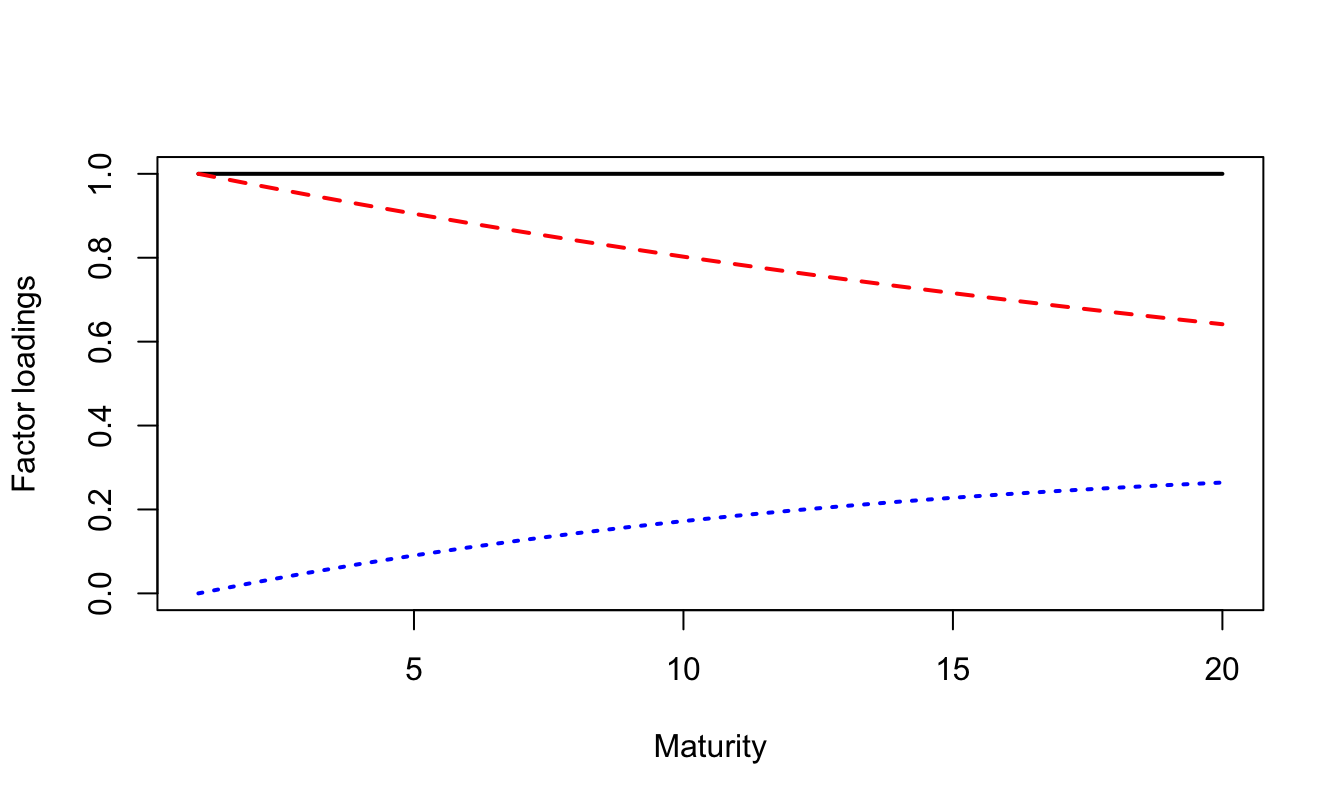
\includegraphics[width=0.95\linewidth]{TSM_files/figure-latex/CDR-1} \caption{Factor loadings in the context of a no-arbitrage nelson-Siegel model (Christensen, Diebold and Rudebusch, 2009). The first factor (black solid line) is a level factor. The second and third factors (red dashed line and blue dotted line, respectively) are slope factors.}\label{fig:CDR}
\end{figure}

\end{example}

In the previous example, note the use of function \texttt{reverse.MHLT} (in package \texttt{TSModels}), that notably takes a L.T. as an argument (\texttt{psi}). In the previous example, we consider a Gaussian VAR, and we therefore assign \texttt{psi.GaussianVAR} to \texttt{psi}. We then need to provide function \texttt{reverse.MHLT} with the arguments of the \texttt{psi} function. These arguments are provided in the form of a list (input \texttt{psi.parameterization}).

\begin{example}[Real interest rates]
\protect\hypertarget{exm:realBth}{}\label{exm:realBth}Denote by \(q_t\) the price index on date \(t\) and by \(\pi_{t+1} = \log \dfrac{q_{t+1}}{q_t}\) the inflation rate on date \(t+1\). We have:
\begin{eqnarray*}
\bar{R}(t,h) & =& -   \frac{1}{h}   \log   \bar{B}(t,h), \quad h=1,\dots,H \\    \\
\bar{B}(t,h) & =&  \mathbb{E}^{\mathbb{Q}}_t   \exp(-r_{t}-\dots-r_{t+h-1} + \pi_{t+1}+\dots+\pi_{t+h}),  \\      \\
& =& \exp(-r_{t}) \times \\
&& \mathbb{E}^{\mathbb{Q}}_t \exp(-r_{t+1}-\dots-r_{t+h-1}+\pi_{t+1}+\dots+\pi_{t+h})
\end{eqnarray*}
If \(r_t = \omega'w_t\) and \(\pi_t = \bar\omega'w_t\), then \(\bar{B}(t,h)\) is given by:
\begin{eqnarray*}
\exp(-r_{t}) \mathbb{E}^{\mathbb{Q}}_t exp[(\bar\omega-\omega)'w_{t+1}+\dots+(\bar\omega-\omega)'w_{t+h-1}+\bar\omega'
w_{t+h}]
\end{eqnarray*}
One can then price this bond by directly employing Eq. \eqref{eq:LTreverse}, with \(u_1 = \bar\omega\) and \(u_i = \bar\omega-\omega\), \(i = 2,\dots, H\).
\end{example}

\begin{example}[Futures]
\protect\hypertarget{exm:Futures}{}\label{exm:Futures}

Denote by \(F(t,h)\) the date-\(t\) price of a future of maturity \(h\) (see Section XXX). That is \(F(t,h) = \mathbb{E}^{\mathbb{Q}}_t (S_{t+h})\), \(h=1,\dots,H\), where \(S_t\) is the date-\(t\) price of the underlying asset.

\begin{itemize}
\item
  If \(w_t = (\log S_t, x'_t)'\) then \(F(t,h) = \mathbb{E}^{\mathbb{Q}}_t \exp(e'_1 w_{t+h})\). This can be calculated by using Eq. \eqref{eq:LTreverse} with \(u_1 = e_1\), and \(u_i = 0\), for \(i=2,\dots,H\).
\item
  If \(w_t = (y_t, x'_t)'\) with \(y_t = \log\frac{S_t}{S_{t-1}}\), then \(F(t,h) = S_t \mathbb{E}^{\mathbb{Q}}_t \exp(e'_1 w_{t+1}+\dots+e'_1 w_{t+h})\). This can be calculated by using Eq. \eqref{eq:LTreverse} with \(u_i = e'_1\), \(i=1,\dots,H\).
\end{itemize}

\end{example}

\hypertarget{ExponentialPayoff}{%
\subsection{Exponential payoff}\label{ExponentialPayoff}}

Consider an asset providing the payoff \(\exp(\nu' w_{t+h})\) on date \(t+h\). Its price is given by:
\[
P(t,h;\nu) = \mathbb{E}^{\mathbb{Q}}_t[\exp(-r_{t}-\dots-r_{t+h-1}) \exp(\nu' w_{t+h})].
\]
If \(r_t = \omega'w_t\), we have:
\[
P(t,h;\nu) = \exp(-r_{t})\mathbb{E}^{\mathbb{Q}}_t \left(exp[-\omega' w_{t+1}-\dots-\omega' w_{t+h-1}+ \nu' w_{t+h}]\right),
\]
which can be calculated by Eq. \eqref{eq:LTreverse}, with \(u_1 = \nu\) and \(u_i = -\omega\) for \(i = 2,\dots,H\).

What precedes can be extended to the case where the payoff (settled on date \(t+h\)) is of the form:
\[
(\nu_1'w_{t+h}) \exp(\nu_2' w_{t+h}).
\]
Indeed, we have
\[
\left[\frac{\partial \exp[(s \nu_1+ \nu_2)'w_{t+h}]}{\partial s}\right]_{s=0} = (\nu_1'w_{t+h}) \exp(\nu_2' w_{t+h}).
\]
Therefore:
\begin{eqnarray}
&&\mathbb{E}_t^{\mathbb{Q}}[\exp(-r_t - \dots - r_{t+h-1})(\nu_1'w_{t+h}) \exp(\nu_2' w_{t+h})] \nonumber\\
&=& \left[
\frac{\partial P(t,h;s \nu_1 + \nu_2)}{\partial s}
\right]_{s=0}.\label{eq:Affineexppayoff}
\end{eqnarray}
This method is easily extended to price payoffs of the form \((\nu_1'w_{t+h})^k \exp(\nu_2' w_{t+h})\), with \(k \in \mathbb{N}\).

\hypertarget{var-representation-and-conditional-moments}{%
\section{VAR representation and conditional moments}\label{var-representation-and-conditional-moments}}

An important property of affine processes is that their dynamics can be written as a vector-autoregressive process. This is useful to compute conditional moments of the process.

\begin{proposition}[VAR representation of an affine process' dynamics]
\protect\hypertarget{prp:affineVAR}{}\label{prp:affineVAR}If \(w_t\) is the affine process whose Laplace transform is defined in Def. \ref{def:Car1}, then its dynamics admits the following vectorial autoregressive representation:
\begin{equation}
w_{t+1} = \mu + \Phi w_{t} + \Sigma^{\frac{1}{2}}(w_t) \varepsilon_{t+1},\label{eq:VARw}
\end{equation}
where \(\varepsilon_{t+1}\) is a difference of martingale sequence whose conditional covariance matrix is the identity matrix and where \(\mu\), \(\Phi\) and \(\Sigma(w_t) = \Sigma^{\frac{1}{2}}(w_t){\Sigma^{\frac{1}{2}}(w_t)}'\) satisfy:
\begin{equation}
\mu =  \left[\frac{\partial }{\partial u}b(u)\right]_{u=0}, \quad \Phi= \left[\frac{\partial }{\partial u}a(u)'\right]_{u=0}\label{eq:MUPHI}
\end{equation}
\begin{equation}
\Sigma(w_t) =  \left[\frac{\partial }{\partial u\partial u'}b(u)\right]_{u=0} + \left[\frac{\partial }{\partial u\partial u'}a(u)'w_t\right]_{u=0}.\label{eq:SigmaWt}
\end{equation}
\end{proposition}

\begin{proof}
When \(w_t\) is affine, its (conditional) cumulant generating function is of the form \(\psi(u)=a(u)'w_t+b(u)\). The result directly follows from the formulas given in Section \ref{AffineLaplace}.
\end{proof}

Proposition \ref{prp:condvarAffine} (in the appendix) shows that the conditional means and variances of \(w_t\) are given by:
\begin{eqnarray}
\mathbb{E}_t(w_{t+h}) &=& (I - \Phi)^{-1}(I - \Phi^h)\mu + \Phi^h w_t \label{eq:condmean}\\
\mathbb{V}ar_t(w_{t+h}) &=& \Sigma(\mathbb{E}_t(w_{t+h-1}))+\Phi \Sigma(\mathbb{E}_t(w_{t+h-2}))\Phi' + \nonumber \\
&& \dots + \Phi^{h-1} \Sigma(w_{t}){\Phi^{h-1}}'. \label{eq:condvar}
\end{eqnarray}
Eq. \eqref{eq:condvar} notably implies that \(\mathbb{V}ar_t(w_{t+h})\) is an affine function of \(w_t\). Indeed \(\Sigma(.)\) is an affine function, and the conditional expectations \(\mathbb{E}_t(w_{t+h})\) are affine in \(w_t\), as shown by Eq. \eqref{eq:condmean}.

The unconditional means and variances are given by:
\begin{equation}
\left\{
\begin{array}{ccl}
\mathbb{E}(w_t) &=& (I - \Phi)^{-1}\mu\\
vec[\mathbb{V}ar(w_t)] &=& (I_{n^2} - \Phi \otimes \Phi)^{-1} vec\left(\Sigma[(I - \Phi)^{-1}\mu]\right).
\end{array}
\right.\label{eq:uncondmeanvar}
\end{equation}

\hypertarget{TransfAna}{%
\section{Truncated Laplace transforms of affine processes}\label{TransfAna}}

In this section, we show how one can employ Fourier transforms to compute truncated conditional moments of affine processes. For that, let us introduce the following notation:
\[
w_{t+1,T} = (w'_{t+1}, w'_{t+2},\dots, w'_T)'
\]
with \(w_t\) affine \(n\)-dimensional process.

We want to compute:
\[
\tilde{\varphi}_t(u ; v, \gamma) = \mathbb{E}_t[\exp(u'w_{t+1,T})\textbf{1}_{\{v'w_{t+1,T}<\gamma\}}].
\]

Consider the complex untruncated conditional Laplace transform:
\[
\varphi_t(z) = \mathbb{E}_t[\exp(z'w_{t+1,T})],\quad  z \in \mathbb{C}^{nT},
\]
computed using the same recursive algorithm as in the real case (see Section \ref{MHLT}).

\citet{Duffie_Pan_Singleton_2000} have shown that we have (see also Proposition \ref{prp:Fourier} in the appendix):
\begin{equation}
\tilde{\varphi}_t(u ; v, \gamma) =  \frac{\varphi_t(u)}{2} - \frac{1}{\pi}
\int^\infty_0 \frac{Im[\varphi_t(u+ivx) \exp(-i\gamma x)]}{x} dx.\label{eq:DPS}
\end{equation}
where \(Im\) means imaginary part.

Note that the integral in Eq. \eqref{eq:DPS} is one dimensional (whatever the dimension of \(w_t\)). As shown in the following example, this can be exploited to price options.

\begin{example}[Option pricing]
\protect\hypertarget{exm:OptionPricing}{}\label{exm:OptionPricing}Pricing calls and puts amounts to conditional expectations of the type (with \(k > 0\)):
\begin{eqnarray*}
&& \mathbb{E}_t\left([\exp(u'_1 w_{t+1,T})-k   \exp(u'_2 w_{t+1,T})]^+\right) \\
&= &  \mathbb{E}_t\left([\exp(u'_1 w_{t+1,T})-k   \exp(u'_2 w_{t+1,T})]\textbf{1}_{\{[\exp(u_1-u_2)'w_{t+1,T}] > k \}}\right) \\
&= & \tilde{\varphi}_t(u_1 ; u_2-u_1, - \log   k) - k \tilde{\varphi}_t(u_2 ; u_2-u_1, - \log   k).
\end{eqnarray*}
\end{example}

\begin{example}[Exogenous short rate]
\protect\hypertarget{exm:ExogSTR}{}\label{exm:ExogSTR}Consider an asset whose date-\(t\) price is \(p_t\). Denote its geometric asset return by \(y_t\), i.e., \(y_t = \log(p_t/p_{t-1})\). Consider an option written on this asset, with a strike equal \(k p_t\).

If interest rates are deterministic, the option price, for a maturity \(h\), is given by:
\[
p_t   \exp(-r_{t}-\dots-r_{t+h-1}) \mathbb{E}^{\mathbb{Q}}_t[\exp   u'_1 w_{t+1, t+h} - k]^+
\]
with \(u_1 = e \otimes e_1\), where \(e\) is the \(h\)-dimensional vector with components equal to 1, and \(e_1\) is the \(n\)-vector selecting the 1st component (\(y_t\) being the 1st component of \(w_t\), say).
\end{example}

\begin{example}[Endogenous short rate]
\protect\hypertarget{exm:EndogSTR}{}\label{exm:EndogSTR}Consider the same context as in Example \ref{exm:ExogSTR}, but with a stochastic (endogenous) short-term rate. For instance, assume that \(r_{t+1} = \omega_0 + \omega'_1 w_t\). The option price then is:
\begin{eqnarray*}
&& p_t \mathbb{E}^{\mathbb{Q}}_t  \left[ \exp(-\omega_0 - \omega'_1 w_t-\dots- \omega_0 - \omega'_1 w_{t+h-1}) [\exp(u'_1 w_{t+1,t+h})-k]^+ \right]\\
&= & p_t   \exp(-h \omega_0 - \omega'_1 w_t)\mathbb{E}^{\mathbb{Q}}_t\left(\left[\exp(\tilde{u}'_1w_{t+1,t+h})-k   \exp(u_2 w_{t+1, t+h})\right]^+\right),
\end{eqnarray*}
with \(\tilde{u}'_1 = u_1 + u_2\), {[}\(u_1 = e \otimes e_1\) as before{]}, and \(u_2 = (-\omega'_1,\dots, -\omega'_1, 0)'\).
\end{example}

\begin{example}[Numerical example: Conditional cumulated distribution function (c.d.f.)]
\protect\hypertarget{exm:truncatedR}{}\label{exm:truncatedR}

Let us use the model used in Example \ref{exm:CDR2009}. Suppose we want to compute the conditional distribution of the average interest rate over the next \(H\) periods, i.e., \(\frac{1}{H}(r_{t+1}+\dots+r_{t+H})\). Hence, we want to compute \(\mathbb{E}_t[\textbf{1}_{\{v'w_{t+1,T}<\gamma\}}]\) with \(v'w_{t+1,T}=\frac{1}{H}(r_{t+1}+\dots+r_{t+H})\).

\begin{Shaded}
\begin{Highlighting}[]
\NormalTok{H  }\OtherTok{\textless{}{-}} \DecValTok{10}
\NormalTok{X  }\OtherTok{\textless{}{-}} \FunctionTok{matrix}\NormalTok{(}\FunctionTok{c}\NormalTok{(}\FloatTok{0.01}\NormalTok{,.}\DecValTok{02}\NormalTok{,}\DecValTok{0}\NormalTok{),}\DecValTok{3}\NormalTok{,}\DecValTok{1}\NormalTok{)}
\NormalTok{x  }\OtherTok{\textless{}{-}} \FunctionTok{exp}\NormalTok{(}\FunctionTok{seq}\NormalTok{(}\SpecialCharTok{{-}}\DecValTok{10}\NormalTok{,}\DecValTok{10}\NormalTok{,}\AttributeTok{length.out=}\DecValTok{1000}\NormalTok{))}
\NormalTok{u1 }\OtherTok{\textless{}{-}} \FunctionTok{matrix}\NormalTok{(}\FunctionTok{c}\NormalTok{(}\DecValTok{1}\SpecialCharTok{/}\NormalTok{H,}\DecValTok{1}\SpecialCharTok{/}\NormalTok{H,}\DecValTok{0}\NormalTok{),}\DecValTok{3}\NormalTok{,}\DecValTok{1}\NormalTok{) }\SpecialCharTok{\%*\%} \FunctionTok{matrix}\NormalTok{(1i}\SpecialCharTok{*}\NormalTok{x,}\AttributeTok{nrow=}\DecValTok{1}\NormalTok{);u2 }\OtherTok{\textless{}{-}}\NormalTok{ u1}
\NormalTok{AB }\OtherTok{\textless{}{-}} \FunctionTok{reverse.MHLT}\NormalTok{(psi.GaussianVAR,}\AttributeTok{u1 =}\NormalTok{ u1,}\AttributeTok{u2 =}\NormalTok{ u2,}\AttributeTok{H =}\NormalTok{ H,}
                   \AttributeTok{psi.parameterization =}\NormalTok{ psi.parameterization)}
\NormalTok{s1 }\OtherTok{\textless{}{-}} \FunctionTok{matrix}\NormalTok{(}\FunctionTok{exp}\NormalTok{(}\FunctionTok{t}\NormalTok{(X) }\SpecialCharTok{\%*\%}\NormalTok{ AB}\SpecialCharTok{$}\NormalTok{A[,,H] }\SpecialCharTok{+}\NormalTok{ AB}\SpecialCharTok{$}\NormalTok{B[,,H]),}\AttributeTok{ncol=}\DecValTok{1}\NormalTok{)}
\NormalTok{dx }\OtherTok{\textless{}{-}} \FunctionTok{matrix}\NormalTok{(x}\SpecialCharTok{{-}}\FunctionTok{c}\NormalTok{(}\DecValTok{0}\NormalTok{,x[}\DecValTok{1}\SpecialCharTok{:}\FunctionTok{length}\NormalTok{(x)}\SpecialCharTok{{-}}\DecValTok{1}\NormalTok{]),}\FunctionTok{length}\NormalTok{(x),}\DecValTok{1}\NormalTok{)}
\NormalTok{gamma }\OtherTok{\textless{}{-}} \FunctionTok{seq}\NormalTok{(}\SpecialCharTok{{-}}\NormalTok{.}\DecValTok{2}\NormalTok{,.}\DecValTok{3}\NormalTok{,}\AttributeTok{length.out=}\DecValTok{1000}\NormalTok{)}
\NormalTok{fx }\OtherTok{\textless{}{-}} \FunctionTok{outer}\NormalTok{(x,gamma,}\ControlFlowTok{function}\NormalTok{(r,c)\{}\FunctionTok{Im}\NormalTok{(s1[,}\DecValTok{1}\NormalTok{]}\SpecialCharTok{*}\FunctionTok{exp}\NormalTok{(}\SpecialCharTok{{-}}\NormalTok{1i}\SpecialCharTok{*}\NormalTok{r}\SpecialCharTok{*}\NormalTok{c))}\SpecialCharTok{/}\NormalTok{r\})}\SpecialCharTok{*}\NormalTok{dx[,}\DecValTok{1}\NormalTok{]}
\NormalTok{f  }\OtherTok{\textless{}{-}} \DecValTok{1}\SpecialCharTok{/}\DecValTok{2} \SpecialCharTok{{-}} \DecValTok{1}\SpecialCharTok{/}\NormalTok{pi }\SpecialCharTok{*} \FunctionTok{apply}\NormalTok{(fx,}\DecValTok{2}\NormalTok{,sum)}
\FunctionTok{plot}\NormalTok{(gamma,f,}\AttributeTok{type=}\StringTok{"l"}\NormalTok{,}\AttributeTok{xlab=}\StringTok{""}\NormalTok{,}\AttributeTok{lwd=}\DecValTok{2}\NormalTok{)}
\end{Highlighting}
\end{Shaded}

\begin{figure}
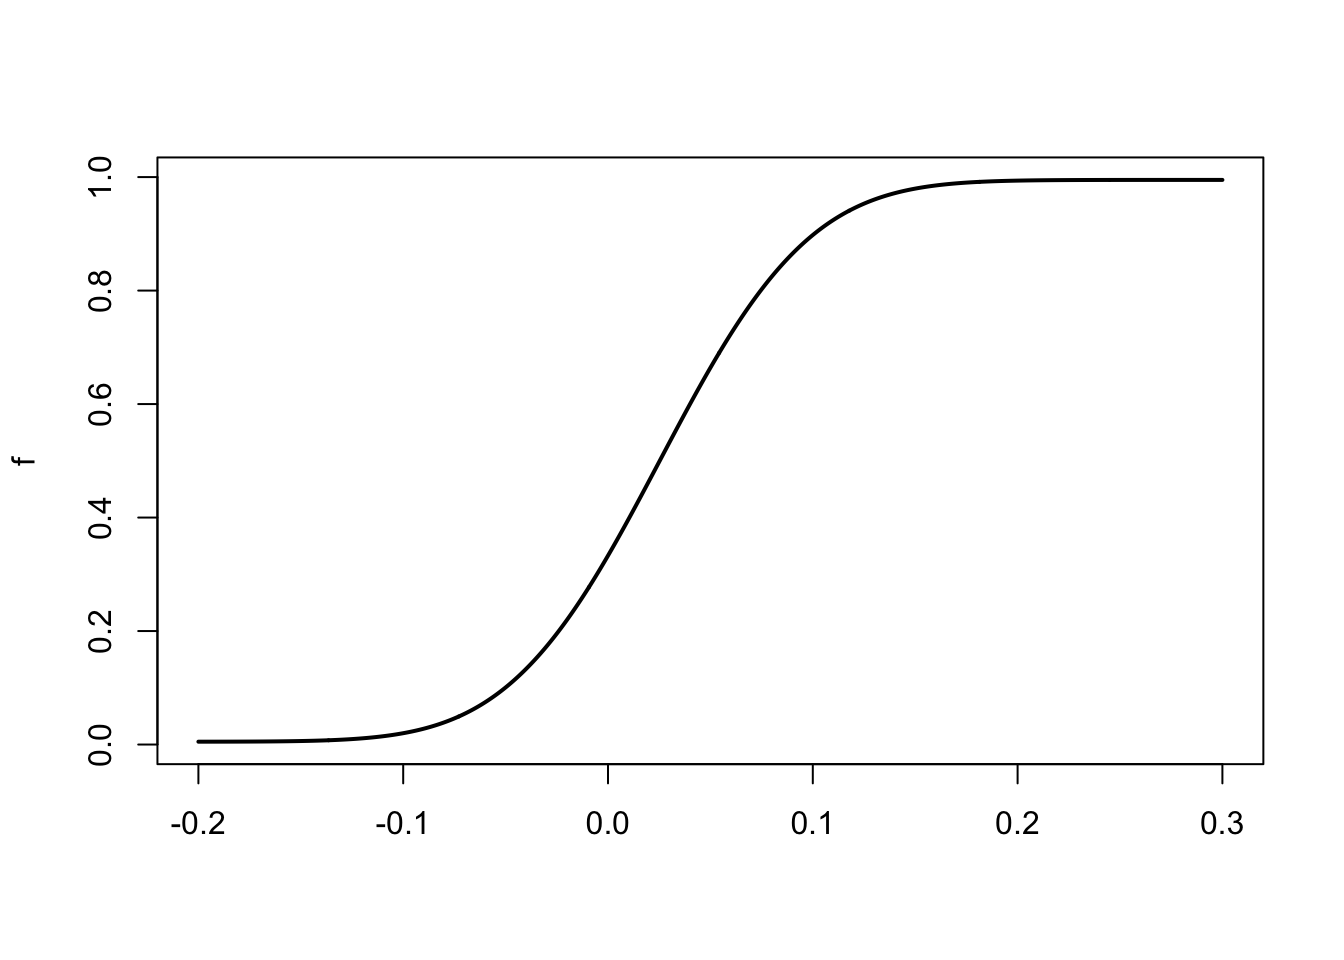
\includegraphics{TSM_files/figure-latex/truncatedRR-1} \caption{Conditional cumulated distribution function (c.d.f.) of $\frac{1}{H}(r_{t+1}+\dots+r_{t+H})$.}\label{fig:truncatedRR}
\end{figure}

\end{example}

\hypertarget{appendices}{%
\section{Appendices}\label{appendices}}

\begin{lemma}
\protect\hypertarget{lem:integralQuadratic}{}\label{lem:integralQuadratic}If \(\mu \in \mathbb{R}^L\) and \(Q\) is a \((L \times L)\) matrix symmetric positive definite, then:
\[
\int_{\mathbb{R}^{L}} \exp(-u'Q u + \mu'u)du =
\frac{\pi^{L/2}}{(det   Q)^{1/2}} exp \left(
\begin{array}{l}  \frac{1}{4} \mu'Q^{-1}\mu \end{array} \right).
\]
\end{lemma}

\begin{proof}
The integral is:
\begin{eqnarray*}
&& \int_{\mathbb{R}^{L}} exp \left[ \begin{array}{l} - (u -
\frac{1}{2}  Q^{-1} \mu)'  Q (u -
\frac{1}{2} Q^{-1} \mu)'
\end{array}
\right] exp\left(
\begin{array}{l}  \frac{1}{4} \mu'Q^{-1}\mu \end{array}
\right)du \\
&=&  \frac{\pi^{L/2}}{(det Q)^{1/2}} exp\left(
\begin{array}{l}  \frac{1}{4} \mu'Q^{-1}\mu \end{array}
\right)
\end{eqnarray*}
{[}using the formula for the unit mass of \(\mathcal{N}( 0.5Q^{-1}\mu,(2Q)^{-1})\){]}.
\end{proof}

\begin{lemma}
\protect\hypertarget{lem:Quadr}{}\label{lem:Quadr}If \(\varepsilon_{t+1} \sim \mathcal{N}(0,Id)\), we have
\[
\mathbb{E}_t \left(\exp[\lambda'\varepsilon_{t+1}+\varepsilon'_{t+1} V \varepsilon_{t+1}]\right) =  \frac{1}{[\det(I-2V)]^{1/2}} \exp\left[
\frac{1}{2} \lambda'(I-2V)^{-1}\lambda
\right].
\]
\end{lemma}

\begin{proof}
We have
\[
\mathbb{E}_t   \exp(\lambda'\varepsilon_{t+1}+\varepsilon'_{t+1}V\varepsilon_{t+1})
=  \frac{1}{(2\pi)^{n/2}}  \int_{\mathbb{R}^{n}} \exp\left[
\begin{array}{l}
-u'\left(
\begin{array}{l}
\frac{1}{2} I-V
\end{array}
\right)u+\lambda'u
\end{array}
\right]du
\]
From Lemma \ref{lem:integralQuadratic}, if \(u\in\mathbb{R}^n\), then
\[
\int_{\mathbb{R}^{n}} \exp(-u' Q u+\mu'u) du =
\frac{\pi^{n/2}}{(\det Q)^{1/2}} \exp\left(
\begin{array}{l}
\frac{1}{4} \mu'Q^{-1}\mu
\end{array}
\right).
\]
Therefore:
\[
\begin{array}{l}
\mathbb{E}_t   \exp(\lambda'\varepsilon_{t+1}+\varepsilon'_{t+1}V\varepsilon_{t+1}) \\
=  \frac{1}{2^{n/2}
\left[
\begin{array}{l}
\det \left(
\begin{array}{l}
\frac{1}{2} I-V
\end{array}
\right)
\end{array}
\right]^{1/2}
}
\exp\left[
\begin{array}{l}
\frac{1}{4}  \lambda'\left(
\begin{array}{l}
\frac{1}{2} I-V
\end{array}
\right)^{-1}\lambda
\end{array}
\right].
\end{array}
\]
\end{proof}

\begin{proposition}[Quadratic Gaussian process]
\protect\hypertarget{prp:QGVAR1}{}\label{prp:QGVAR1}Consider vector \(w_t = (x'_t,vec(x_t x_t')')'\), where \(x_t\) is a \(n\)-dimensional vector following a Gaussian VAR(1), i.e.
\[
x_{t+1}|\underline{w_t} \sim \mathcal{N}(\mu+\Phi x_t, \Sigma).
\]
If \(u = (v,V)\) where \(v \in \mathbb{R}^n\) and \(V\) a square symmetric matrix of size \(n\), we have:
\begin{eqnarray*}
\varphi_t(u) &=& \mathbb{E}_t\big\{\exp\big[(v',vec(V)')\times w_{t+1}\big]\big\} \\
& =& \exp \left\{a_1(v,V)'x_t +vec(a_2(v,V))' vec(x_t'x_t) + b(v,V) \right\},
\end{eqnarray*}
where:
\begin{eqnarray*}
a_2(u) & = & \Phi'V (I_n - 2\Sigma V)^{-1} \Phi \nonumber \\
a_1(u) & = & \Phi'\left[(I_n-2V\Sigma)^{-1}(v+2V\mu)\right] \nonumber \\
b(u) & = & u'(I_n - 2 \Sigma V)^{-1}\left(\mu + \frac{1}{2} \Sigma v\right) +\\
&& \mu'V(I_n - 2 \Sigma V)^{-1}\mu - \frac{1}{2}\log\big|I_n - 2\Sigma V\big|.\label{eq:laplaceZ}
\end{eqnarray*}
\end{proposition}

\begin{proof}
We have:
\begin{eqnarray*}
&&\mathbb{E}_t(\exp(v' x_{t+1} + vec(V)'vec(x_{t+1} x_{t+1}'))) \\
&=& \mathbb{E}_t[\exp(v' (\mu + \Phi x_t + \Sigma^{1/2}\varepsilon_{t+1}) + \\
&& vec(V)'vec((\mu + \Phi x_t + \Sigma^{1/2}\varepsilon_{t+1}) (\mu + \Phi x_t + \Sigma^{1/2}\varepsilon_{t+1})'))] \\
&=& \exp[v' (\mu + \Phi x_t) + vec(V)'vec\{(\mu + \Phi x_t)(\mu + \Phi x_t)'\}] \times \\
&& \mathbb{E}_t[\exp(v'\Sigma^{1/2}\varepsilon_{t+1} +2\underbrace{ vec(V)' vec\{(\mu + \Phi x_t)(\varepsilon_{t+1}'{\Sigma^{1/2}}')\}}_{=(\mu + \Phi x_t)'V\Sigma^{1/2}\varepsilon_{t+1}} +\\
&& \underbrace{vec(V)'vec\{(\Sigma^{1/2}\varepsilon_{t+1})(\Sigma^{1/2}\varepsilon_{t+1})'}_{=\varepsilon_{t+1}'{\Sigma^{1/2}}'V\Sigma^{1/2}\varepsilon_{t+1}}\}]
\end{eqnarray*}
Lemma \ref{lem:Quadr} can be used to compute the previous conditional expectation, with \(\lambda = {\Sigma^{1/2}}'(v + 2 V'(\mu + \Phi x_t))\). Some algebra then leads to the result.
\end{proof}

\begin{proposition}[]
\protect\hypertarget{prp:LTARG}{}\label{prp:LTARG}Consider the following auto-regressive gamma process:
\[
\frac{w_{t+1}}{\mu} \sim \gamma(\nu+z_t) \quad \mbox{where} \quad z_t \sim \mathcal{P} \left( \frac{\rho w_t}{\mu} \right),
\]
with \(\nu\), \(\mu\), \(\rho > 0\). (Alternatively \(z_t \sim {\mathcal{P}}(\beta w_t)\), with \(\rho = \beta \mu\).)

We have:
\(\varphi_t(u) = exp \left[ \begin{array}{l} \dfrac{\rho u}{1-u \mu} w_t - \nu \log(1-u \mu)\end{array} \right], \mbox{ for } u < \dfrac{1}{\mu}\).
\end{proposition}

\begin{proof}
Given \(\underline{w_t}\), we have \(z_t \sim {\mathcal P}\left( \begin{array}{l} \frac{\rho w_t} {\mu} \end{array}\right)\). We have:
\begin{eqnarray*}
\mathbb{E}[\exp(u w_{t+1})|\underline{w_t}] &=& \mathbb{E}\left\{\mathbb{E}\left[\exp \left(u \mu  \frac{w_{t+1}}{\mu}\right)|\underline{w_t}, \underline{z}_t\right]\underline{w_t}\right\}\\
&=& \mathbb{E}[(1-u\mu)^{-(\nu+z_t)}|\underline{w_t}] \\
&=& (1-u\mu)^{-\nu}\mathbb{E}\{\exp[-z_t   \log(1-u\mu)]|\underline{w_t}\} \\
&=& (1-u\mu)^{-\nu} \exp \left\{\frac{\rho w_t}{\mu}[\exp(-\log(1-u\mu)] -  \frac{\rho w_t}{\mu}\right\}\\
&=& \exp\left[ \begin{array}{l}  \frac{\rho u w_t}{1-u\mu} - \nu   \log(1-u\mu)  \end{array}\right],
\end{eqnarray*}
using the fact that the L.T. of \(\gamma(\nu)\) is \((1-u)^{-\nu}\)
and that the L.T. of \({\mathcal P}(\lambda)\) is \(\exp[\lambda(\exp(u)-1)]\).
\end{proof}

\begin{proposition}[Dynamics of a WAR process]
\protect\hypertarget{prp:WARAR}{}\label{prp:WARAR}If \(K\) is an integer, \(W_{t+1}\) can be obtained from:
\begin{eqnarray*}
\left\{
\begin{array}{ccl}
W_{t+1} & =&  \sum^K_{k=1} x_{k,t+1} x'_{k,t+1}\\
&&\\
x_{k,t+1} & =& M x_{k,t} + \varepsilon_{k,t+1},\quad k \in \{1,\dots,K\},
\end{array}
\right.
\end{eqnarray*}
where \(\varepsilon_{k,t+1} \sim i.i.d. \mathcal{N}(0, \Omega)\) (independent across \(k\)'s).
In particular, we have:
\[
\mathbb{E}(W_{t+1}|\underline{W_t}) = MW_tM'+K \Omega,
\]
i.e.~\(W_t\) follows a matrix weak AR(1) process.
\end{proposition}

\begin{proof}
For \(K=1\), \(W_{t+1}=x_{t+1} x'_{t+1}\), \(x_{t+1} = M x_t + \Omega^{1/2} u_{t+1}\) and \(u_{t+1} \sim i.i.d. \mathcal{N}(0,Id_L)\). We have:
\[
\mathbb{E}[\exp(Tr \Gamma W_{t+1})|\underline{w_t}] = \mathbb{E}\{\mathbb{E}[\exp(Tr \Gamma x_{t+1} x'_{t+1})|\underline{x}_t]|\underline{w_t}\}
\]
and:
\begin{eqnarray*}
&& \mathbb{E}[\exp(Tr \Gamma x_{t+1}x'_{t+1})|\underline{x}_t] = \mathbb{E}[\exp(x'_{t+1}\Gamma x_{t+1}|\underline{x}_t] \\
&=& \mathbb{E}[\exp(M x_t + \Omega^{1/2} u_{t+1})'\Gamma(M x_t + \Omega^{1/2} u_{t+1})/x_t] \\
&=& \exp(x'_tM'\Gamma M x_t)\mathbb{E}[\exp(2 x'_t M'\Gamma \Omega^{1/2}
u_{t+1}+u'_{t+1}\Omega^{1/2} \Gamma \Omega^{1/2} u_{t+1})/x_t] \\
&=&  \frac{exp(x'_tM'\Gamma M x_t)}{(2\pi)^{L/2}} \times \\
&& \int_{\mathbb{R}^L} \exp\left[2x'_tM'\Gamma
\Omega^{1/2}u_{t+1}-u'_{t+1}\left(
\frac{1}{2} Id_L-\Omega^{1/2} \Gamma \Omega^{1/2}\right)u_{t+1}\right]  du_{t+1}.
\end{eqnarray*}
Using Lemma \ref{lem:integralQuadratic} with \(\mu' = 2 x'_t M'\Gamma \Omega^{1/2}, Q = \frac{1}{2} Id_L-\Omega^{1/2}\Gamma\Omega^{1/2}\) \textbackslash{}
and after some algebra, the RHS becomes:
\[
\frac{exp[x'_tM'\Gamma(Id_L-2\Omega\Gamma)^{-1}M
x_t]}{det[Id_L-2\Omega^{1/2}\Gamma\Omega^{1/2}]} =  \frac{exp Tr[M'\Gamma(Id_L-2\Omega^{-1}]M
W_t]}{det[Id_L-2\Omega \Gamma]^{1/2}},
\]
which depends on \(x_t\) through \(W_t\), and gives the result for
\(K=1\); the result for any \(K\) integer follows.
\end{proof}

\begin{lemma}
\protect\hypertarget{lem:MHLT}{}\label{lem:MHLT}We have:
\[
\varphi_{t,h}(\gamma_1,\dots,\gamma_h) = \exp(A'_{t,h} w_t + B_{t,h}),
\]
where \(A_{t,h} = A^h_{t,h}\) and \(B_{t,h} = B^h_{t,h}\), the \(A^h_{t,i}, B^h_{t,i}\) \(i = 1,\dots,h\), being given recursively by:
\[
(i) \left\{
\begin{array}{ccl}
A^h_{t,i} &=& a_{t+h+1-i}(\gamma_{h+1-i} + A^h_{t,i-1}), \\
B^h_{t,i} &=& b_{t+h+1-i}(\gamma_{h+1-i} + A^h_{t,i-1}) + B^h_{t,i-1}, \\
A^h_{t,0} &=& 0, B^h_{t,0} = 0.
\end{array}
\right.
\]
\end{lemma}

\begin{proof}
For any \(j=1,\dots,h\) we have:
\[
\varphi_{t,h}(\gamma_1,\dots,\gamma_h) = \mathbb{E}_t[\exp(\gamma'_1 w_{t+1}+\dots\gamma'_j w_{t+j}+A^{h'}_{t,h-j}w_{t+j}+B^h_{t,h-j})]
\]
where:
\[
(ii) \left\{
\begin{array}{l}
A^h_{t,h-j+1} = a_{t+j}(\gamma_{j} + A^h_{t,h-j}), \\
B^h_{t,h-j+1} = b_{t+j}(\gamma_{j} + A^h_{t,h-j}) + B^h_{t,h-j}, \\
A^h_{t,0} = 0, B^h_{t,0} = 0.
\end{array}
\right.
\]
Since this is true for \(j=h\), and if this is true for \(j\), we get:
\[
\begin{array}{ll}
\varphi_{t,h}(\gamma_1,\dots,\gamma_h) & = \mathbb{E}_t [\exp(\gamma'_1 w_{t+1}+\dots+\gamma'_{j-1}w_{t+j-1}+a'_{t+j}(\gamma_j+A^h_{t,h-j})w_{t+j-1} \\
& + b_{t+j}(\gamma_j+A^h_{t,h-j})+B^h_{t,h-j}],
\end{array}
\]
and, therefore, this is true for \(j-1\), with \(A^h_{t,h-j+1}\) and \(B^h_{t,h-j+1}\) given by formulas (ii) above.

For \(j=1\) we get:
\begin{eqnarray*}
\varphi_{t,h}(\gamma_1,\dots,\gamma_h) &=& \mathbb{E}_t \exp(\gamma'_1 w_{t+1}+A^{h'}_{t,h-1}w_{t+1}+B^h_{t,h-1}) \\
&=& \exp(A'_{t,h} w_t+B_{t,h}),
\end{eqnarray*}

Finally note that if we put \(h-j+1 = i\), formulas (ii) become (i).
\end{proof}

\begin{proposition}[Reverse-order multi-horizon Laplace transform]
\protect\hypertarget{prp:reverseMLT}{}\label{prp:reverseMLT}If the functions \(a_{t}\) and \(b_{t}\) do not depend on \(t\), and if different sequences \((\gamma^h_1,\dots,\gamma^h_h), h=1,\dots,H\) (say) satisfy \(\gamma^h_{h+1-i} = u_i\), for
\(i=1,\dots,h\), and for any \(h \leq H\), that is if we want to compute (``reverse order'' case):
\[
\varphi_{t,h}(u_h,\dots,u_1)=\mathbb{E}_t[\exp(u'_{{\color{red}h}} w_{{\color{red}t+1}}+\dots+u'_{{\color{red}1}} w_{{\color{red}t+h}})],
\quad h=1,\dots,H,
\]
then we can compute the \(\varphi_{t,h}(u_h,\dots,u_1)\) for any \(t\) and any \(h \leq H\), with only one recursion, i.e.~\(\varphi_{t,h}(u_h,\dots,u_1)=\exp(A'_hw_t+B_h)\) with:
\begin{equation}
\left\{
\begin{array}{ccl}
A_{h} &=& a(u_{h} + A_{h-1}), \\
B_{h} &=& b(u_{h} + A_{h-1}) + B_{h-1}, \\
A_{0} &=& 0,\quad  B_{0} = 0.
\end{array}
\right.\label{eq:auxLemmareverseMLT}
\end{equation}
\end{proposition}

\begin{proof}
According to Lemma \ref{lem:MHLT}, we have, in this case:
\[
\left\{
\begin{array}{ccl}
A^h_{i} &=& a(u_{i} + A^h_{i-1}), \\
B^h_{i} &=& b(u_{i} + A^h_{i-1}) + B^h_{i-1}, \\
A^h_{0} &=& 0, \quad B^h_{0} = 0.
\end{array}
\right.
\]
The previous sequences do not dependent on \(h\) and are given by Eq. \eqref{eq:auxLemmareverseMLT}.
\end{proof}

\begin{proposition}[Conditional means and variances of an affine process]
\protect\hypertarget{prp:condvarAffine}{}\label{prp:condvarAffine}Consider an affine process \(w_t\). Using the notation of Proposition \ref{prp:affineVAR}, we have:
\begin{eqnarray}
\mathbb{E}_t(w_{t+h}) &=& (I - \Phi)^{-1}(I - \Phi^h)\mu + \Phi^h w_t \label{eq:condmeanAppendix}\\
\mathbb{V}ar_t(w_{t+h}) &=& \Sigma(\mathbb{E}_t(w_{t+h-1}))+\Phi \Sigma(\mathbb{E}_t(w_{t+h-2}))\Phi' + \nonumber \\
&& \dots + \Phi^{h-1} \Sigma(w_{t}){\Phi^{h-1}}'. \label{eq:condvarAppendix}
\end{eqnarray}
Eq. \eqref{eq:condvarAppendix} notably shows that \(\mathbb{V}ar_t(w_{t+h})\) is an affine function of \(w_t\). Indeed \(\Sigma(.)\) is an affine function, and the conditional expectations \(\mathbb{E}_t(w_{t+h})\) are affine in \(w_t\), as shown by Eq. \eqref{eq:condmeanAppendix}.

The unconditional mean and variance of \(w_t\) are given by:
\begin{equation}
\left\{
\begin{array}{ccl}
\mathbb{E}(w_t) &=& (I - \Phi)^{-1}\mu\\
vec[\mathbb{V}ar(w_t)] &=& (I_{n^2} - \Phi \otimes \Phi)^{-1} vec\left(\Sigma[(I - \Phi)^{-1}\mu]\right).
\end{array}
\right.\label{eq:uncondmeanvarAppendix}
\end{equation}
\end{proposition}

\begin{proof}
Eq. \eqref{eq:condmeanAppendix} is easily deduced from Eq. \eqref{eq:VARw}, using that \(\mathbb{E}_t(\varepsilon_{t+k})=0\) for \(k>0\).

As regards Eq. \eqref{eq:condvarAppendix}:
\begin{eqnarray*}
\mathbb{V}ar_t(w_{t+h}) &=& \mathbb{V}ar_t\left(\Sigma(w_{t+h-1})^{\frac{1}{2}}\varepsilon_{t+h}+\dots + \Phi^{h-1} \Sigma(w_{t})^{\frac{1}{2}}\varepsilon_{t+1} \right).
\end{eqnarray*}
The conditional expectation at \(t\) of all the terms of the sum is equal to zero since, for \(i \ge 1\):
\[
\mathbb{E}_t\left[\Sigma(w_{t+i-1})^{\frac{1}{2}}\varepsilon_{t+i}\right] = \mathbb{E}_t[\underbrace{\mathbb{E}_{t+i-1}\{\Sigma(w_{t+i-1})^{\frac{1}{2}}\varepsilon_{t+i}\}}_{=\Sigma(w_{t+i-1})^{\frac{1}{2}}\mathbb{E}_{t+i-1}\{\varepsilon_{t+i}\}=0}\}],
\]
and \(\forall i <j\),
\[
\mathbb{C}ov_t\left[\Sigma(w_{t+i-1})^{\frac{1}{2}}\varepsilon_{t+i},\Sigma(w_{t+j-1})^{\frac{1}{2}}\varepsilon_{t+j}\right] = \mathbb{E}_t\left[\Sigma(w_{t+i-1})^{\frac{1}{2}}\varepsilon_{t+i}\varepsilon_{t+j}'\Sigma'(w_{t+j-1})^{\frac{1}{2}}\right],
\]
which can be seen to be equal to zero by conditioning on the information available on date \(t+j-1\).

Using the same conditioning, we obtain that:
\begin{eqnarray*}
\mathbb{V}ar_t\left[\Phi^{h-j}\Sigma(w_{t+j-1})^{\frac{1}{2}}\varepsilon_{t+j}\right] &=& \mathbb{E}_t\left[\Phi^{h-j}\Sigma(w_{t+j-1})^{\frac{1}{2}}\varepsilon_{t+j}\varepsilon_{t+j}'\Sigma'(w_{t+j-1})^{\frac{1}{2}}{\Phi^{h-j}}'\right] \\
&=&  \mathbb{E}_t\left[\Phi^{h-j}\Sigma(w_{t+j-1})^{\frac{1}{2}} \mathbb{E}_{t+j-1}(\varepsilon_{t+j}\varepsilon_{t+j}')\Sigma'(w_{t+j-1})^{\frac{1}{2}}{\Phi^{h-j}}'\right] \\
&=&  \Phi^{h-j}\mathbb{E}_t[\Sigma(w_{t+j-1})]{\Phi^{h-j}}' \\
&=&  \Phi^{h-j}\Sigma(\mathbb{E}_t[w_{t+j-1}]){\Phi^{h-j}}',
\end{eqnarray*}
where the last equality results from the fact that he fact that \(\Sigma(.)\) is affine (see Eq. \eqref{eq:SigmaWt}).
\end{proof}

\begin{proposition}[Affine property of the GARCH-type process]
\protect\hypertarget{prp:GARCH}{}\label{prp:GARCH}The process \(w_t = (w_{1,t}, w_{2,t})\) defined by:
\[
\left\{
\begin{array}{ccl}
w_{1, t+1} &=& \mu + \varphi w_{1,t} + \sigma_{t+1} \varepsilon_{t+1}    \mid \varphi \mid < 1 \\
\sigma^2_{t+1} &=& \omega + \alpha \varepsilon^2_t + \beta \sigma^2_t      0 < \beta < 1, \alpha > 0, \omega > 0    \\
w_{2,t} &=& \sigma^2_{t+1}, \quad \varepsilon_t \sim   i.i.d.   \mathcal{N}(0,1)
\end{array}
\right.
\]
is affine.
\end{proposition}

\begin{proof}
Note that \(w_{2,t}\) is function of \(\underline{w_{1,t}}\)
\begin{eqnarray*}
&& \mathbb{E}[\exp(u_1 w_{1, t+1} + u_2 w_{2, t+1})|\underline{w_{1,t}}] \\
&= & \exp(u_1 \mu + u_1 \varphi w_{1,t} + u_2 \omega + u_2 \beta w_{2,t})  \mathbb{E}[\exp(u_1 \sigma_{t+1} \varepsilon_{t+1} + u_2 \alpha \varepsilon^2_{t+1})|\underline{w_{1,t}}]
\end{eqnarray*}
and, using Lemma \ref{lem:Quadr}:
\begin{eqnarray*}
&&\mathbb{E}[\exp(u_1 w_{1, t+1} + u_2 w_{2, t+1})|\underline{w_{1,t}}] \\
&= & \exp(u_1 \mu + u_1 \varphi w_{1,t} + u_2 \omega + u_2 \beta w_{2t})  \exp \left[ -   \frac{1}{2}   \log(1-2 u_2 \alpha) +
\frac{u^2_1 w_{2,t}}{2(1-2 u_2 \alpha)} \right]\\
&= & \exp \left[ u_1 \mu + u_2 \omega -  \frac{1}{2}   \log(1-2u_2\alpha)+  u_1 \varphi w_{1,t} + \left(u_2 \beta +  \frac{u^2_1}{2(1-2u_2\alpha)}\right)
w_{2,t}\right],
\end{eqnarray*}
which is exponential affine in \((w_{1,t}, w_{2,t})\).
\end{proof}

\begin{proposition}[Computation of truncated conditional moments]
\protect\hypertarget{prp:Fourier}{}\label{prp:Fourier}If \(\varphi(z)=\mathbb{E}[exp(z'w)]\), we have:
\begin{equation}
\mathbb{E}[\exp(u'w)\textbf{1}_{(v'w<\gamma})] = \frac{\varphi(u)}{2} -  \frac{1}{\pi} \int^\infty_o
\frac{{\mathcal I}m[\varphi(u+ivx)\exp(-i\gamma x)]}{x}dx.\label{eq:Truncated}
\end{equation}
\end{proposition}

\begin{proof}
We want to compute \(\tilde{\varphi}_t(u;v,\gamma) = \mathbb{E}_t[\exp(u'w)\textbf{1}_{(v'w<\gamma})]\). Let us first note that, for given \(u\) and \(v\), \(\tilde{\varphi}_t(u;v,\gamma)\) is a positive increasing bounded function of \(\gamma\) and therefore can be seen as the c.d.f. of a positive finite measure on \(\mathbb{R}\), the Fourier transform of which is:
\[
\int_{\mathbb{R}} \exp(i\gamma x)d\tilde{\varphi}(u;v,\gamma) = \mathbb{E} \int_{\mathbb{R}} \exp(i\gamma x)d\tilde{\varphi}_w(u;v,\gamma),
\]
where, for given \(w, \tilde{\varphi}_w(u;v,\gamma)\) is the c.d.f. of the mass point \(\exp(u'w)\) at \(v'w\). We then get:
\begin{eqnarray*}
\int_{\mathbb{R}} \exp(i\gamma x) d\tilde{\varphi}(u;v,\gamma) &=& \mathbb{E}[\exp(ixv'w)exp(u'w)] \\
& =& \mathbb{E}[\exp(u+ivx)'w] \\
& =& \varphi(u+ivx).
\end{eqnarray*}
Let us now compute \(A(x_0,\lambda)\) for any real number \(\lambda\), with:
\begin{eqnarray*}
&&A(x_0,\lambda) \\
&=&  \frac{1}{2\pi} \int^{x_0}_{-x_0}
\frac{\exp(i\lambda x)\varphi(u-ivx)-\exp(-i\lambda)\varphi(u+ivx)}{ix}dx \\
&=&  \frac{1}{2\pi} \int^{x_0}_{-x_0}\left[ \begin{array}{l}  \int_{\mathbb{R}}
\frac{\exp[-ix(\gamma-\lambda)]-\exp[ix(\gamma-\lambda)]}{ix}d\tilde{\varphi}(u;v,\gamma)
\end{array} \right]dx \\
&=&  \frac{1}{2\pi}  \int_{\mathbb{R}}
\left[ \begin{array}{l}   \int^{x_0}_{-x_0}   \frac{\exp[-ix(\gamma-\lambda)]
-\exp[ix(\gamma-\lambda)]}{ix}dx \end{array} \right]d\tilde{\varphi}(u;v,\gamma).
\end{eqnarray*}
Now :
\begin{eqnarray*}
\frac{1}{2\pi} \int^{x_o}_{-x_o}
\frac{\exp[-ix(\gamma-\lambda)]
-\exp[ix(\gamma-\lambda)]}{ix}dx \\ =  \frac{-sign(\gamma-\lambda)}{\pi}
\int^{x_o}_{-x_o} \frac{sin(x\mid\gamma-\lambda\mid)}{x}dx
\end{eqnarray*}
which tends to \(-sign(\gamma-\lambda)\) when \(x_0\rightarrow\infty\) (where \(sign(\omega)=1\) if \(\omega>0\), \(sign(\omega)=0\) if \(\omega=0\), \(sign(\omega)=-1\) if \(\omega<0\)).
Therefore:
\[
A(\infty,\lambda) = -  \int_{\mathbb{R}} sign(\gamma-\lambda)d\tilde{\varphi}(u;v,\gamma) = -\mathbb{E}  \int_{\mathbb{R}} sign(\gamma-\lambda)d\tilde{\varphi}_w(u;\theta,\gamma),
\]
where \(\tilde{\varphi}_w(u;v,\gamma)\) is the c.d.f. of the mass point \(\exp(u'w)\) at \(v'w\) and
\[
\int_{\mathbb{R}} \mbox{sign}(\gamma-\lambda)d\tilde{\varphi}_w(u;v,\gamma)=
\left\{
\begin{array}{ccc}
\exp(u'w) & \mbox{if} & \lambda < v'w \\
0 & \mbox{if}& \lambda = v'w \\
-\exp(u'w) & \mbox{if} & \lambda > v'w.
\end{array}
\right.
\]
Therefore, we have:
\begin{eqnarray*}
A(\infty,\lambda) & =& - \mathbb{E}[\exp(u'w)(1-\textbf{1}_{(v'w<\lambda)})-\exp(u'w)\textbf{1}_{(v'w<\lambda)}] \\
& =& - \varphi(u) + 2\tilde{\varphi}(u;v,\lambda)
\end{eqnarray*}
and, further,:
\[
\tilde{\varphi}(u;,v,\gamma) =  \frac{\varphi(u)}{2} +  \frac{1}{2} A(\infty,\gamma),
\]
where
\begin{eqnarray*}
\frac{1}{2} A(\infty,\gamma) & =&  \frac{1}{4\pi} \int^{\infty}_{-\infty}  \frac{\exp(i\gamma x)\varphi(u-ivx)-\exp(-i\gamma x)\varphi(u+ivx)}{ix} dx \\
& =&  \frac{1}{2\pi} \int^{\infty}_{o}  \frac{\exp(i\gamma x)\varphi(u-ivx)-\exp(-i\gamma x)\varphi(u+ivx)}{ix} dx \\
& =& -  \frac{1}{\pi} \int^{\infty}_{o}  \frac{{\mathcal I}m[\exp(-i\gamma x)\varphi(u+ivx)]}{x}dx,
\end{eqnarray*}
which leads to Eq. \eqref{eq:Truncated}.
\end{proof}

\hypertarget{pricing-and-risk-neutral-dynamics}{%
\chapter{Pricing and risk-neutral dynamics}\label{pricing-and-risk-neutral-dynamics}}

\hypertarget{PricingEquilibrium}{%
\section{Consumption-based Capital Asset Pricing Model (CCAPM) and stochastic discount factor (SDF)}\label{PricingEquilibrium}}

Consider an economy featuring a single good, whose date-\(t\) price is \(q_t\). There is a representative agent with an external income \(R_t\) at \(t\), and a portfolio of assets, with an allocation vector \(\alpha_{t-1}\) (decided at \(t-1\)). The vector of date-\(t\) prices is \(p_t\). At any date \(t+j\), \(j=0,1,...\), the agent will face the budget constraint:
\[
q_{t+j}C_{t+j}+\alpha'_{t+j}p_{t+j} = R_{t+j} +
\alpha'_{t+j-1}p_{t+j},
\]
where \(C_{t+j}\)is her consumption on date \(t+j\). The representative agent maximizes her expected utility time-separable preferences \(\mathbb{E}_t \sum^\infty_{j=0} \delta^j U(C_{t+j})\) subject to the budget constraints at \(t+j\), \(j= 0,1,\dots\), where \(U\) is the utility function and \(\delta\)is time discount factor or subjective discount factor. Note that the latter is different from SDF.

Replacing \(C_{t+j}\) with \([R_{t+j}-(\alpha'_{t+j}-\alpha'_{t+j-1})p_{t+j}]/q_{t+j}\), the objective function becomes:
\[
\mathbb{E}_t  \sum^\infty_{j=0} \delta^j U
[R_{t+j}/q_{t+j}-(\alpha'_{t+j}-\alpha'_{t+j-1})p_{t+j}/q_{t+j}].
\]
The vector of allocation \(\alpha_t\) appears in the first two terms:
\[
U[R_t/q_t-(\alpha'_t-\alpha'_{t-1})p_t/q_t] + \delta \mathbb{E}_t
U[R_{t+1}/q_{t+1}-(\alpha'_{t+1}-\alpha'_t)p_{t+1}/q_{t+1}].
\]
As a result, the first order condition associated with vector \(\alpha_t\) reads
\[
\frac{p_t}{q_t}  \frac{d U(C_t)}{dC} = \delta \mathbb{E}_t \left[
\begin{array}{l}
\frac{p_{t+1}}{q_{t+1}}  \frac{dU(C_{t+1})}{dC}
\end{array}
\right],
\]
or
\begin{equation}
p_t = \mathbb{E}_t(p_{t+1} \mathcal{M}_{t,t+1}),\label{eq:SDF100}
\end{equation}
where \(\mathcal{M}_{t,t+1}\) is a strictly positive scalar called \textbf{stochastic discount factor (SDF)} between dates \(t\) and \(t+1\). We have:
\[
\mathcal{M}_{t,t+1} \equiv \delta  \frac{q_t}{q_{t+1}} 
\frac{  \frac{dU(C_{t+1})}{dC}} {
\frac{dU(C_t)}{dC}}.
\]

\begin{example}[Power utility function]
\protect\hypertarget{exm:CCAPM}{}\label{exm:CCAPM}A standard case is the one of the power utility \(U(C) = \frac{C^{1-\gamma}-1}{1-\gamma}\), where \(\gamma>0\) is the coefficient of relative risk aversion.

We have \(U'(C) = C^{-\gamma} > 0\) and \(U''(C) = - \gamma C^{-\gamma-1} < 0\). As a result, the stochastic discount factor is
\begin{eqnarray}
&& \mathcal{M}_{t,t+1} \nonumber \\
&=&  \frac{q_t}{q_{t+1}} \delta \left(
\frac{C_{t+1}}{C_t} \right)^{-\gamma} \nonumber\\
&=& \exp(\log
\delta + \log q_t + \gamma \log  C_t - \log  q_{t+1} - \gamma
\log  C_{t+1}).\label{eq:powerutilSDF}
\end{eqnarray}
The vector of prices \(p_t\) satisfies:
\[
p_t = \delta q_t C^\gamma_t \mathbb{E}_t \left(
\begin{array}{l}
\frac{C^{-\gamma}_{t+1}}{q_{t+1}} p_{t+1}
\end{array}
\right),
\]
or (Euler equation):
\[
\mathbb{E}_t\left[
\begin{array}{l}
\delta\left(
\begin{array}{l}
\frac{C_{t+1}}{C_t}
\end{array}
\right)^{-\gamma}  \frac{q_t}{q_{t+1}}
\frac{p_{t+1}}{p_t} - 1
\end{array}
\right] = 0.
\]
\end{example}

According to Eq. \eqref{eq:SDF100}, for any asset \(j\):
\begin{equation}
p_{j,t} = \mathbb{E}_t(\mathcal{M}_{t,t+1} p_{j,t+1}).\label{eq:Mbasicpricing}
\end{equation}
Using that \(p_{j,t+1} = \mathbb{E}_t(\mathcal{M}_{t+1,t+2} p_{j,t+2})\), we get:
\begin{eqnarray*}
p_{j,t} &=& \mathbb{E}_t[\mathbb{E}_{t+1}(p_{j,t+2}\mathcal{M}_{t+1,t+2})\mathcal{M}_{t,t+1}] \\
&=& \mathbb{E}_t(\mathcal{M}_{t,t+1} \mathcal{M}_{t+1,t+2}p_{j,t+2}).
\end{eqnarray*}
This can be generalized as follows:
\[
p_{j,t} = \mathbb{E}_t[\mathcal{M}_{t,t+1} \dots \mathcal{M}_{t+h-1,t+h}p_{j,t+h}], \; \forall h.
\]

\hypertarget{recursive-utilities}{%
\section{Recursive utilities}\label{recursive-utilities}}

XXXX

\hypertarget{PricingAAO}{%
\section{SDF: Absence of Arbitrage Approach}\label{PricingAAO}}

Consider a period of interest \({\mathcal T} = \{0,1,2,...,T^*\}\). As in Chapter \ref{ChapterAffine}, vector \(w_t\) constitutes the new information in the economy at \(t\). The historical, or physical, dynamics of \(w_t\), \(f(\underline{w_t})\), is defined by \(f(w_{t+1}|\underline{w_t})\). The physical probability is denoted by \(\mathbb{P}\). \(L_{2t}, t \in {\mathcal T}\), is the (Hilbert) space of square integrate functions \(g(\underline{w_t})\), and we have \(L_{2t} \subset L_{2s}, t< s\).

\hypertarget{existence-and-unicity-of-the-sdf}{%
\subsection{Existence and unicity of the SDF}\label{existence-and-unicity-of-the-sdf}}

\begin{hypothesis}[Price existence and uniqueness]
\protect\hypertarget{hyp:Apricing1}{}\label{hyp:Apricing1}For any \(\underline{w_t}\), there exists a unique \(p_t[g(\underline{w_s})]\),
function of \(\underline{w_t}\), price at \(t\) of a payoff
\(g(\underline{w_s})\) delivered at \(s, \forall t \le s\).
\end{hypothesis}

\begin{hypothesis}[Linearity and continuity]
\protect\hypertarget{hyp:Apricing2}{}\label{hyp:Apricing2}

For all \(t < s\), \(\underline{w_t}\), \(g_1\), \(g_2\), we have

\begin{itemize}
\tightlist
\item
  \(p_t[\lambda_1 g_1(\underline{w_s}) + \lambda_2g_2(\underline{w_s})] = \lambda_1p_t[g_1(\underline{w_s})]+\lambda_2 p_t[g_2(\underline{w_s})]\),
\item
  If \(g_n(\underline{w_s}) \overset{L_{2s}}{\underset{n\rightarrow\infty}{\longrightarrow}} 0\), then \(p_t[g_n(\underline{w_s})] \underset{n\rightarrow\infty}{\longrightarrow} 0\).
\end{itemize}

\end{hypothesis}

\begin{hypothesis}[Absence of Arbitrage Opportunity (AAO)]
\protect\hypertarget{hyp:Apricing3}{}\label{hyp:Apricing3}

At any \(t\), it is impossible to constitute a portfolio of future payoffs, possibly modified at subsequent dates, such that:

\begin{itemize}
\tightlist
\item
  the price of the portfolio at \(t\) is zero,
\item
  payoffs at subsequent dates are \(\ge 0\),
\item
  there is at least one subsequent date \(s\) such that the net payoff at \(s\) is strictly positive with a non zero conditional probability at \(t\).
\end{itemize}

\end{hypothesis}

\begin{theorem}[Riesz representation theorem]
\protect\hypertarget{thm:Riesz}{}\label{thm:Riesz}Under Assumptions \ref{hyp:Apricing1} and \ref{hyp:Apricing2}, for all \(\underline{w_t}\), and \(s > t\), there exists \(\mathcal{M}_{t,s}(\underline{w_s}) \in L_{2s}\), unique such that, \(\forall g(\underline{w_s}) \in L_{2s}\),
\[
p_t[g(\underline{w_s})] = \mathbb{E}[\mathcal{M}_{t,s}(\underline{w_s})g(\underline{w_s})|\underline{w_t}].
\]
In particular the price at \(t\) of a zero coupon bond maturing at \(s\) is \(\mathbb{E}(\mathcal{M}_{t,s}|\underline{w_t})\).
\end{theorem}

\begin{proposition}[Positivity of M]
\protect\hypertarget{prp:PositivityM}{}\label{prp:PositivityM}If Assumption \ref{hyp:Apricing3} is satisfied, then for all \(t\) and \(s\), \(\mathbb{P}(\mathcal{M}_{t,s}>0|\underline{w_t})=1\).
\end{proposition}

\begin{proof}
\(\Leftarrow\) is obvious. If \(\Rightarrow\) was not true, the payoff
\(\textbf{1}_{\{\mathcal{M}_{t,s} \le 0\}}\), at \(s\), would be such that:
\(\mathbb{P}[\textbf{1}_{\{\mathcal{M}_{t,s} \le 0\}}=1|\underline{w_t}] > 0\) and \(p_t[\textbf{1}_{\{\mathcal{M}_{t,s} \le 0\}}] = \mathbb{E}_t[\mathcal{M}_{t,s}\textbf{1}_{\{\mathcal{M}_{t,s} \le 0\}}] \le 0\).
\end{proof}

\begin{proposition}[Time consistency]
\protect\hypertarget{prp:timeconsist}{}\label{prp:timeconsist}For all \(t < r < s\), we have \(\mathcal{M}_{t,s} = \mathcal{M}_{t,r} \mathcal{M}_{r,s}\), which implies:
* \(\mathcal{M}_{t,s} = \mathcal{M}_{t,t+1} \mathcal{M}_{t+1,t+2}\dots\mathcal{M}_{s-1,s}\)
* \(\mathcal{M}_{0,t} = \Pi^{t-1}_{j=0} \mathcal{M}_{j,j+1}\) (\(\mathcal{M}_{0,t}\) is called \textbf{pricing kernel}).
\end{proposition}

\begin{proof}
Using Lemma \ref{lem:sdf} we have:
\begin{eqnarray*}
p_t(g_s) &=& \mathbb{E}(\mathcal{M}_{t,s}g_s|\underline{w_t}) = \mathbb{E}(\mathcal{M}_{t,r} p_r(g_s)|\underline{w_t}) \\
&=& \mathbb{E}[\mathcal{M}_{t,r}\mathbb{E}(\mathcal{M}_{r,s} g_s|\underline{w_r})|\underline{w_t}] = \mathbb{E}(\mathcal{M}_{t,r} \mathcal{M}_{r,s} g_s|\underline{w_t}), \forall g, \forall \underline{w}_{t}
\end{eqnarray*}
and, therefore, \(\mathcal{M}_{t,s} = \mathcal{M}_{t,r}\mathcal{M}_{r,s}\).
\end{proof}

\begin{lemma}
\protect\hypertarget{lem:sdf}{}\label{lem:sdf}For any payoff \(g_s\) at \(s, p_t(g_s) = p_t[p_r(g_s)]\).
\end{lemma}

\begin{proof}
If this was not true, we could construct a sequence of portfolios with a strictly positive payoff at \(s\) with zero payoff at any other future date and with price zero at \(t\), contradicting Assumption \ref{hyp:Apricing3}. Indeed, assuming, for instance, \(p_t(g_s) > p_t[p_r(g_s)]\), the payoff at \(s\) is defined by the following strategy: (i) at \(t\): buy \(p_r(g_s)\), (short) sell \(g_s\), buy
\(\frac{p_t(g_s)-p_t[p_r(g_s)]}{\mathbb{E}(\mathcal{M}_{t,s}|\underline{w_t})}\) zero-coupon bonds maturing at \(s\), at global price zero, (ii) at \(r\): buy \(g_s\) and sell \(p_r(g_s)\), generating a zero net payoff, (iii) at \(s\), the net payoff is: \(g_s-g_s+\frac{p_t(g_s)-p_t[p_r(g_s)]}{\mathbb{E}(\mathcal{M}_{t,s}|\underline{w_t})} > 0\).
\end{proof}

Consider an asset whose payoff, on date \(s\), is \(g(\underline{w_s})\). We have, \(\forall t < s\):
\begin{equation}
\boxed{p_t[g(\underline{w_s})] = \mathbb{E}_t[\mathcal{M}_{t,t+1}...\mathcal{M}_{s-1,s}g(\underline{w_s})].}\label{eq:basic}
\end{equation}
In particular, since \(L_{2,t+1}\) contains 1, the price at \(t\) of a zero-coupon with residual maturity one is given by:
\[
B(t,1) := \mathbb{E}_t [\mathcal{M}_{t,t+1}].
\]
Denoting by \(r_t\) the continously-compounded interest rate, defined through \(B(t,1)=\exp(-r_{t})\), we get
\[
r_{t}=-\log \mathbb{E}_t [\mathcal{M}_{t,t+1}].
\]

\begin{definition}[Bank account]
\protect\hypertarget{def:bankaccount}{}\label{def:bankaccount}The bank account process \(R_t\) is defined by \(R_{t} \equiv \exp(r_0+...+r_{t-1}) = \frac{1}{\mathbb{E}_0[ \mathcal{M}_{0,1}]\times ... \times \mathbb{E}_{t-1} [\mathcal{M}_{t-1,t}]}\).

\(R_t\) is the price of an investment initiated on date 0, when it was worth one dollar, and invested on each date at the risk-free rate (for one period).
\end{definition}

For any price process \(p_t\), we have \(p_t = \mathbb{E}_t(\mathcal{M}_{t,s} p_s)\) (with \(s>t\)), or \(\mathcal{M}_{0,t} p_t = \mathbb{E}_t(\mathcal{M}_{0,s}p_s)\). That is, \(\mathcal{M}_{0,t} p_t\) is a martingale. In particular \(\mathcal{M}_{0,t} R_t\) is a martingale.

\hypertarget{PricingAffine}{%
\subsection{Exponential Affine SDF}\label{PricingAffine}}

A specific (tractable) case is that of exponential affine SDF. Assume that
\[
\mathcal{M}_{t,t+1}(\underline{w_{t+1}}) = \exp[\alpha_t(\underline{w_t})'w_{t+1}+\beta_t(\underline{w_t})]
\]
where \(\alpha_t\) defines the \emph{factor loadings} or \emph{sensitivity} vector. Using \(\mathbb{E}_t[\mathcal{M}_{t,t+1}]=\exp(-r_{t})=\exp[\psi_t(\alpha_t)+\beta_t]\), we get:
\begin{equation}
\mathcal{M}_{t,t+1} = \exp[-r_{t}+\alpha'_tw_{t+1}-\psi_t(\alpha_t)].\label{eq:keySDF}
\end{equation}

\begin{example}[CCAPM/Power utility case]
In the CCAPM-power-utility case (see Example \ref{exm:CCAPM}), we have (Eq. \eqref{eq:powerutilSDF}):
\[
\mathcal{M}_{t,t+1} = \exp(\log \delta + \log q_t + \gamma \log   C_t - \log   q_{t+1} - \gamma  \log   C_{t+1}),
\]
where \(q_t\) is the price of the consumption good, \(C_t\) is the quantity consumed at \(t\) and \(\delta\) is the intertemporal discount rate.

Hence, in that case, \(\mathcal{M}_{t,t+1}\) is exponential affine in \(w_{t+1} = (\log q_{t+1}, \log C_{t+1})'\) (and its first lag).
\end{example}

\hypertarget{PricingRN}{%
\section{The risk-neutral (R.N.) dynamics}\label{PricingRN}}

The historical Dynamics is characterized by \(f(\underline{w_{T^*}})\), or by the
sequence of conditional p.d.f. \(f_{t+1}(w_{t+1}|\underline{w_t})\), or
\(f_{t+1}(w_{t+1})\), with respect to (w.r.t.) some measure \(\mu\).

We define the conditional risk-neutral p.d.f. w.r.t. the conditional historical probability. For that, we employ the Radon-Nikodym derivative \(d^{\mathbb{Q}}_{t+1}(w_{t+1}|\underline{w_t})\):
\[
d^{\mathbb{Q}}_{t+1}(w_{t+1}|\underline{w_t}) =
\frac{\mathcal{M}_{t,t+1}(\underline{w_{t+1}})}{\mathbb{E}[\mathcal{M}_{t,t+1}(\underline{w_{t+1}})|\underline{w_t}]},
\]
or
\[
d^{\mathbb{Q}}_{t+1}(w_{t+1})=
\frac{\mathcal{M}_{t,t+1}}{\mathbb{E}_t(\mathcal{M}_{t,t+1})}=\exp(r_{t}) \mathcal{M}_{t,t+1}.
\]
The risk neutral conditional p.d.f. is:
\begin{eqnarray}
f^{\mathbb{Q}}_{t+1}(w_{t+1}) &=& f_{t+1}(w_{t+1})d^{\mathbb{Q}}_{t+1}(w_{t+1}) \nonumber \\
&=&f_{t+1} (w_{t+1}) \mathcal{M}_{t,t+1} (\underline{w_{t+1}}) \exp [r_{t} (\underline{w_t})].\label{eq:fQfP}
\end{eqnarray}
Of course, the conditional historical p.d.f. with respect to the conditional risk-neutral (R.N.) p.d.f. is:
\[
d_{t+1}(w_{t+1}) =
\frac{1}{d^{\mathbb{Q}}_{t+1}(w_{t+1})} \quad \mbox{or}\quad d_{t+1}(w_{t+1}) =
\frac{\exp(-r_{t})}{\mathcal{M}_{t,t+1}}.
\]

The p.d.f. of \(\mathbb{Q}\) w.r.t. the historical dynamics \(\mathbb{P}\) is:
\[
\xi_{T^*} =  \frac{d\mathbb{Q}}{d\mathbb{P}} =
\Pi^{T^{*}-1}_{t=0} d^{\mathbb{Q}}_{t+1}(w_{t+1}) =
\Pi^{T^{*}-1}_{t=0} \exp(r_{t}) \mathcal{M}_{t,t+1}.
\]
Note that the p.d.f. of the R.N. distribution of \(\underline{w_t}\), w.r.t. the corresponding historical distribution is:
\[
\xi_t= \Pi^{t-1}_{\tau=1}
d^{\mathbb{Q}}_{\tau+1}(w_{\tau+1})=\mathbb{E}_t\left( \begin{array}{l}
\frac{d\mathbb{Q}}{d\mathbb{P}}
\end{array} \right) = \mathbb{E}_t\xi_{T^*}
\]
(and \(\xi_t\) therefore is a \(\mathbb{P}\)-martingale) since:
\[
\mathbb{E}_t \left( \frac{d\mathbb{Q}}{d\mathbb{P}}\right) = \Pi^{t-1}_{\tau = 1} d^{\mathbb{Q}}_{\tau + 1} (w_{\tau+1}) \mathbb{E}_t \left( d^{\mathbb{Q}}_{t+1} (w_{t+1}) \ldots d^{\mathbb{Q}}_{T^*} (w_{T^*})\right).
\]
* Equivalent form of the pricing formula (that is Eq. \eqref{eq:basic}):

Price at \(t\) of a payoff \(g(\underline{w_s})\) at time \(s>t\):
\begin{eqnarray}
p_t[g(\underline{w_s})] &=& \mathbb{E}_t[\mathcal{M}_{t,t+1}...\mathcal{M}_{s-1,s}g(\underline{w_s})] \\
&=& \mathbb{E}^{\mathbb{Q}}_t[exp(-r_{t}-...-r_{s-1})g(\underline{w_s})]\quad \mbox{(key
formula).}\nonumber
\end{eqnarray}
* Or, with simpler notations:
\begin{eqnarray*}
p_t &=& \mathbb{E}^{\mathbb{Q}}_t[exp(-r_{t}-...-r_{s-1})p_s] \\
&=& \mathbb{E}^{\mathbb{Q}}_t\left(\frac{R_t}{R_s} p_s\right) \quad (R_t:\mbox{bank account})
\end{eqnarray*}
\(\Rightarrow\) \(\dfrac{p_t}{R_t} = \mathbb{E}^{\mathbb{Q}}_t\left( \dfrac{p_s}{R_s}\right)\), that is, \(\dfrac{p_t}{R_t}\) is a
\(\mathbb{Q}\)-martingale.
* In particular:
\[
p_t = \exp(-r_{t})\mathbb{E}^{\mathbb{Q}}_t(p_{t+1})
\]
or, using the arithmetic return of any payoff
\[
\rho_{A,t+1}= \frac{p_{t+1}-p_t}{p_t}
\]
and the arithmetic return of the riskless asset \(r_{A,t+1}=exp(r_{t})-1\), we get (\textbf{key result}):
\[
\mathbb{E}^{\mathbb{Q}}_t(\rho_{A,t+1})=r_{A,t}.
\]
* Moreover the excess arithmetic return process \(\rho_{A,t+1}-r_{A,t}\) is a \(\mathbb{Q}\)-martingale difference and, therefore, \(\mathbb{Q}\)-serially uncorrelated.
* Case of an exponential affine SDF:
\[
\begin{array}{ll}
d^{\mathbb{Q}}_{t+1}(w_{t+1}) & =
\frac{\mathcal{M}_{t,t+1}}{\mathbb{E}_t(\mathcal{M}_{t,t+1})} =
\frac{\exp(\alpha'_t
w_{t+1}+\beta_t)}{\exp[\psi_t(\alpha_t)+\beta_t]} =
\frac{\exp(\alpha'_t w_{t+1})}{\varphi_t(\alpha_t)} \\
& = \exp[\alpha'_t w_{t+1}-\psi_t(\alpha_t)]
\end{array}
\]
\(\Rightarrow\) \(d^{\mathbb{Q}}_{t+1}(w_{t+1})\) is also exponential affine.
* We have:
\[
f^{\mathbb{Q}}_{t+1} (w_{t+1}) = \frac{f_{t+1} (w_{t+1}) \exp (\alpha'_t w_{t+1})}{\varphi_t (\alpha_t)}.
\]

\(f^{\mathbb{Q}}_{t+1}\) Esscher transform of \(f_{t+1}\), corresponding to \(\alpha_t\).

\begin{itemize}
\tightlist
\item
  Laplace transform of the conditional R.N. probability:
\end{itemize}

\(\varphi^{\mathbb{Q}}_t(u|\underline{w_t})\), also denoted by \(\varphi^{\mathbb{Q}}_t(u)\):
\begin{eqnarray*}
\varphi^{\mathbb{Q}}_t(u) &=& \mathbb{E}^{\mathbb{Q}}_t \exp(u' w_{t+1}) \\
&=& \mathbb{E}_t \exp[(u+\alpha_t)'w_{t+1}-\psi_t(\alpha_t)] \\
&=& \exp[\psi_t(u+\alpha_t)-\psi_t(\alpha_t)] =
\frac{\varphi_t(u+\alpha_t)}{\varphi_t(\alpha_t)}
\end{eqnarray*}

\(\Rightarrow\) (\textbf{key result})
\begin{equation}
\psi^{\mathbb{Q}}_t(u) = \psi_t(u+\alpha_t)-\psi_t(\alpha_t).\label{eq:transfoPQ}
\end{equation}
* We check that, if \(\alpha_t=0\), \(\psi^{\mathbb{Q}}_t=\psi_t\) (since \(\psi_t(0)=0)\).
* Back to the historical conditional probability:
\[
d_{t+1}(w_{t+1}) =
\frac{1}{d^{\mathbb{Q}}_{t+1}(w_{t+1})} = \exp[-\alpha'_t
w_{t+1}+\psi_t(\alpha_t)],
\]
* Putting \(u=-\alpha_t\) in the expression of
\(\psi^{\mathbb{Q}}_t(u)\) we get
\[
\psi^{\mathbb{Q}}_t(-\alpha_t)=-\psi_t(\alpha_t),
\]
and, replacing \(u\) by \(u-\alpha_t\), we get (\textbf{key result}):
\[
\psi_t(u) = \psi^{\mathbb{Q}}_t(u-\alpha_t)-\psi^{\mathbb{Q}}_t(-\alpha_t)
\]
Also:
\begin{equation*}
\left\{
\begin{array}{ccl}
d_{t+1}(w_{t+1}) &=& \exp[-\alpha'_t(w_{t+1})-\psi^{\mathbb{Q}}_t(-\alpha_t)] \\
d^{\mathbb{Q}}_{t+1}(w_{t+1}) &=& \exp[\alpha'_t(w_{t+1})+\psi^{\mathbb{Q}}_t(-\alpha_t)].
\end{array}
\right.
\end{equation*}

\hypertarget{PricingTypology}{%
\section{Typology of Econometric Asset Pricing Models}\label{PricingTypology}}

\begin{definition}[Econometric Asset Pricing Model (EAPM)]
\protect\hypertarget{def:typo}{}\label{def:typo}An Econometric Asset Pricing Model (EAPM) is defined by the following functions:

\emph{\(r_{t}(\underline{w_t})\),
} \(f(w_{t+1}|\underline{w_t}))\) {[}or \(\psi_t(u)\){]},
* \(\mathcal{M}_{t,t+1}(\underline{w_{t+1}})\),
* \(f^{\mathbb{Q}}(w_{t+1}|\underline{w_t})\) {[}or \(\psi^{\mathbb{Q}}_t(u)\){]}.
\end{definition}

\begin{itemize}
\item
  The previous functions have to to be specified and parameterized.
\item
  They are linked by:
  \[
  f^{\mathbb{Q}}(w_{t+1}|\underline{w_t}) = f(w_{t+1}|\underline{w_t}) \mathcal{M}_{t,t+1}(\underline{w_{t+1}}) \exp[r_{t}(\underline{w_t}))].
  \]
\item
  We are going to present three ways of specifying an EAPM:
\end{itemize}

\begin{enumerate}
\def\labelenumi{\arabic{enumi}.}
\tightlist
\item
  the Direct Modelling,
\item
  the R.N. Constrained Direct Modelling (or Mixed Modelling),
\item
  the Back Modelling.
\end{enumerate}

\begin{itemize}
\tightlist
\item
  If \(\mathcal{M}_{t,t+1}\) is exponential affine:
  \[
  \mathcal{M}_{t,t+1} (\underline{w_{t+1}}) = \exp \{ -r_{t} (\underline{w_t}) + \alpha'_t (\underline{w_t}) )
  w_{t+1} - \psi_t [\alpha_t (w_t)]\}.
  \]
\item
  Once \(r_{t} (\underline{w_t})\) is specified we have to specify \(\psi_t, \alpha_t, \psi^{\mathbb{Q}}_t\) linked by
  \[
  \psi^{\mathbb{Q}}_t (u) = \psi_t (u+\alpha_t) - \psi_t (\alpha_t).
  \]
\item
  In all approaches, we have to specify the status of the short rate \(r_{t}\) (developed in next slide).
\end{itemize}

\textbf{Remark}: The status of the short rate

The short rate \(r_{t}\) is a function of \(\underline{w_t}\), this function may be known or unknown by the econometrician:

\begin{enumerate}
\def\labelenumi{\roman{enumi}.}
\tightlist
\item
  It is known in two cases:
\end{enumerate}

\begin{enumerate}
\def\labelenumi{\alph{enumi}.}
\tightlist
\item
  \(r_{t}\) is exogenous \(\Rightarrow\) \(r_{t}(\underline{w_t})\) does not depend on \(\underline{w_t}\),
\item
  \(r_{t}\) is an endogenous factor \(\Rightarrow\) \(r_{t}\) is a component of \(w_t\).
\end{enumerate}

\begin{enumerate}
\def\labelenumi{\roman{enumi}.}
\setcounter{enumi}{1}
\tightlist
\item
  If the function \(r_{t} (\underline{w_t})\) is unknown, it has to be specified
  parametrically:
  \begin{equation*}
  \left\{ r_{t} (\underline{w_t}, \tilde{\theta}), \tilde{\theta}\in \tilde{\Theta} \right\},
  \end{equation*}
  where \(r_{t} (.,.)\) is a known function.
\end{enumerate}

\hypertarget{the-direct-modelling-based-on-threes-steps}{%
\subsection{The Direct Modelling (based on threes steps)}\label{the-direct-modelling-based-on-threes-steps}}

\begin{itemize}
\tightlist
\item
  \textbf{Step 1}: Specification of the historical dynamics
\end{itemize}

We choose a parametric family for the conditional historical Log-Laplace transform \(\psi_t (u | \underline{w_t})\):
\begin{equation*}
\left\{ \psi_t (u  |  \underline{w_t} ; \theta_1), \theta_1 \in \Theta_1 \right\} .
\end{equation*}
* \{\bf Step 2: Specification of the SDF\}
\begin{equation*}
\begin{array}{lll} \mathcal{M}_{t,t+1} &=& \exp \left[ -
r_{t} (\underline{w_t}) + \alpha'_t (\underline{w_t}) w_{t+1} -
\psi_t (\alpha_t | \underline{w_t}) \right];
\end{array}
\end{equation*}

Once \(r_{t}\) has been specified (\(r_{t}(\underline{w_t}, \tilde{\theta})\)), \(\alpha_t(\underline{w_t})\) remains to be specified. We assume
that \(\alpha_t (\underline{w_t})\) belongs to a parametric family:
\begin{equation*}
\left\{ \alpha_t (\underline{w_t} ; \theta_2),
\theta_2 \in \Theta_2 \right\}
\end{equation*}
\begin{eqnarray*}
\Rightarrow \mathcal{M}_{t,t+1}(\underline{w_{t+1}}, \theta) &=& \exp \left\{ - r_{t}
(\underline{w_t}, \tilde{\theta}) + \alpha'_t (\underline{w_t},\theta_2) w_{t+1} \right.\\
&& \left. - \psi_{t} \left[ \alpha_t (\underline{w_t},
\theta_2) | \underline{w_t} ; \theta_1 \right] \right\}
\end{eqnarray*}
\noindent where \(\theta = (\tilde{\theta}', \theta'_1, \theta'_2)' \in \tilde{\Theta}\times \Theta_1 \times \Theta_2 = \Theta\);

\(\tilde{\Theta}\) may be reduced to one point (Case i of Remark \textbf{ST}).

\begin{itemize}
\tightlist
\item
  \textbf{Step 3}: Internal consistency conditions (ICC)
\end{itemize}

For any payoff \(g(\underline{w_s})\) delivered at \(s>t\), with price \(p(\underline{w_t})\) at \(t\) which is a known function of
\(\underline{w_t}\), we must have:
\begin{equation*}\label{ICCgen}
p(\underline{w_t}) = \mathbb{E} \left\{\mathcal{M}_{t,t+1} (\theta)
... \mathcal{M}_{s-1,s} (\theta) g(\underline{w_s})  |  \underline{w_t},
\theta_1 \right\}    \forall \; \underline{w_t}, \theta .
\end{equation*}

These ICC pricing conditions may imply strong constraints on \(\theta\), for instance:

\begin{itemize}
\tightlist
\item
  When components of \(w_t\) are returns of some assets:
  \[
  \mbox{If }w_{1,t} = \log \dfrac{p_{1,t}}{p_{1,t-1}}, \mbox{ then }\mathbb{E}_t \mathcal{M}_{t,t+1} \exp (e'_1 w_{t+1}) = 1.
  \]
  or interest rates with various maturities:
  \begin{eqnarray*}
  &&\mbox{If }w_{1,t} = -\frac{1}{h}\log B(t,h), \\
  && \mbox{ then } e'_1 w_{t} = - \frac{1}{h} \log \mathbb{E}_t (\mathcal{M}_{t,t+1}\times \dots \times \mathcal{M}_{t+h-1,t+h}).
  \end{eqnarray*}
\item
  The previous three steps imply the specification of the R.N. dynamics:
  \begin{equation*}
  \psi^{\mathbb{Q}} (u | \underline{w_t}, \theta_1, \theta_2) =
  \psi_t \left[ u + \alpha_t (\underline{w_t}, \theta_2) |
  \underline{w_t}, \theta_1 \right] - \psi_t \left[ \alpha_t
  (\underline{w_t}, \theta_2) | \underline{w_t}, \theta_1
  \right].
  \end{equation*}
\end{itemize}

\hypertarget{the-r.n.-constrained-direct-modelling-or-mixed-modelling}{%
\subsection{The R.N. constrained direct modelling (or mixed modelling)}\label{the-r.n.-constrained-direct-modelling-or-mixed-modelling}}

\textbf{Step 1}: Specification of \(\mathbb{P}\)-dynamics

We select a family \(\{ \psi_t (u | \underline{w_t},\theta_1), \theta_1 \in \Theta_1 \}\):

{[}to explain, for instance, some stylized fact about \(w_t\){]}.

\textbf{Step 2}: Specification of \(\mathbb{Q}\)-dynamics

We select a family \(\{\psi^{\mathbb{Q}}_t (u | \underline{w_t}, \theta^*),\theta^* \in \Theta^* \}\) and possibly \(\{r_{t}(\underline{w_t},\tilde{\theta}),\tilde{\theta}\in\tilde{\Theta}\}\)

{[}to have explicit or quasi explicit pricing formula{]}.

\textbf{Step 3}: Internal Consistency Conditions (ICC)

Once the parameterization \((\tilde{\theta}, \theta_1, \theta^*) \in \tilde{\Theta} \times \Theta^*_1\) is
defined, ICCs may be imposed:
\begin{eqnarray*}
&&\mbox{If }w_{1,t} = \log \frac{p_{1,t}}{p_{1,t-1}}, \mbox{ then } \exp(-r_t)\mathbb{E}^{\mathbb{Q}}_t \exp (e_{1}' w_{t+1}) = 1\\
&&\mbox{If }w_{1,t} = B(t,h), \mbox{ then } e_{1}' w_{t} = \mathbb{E}_t^{\mathbb{Q}} \exp(-r_t - \dots - r_{t+h-1}).
\end{eqnarray*}

\begin{itemize}
\tightlist
\item
  The SDF is a by-product and, if we want an exponential affine SDF, for any pair \((\psi^{\mathbb{Q}}_t, \psi_t)\) belonging to these families, there must exist a unique function \(\alpha_t (\underline{w_t})\) denoted by \(\alpha_t (w_t ; \theta_1, \theta^*)\), and satisfying:
  \begin{equation*}
  \psi^{\mathbb{Q}}_t (u | \underline{w_t}) = \psi_t \left[ u +
  \alpha_t (w_t) | \underline{w_t} \right] - \psi_t \left[
  \alpha_t (\underline{w_t}) | \underline{w_t} \right].
  \end{equation*}
\end{itemize}

\hypertarget{the-back-modelling-based-on-three-steps}{%
\subsection{The Back Modelling (based on three steps)}\label{the-back-modelling-based-on-three-steps}}

\textbf{Step 1}: Specification of the R.N. dynamics\} {[}and possibly of \(r_{t}(\underline{w_t})\){]}: \(\psi^{\mathbb{Q}}_t (u | \underline{w_t}; \theta^*_1)\).

\textbf{Step 2}: Internal consistency conditions (ICC) \} --if relevant-- are taken into account:
\begin{equation*}
\begin{array}{lll}
&& p(\underline{w_t}) = \mathbb{E}^{\mathbb{Q}}_t \left[ \exp (-r_{t} (\underline{w_t}, \tilde{\theta})
- \ldots - r_{s-1} (\underline{w_s}, \tilde{\theta}))g (\underline{w_s}) | \underline{w_t} , \theta^*_1
\right] ,\\
&& \forall    \underline{w_t} , \tilde{\theta} , \theta^*_1.
\end{array}
\end{equation*}
\textbf{Step 3}: Choice of the specification of \(\alpha_t(\underline{w_t})\)\} (without any constraint), providing the family \(\{ \alpha_t (\underline{w_t}, \theta^*_2),\theta^*_2\in \Theta^*_2 \}\).
* The historical dynamics is a by-product:
\begin{equation*}
\psi_t(u | \underline{w_t} ; \theta^*_1, \theta^*_2) = \psi^{\mathbb{Q}}_t
\left[ u - \alpha_t (\underline{w_t}, \theta^*_2) |
\underline{w_t} ; \theta^*_1 \right] - \psi^{\mathbb{Q}}_t \left[
- \alpha_t (\underline{w_t}, \theta^{
*}_2) | \underline{w_t}, \theta^*_1 \right].
\end{equation*}

\hypertarget{the-term-structure-of-risk-free-yields}{%
\section{THE TERM STRUCTURE OF RISK-FREE YIELDS}\label{the-term-structure-of-risk-free-yields}}

\begin{Shaded}
\begin{Highlighting}[]
\FunctionTok{library}\NormalTok{(ecb)}
\NormalTok{rates }\OtherTok{\textless{}{-}} \FunctionTok{get\_data}\NormalTok{(}
  \CommentTok{\#"YC.B.U2.EUR.4F.G\_N\_A.SV\_C\_YM.SR\_10Y",}
  \StringTok{"FM.M.U2.EUR.4F.BB.R\_U2\_10Y.YLDA"}\NormalTok{,}
  \AttributeTok{filter=}\FunctionTok{list}\NormalTok{(}\AttributeTok{startPeriod=}\StringTok{"1991{-}12"}\NormalTok{))}
\FunctionTok{plot}\NormalTok{(}\FunctionTok{as.Date}\NormalTok{(}\FunctionTok{paste}\NormalTok{(rates}\SpecialCharTok{$}\NormalTok{obstime,}\StringTok{"{-}15"}\NormalTok{,}\AttributeTok{sep=}\StringTok{""}\NormalTok{)),rates}\SpecialCharTok{$}\NormalTok{obsvalue,}\AttributeTok{type=}\StringTok{"l"}\NormalTok{)}
\NormalTok{spf }\OtherTok{\textless{}{-}} \FunctionTok{get\_data}\NormalTok{(}
  \StringTok{"SPF.Q.U2.HICP.POINT.LT.Q.AVG"}\NormalTok{,}
  \AttributeTok{filter=}\FunctionTok{list}\NormalTok{(}\AttributeTok{startPeriod=}\StringTok{"1991{-}12"}\NormalTok{))}
\NormalTok{spf}\SpecialCharTok{$}\NormalTok{obstime }\OtherTok{\textless{}{-}} \FunctionTok{gsub}\NormalTok{(}\StringTok{"Q1"}\NormalTok{, }\StringTok{"02{-}15"}\NormalTok{, spf}\SpecialCharTok{$}\NormalTok{obstime)}
\NormalTok{spf}\SpecialCharTok{$}\NormalTok{obstime }\OtherTok{\textless{}{-}} \FunctionTok{gsub}\NormalTok{(}\StringTok{"Q2"}\NormalTok{, }\StringTok{"05{-}15"}\NormalTok{, spf}\SpecialCharTok{$}\NormalTok{obstime)}
\NormalTok{spf}\SpecialCharTok{$}\NormalTok{obstime }\OtherTok{\textless{}{-}} \FunctionTok{gsub}\NormalTok{(}\StringTok{"Q3"}\NormalTok{, }\StringTok{"08{-}15"}\NormalTok{, spf}\SpecialCharTok{$}\NormalTok{obstime)}
\NormalTok{spf}\SpecialCharTok{$}\NormalTok{obstime }\OtherTok{\textless{}{-}} \FunctionTok{gsub}\NormalTok{(}\StringTok{"Q4"}\NormalTok{, }\StringTok{"11{-}15"}\NormalTok{, spf}\SpecialCharTok{$}\NormalTok{obstime)}
\FunctionTok{lines}\NormalTok{(}\FunctionTok{as.Date}\NormalTok{(}\FunctionTok{paste}\NormalTok{(spf}\SpecialCharTok{$}\NormalTok{obstime,}\StringTok{"{-}15"}\NormalTok{,}\AttributeTok{sep=}\StringTok{""}\NormalTok{)),spf}\SpecialCharTok{$}\NormalTok{obsvalue,}\AttributeTok{lty=}\DecValTok{3}\NormalTok{)}
\end{Highlighting}
\end{Shaded}

\begin{figure}
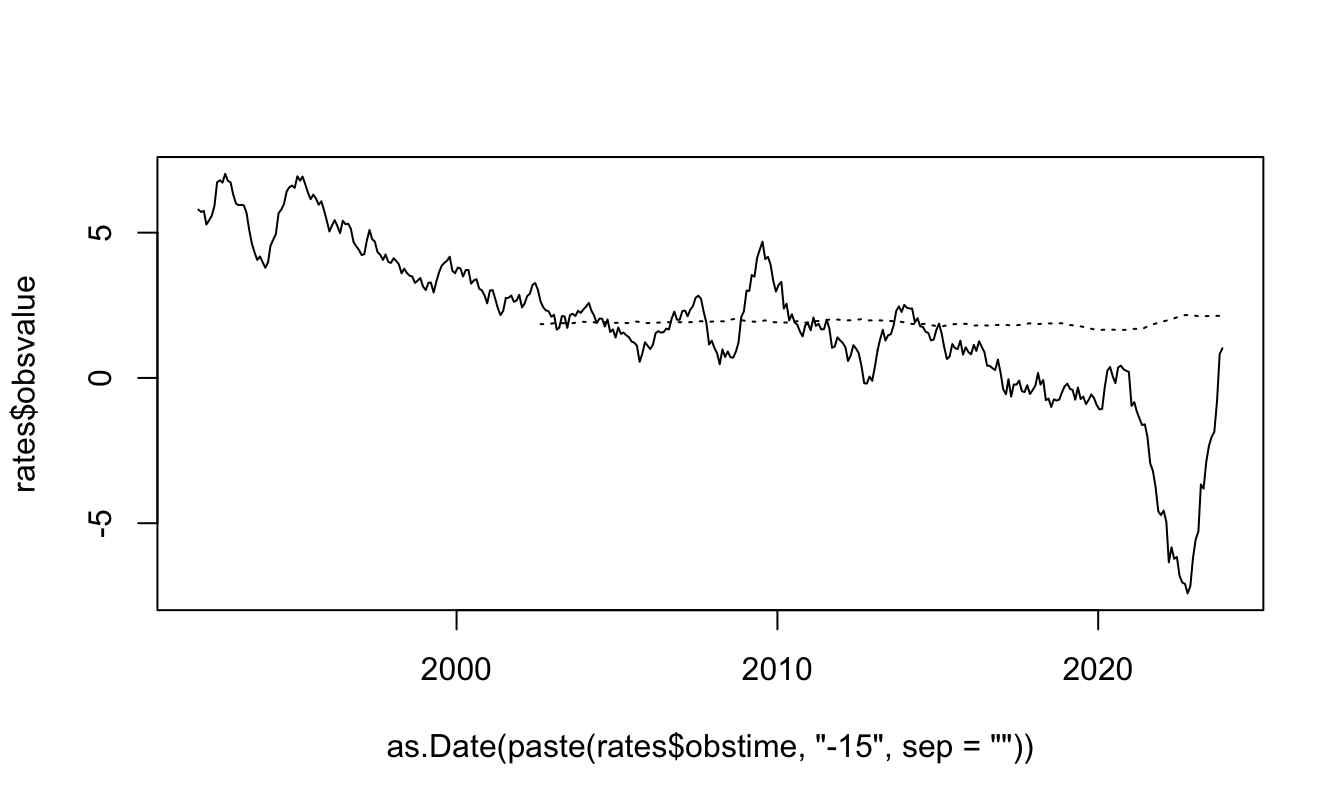
\includegraphics[width=0.95\linewidth]{TSM_files/figure-latex/extractECB-1} \caption{Simulation of a quadratic processes $x_t$.}\label{fig:extractECB}
\end{figure}

\hypertarget{RFIntroduction}{%
\subsection{Introduction}\label{RFIntroduction}}

\begin{itemize}
\item
  \textbf{Risk-free} = with no default (and/or liquidity) risks.
\item
  An important share of the term-structure literature pertains to the modelling of risk-free yields.
\item
  Some models involve macro factors (in \(w_t\)). Some do not (\emph{yield-only} models).
\item
  Basic formula (see Eq. \eqref{eq:stdbond} in Example \ref{exm:nominalBth}):
  \begin{eqnarray}
  B(t,h) &=& \exp(-r_{t}) \mathbb{E}^{\mathbb{Q}}_t \exp(-r_{t+1}-\dots-r_{t+h-1})\\
  R(t,h) &=& - \frac{1}{h} \log B(t,h). \label{eq:stdbondRFchapter}
  \end{eqnarray}
\item
  Models used to forecast yields, or to compute \textbf{term premiums} = components of yields that would not exist if investors were not risk-averse.
\item
  If this was the case (\textbf{Expectation Hypothesis, EH}), then \(\mathcal{M}_{t,t+1} = \exp(- r_t) \Rightarrow\) ``\(\mathbb{P} \equiv \mathbb{Q}\)'\,' and \(B(t,h)\) would become:
  \begin{equation}
  \exp(-r_{t}) \mathbb{E}_t \exp(-r_{t+1}-\dots-r_{t+h-1}).\label{eq:stdbondRFchapterP}
  \end{equation}
  implying that the maturity-\(h\) yield-to-maturity would be:
  \[
  R^{EH}(t,h) = -\frac{1}{h}\log \left( \mathbb{E}_t \exp(-r_t-\dots-r_{t+h-1})\right) \approx \frac{1}{h}\mathbb{E}_t(r_t + \dots + r_{t+h-1}).
  \]
\end{itemize}

\(\Rightarrow\) Term premium given by:
\begin{eqnarray}
TP_{t,h} &=& \underbrace{- \frac{1}{h} \log  \mathbb{E}^{\mathbb{Q}}_t \exp(-r_{t+1}-\dots-r_{t+h-1})}_{=R(t,h)} - \nonumber \\
&& \underbrace{- \frac{1}{h}  \log  \mathbb{E}_t \exp(-r_{t+1}-\dots-r_{t+h-1}).}_{=R^{EH}(t,h)}\label{eq:TP}
\end{eqnarray}
* Interpretation of \(TP_{t,h}\)?
* Under EH, investors are willing to buy a maturity-\(h\) bond as long as its expected return is -- up to Jensen's inequality -- equal to the average of future short-term rates (Hence the definition of \(R^{EH}(t,h)\)).
* \(TP_{t,h}>0\) means that, due to risk aversion, investors are willing to buy the maturity-\(h\) bond only if its return is, on average, higher than expected future short-term rates.

\(\Rightarrow\) Reflects the fact that investors consider that long-term bonds tend to lose value in \textbf{bad states of the world}.

\hypertarget{RP}{%
\subsection{Risk premiums}\label{RP}}

\begin{itemize}
\tightlist
\item
  Recall Eq. (\eqref{eq:Mbasicpricing}), satisfied by any asset \(j\):
  \[
  p_{jt} = \mathbb{E}_t(\mathcal{M}_{t,t+1} p_{j,t+1}).
  \]
\item
  Can be rewritten:
  \[
  p_{jt} =  \mathbb{C}ov_t(\mathcal{M}_{t,t+1}, p_{j,t+1}) + \mathbb{E}_t(\mathcal{M}_{t,t+1})\mathbb{E}_t( p_{j,t+1})
  \]
  or
  \begin{equation}
  p_{jt} = \underbrace{\exp(-r_t)\mathbb{E}_t( p_{j,t+1})}_{=p^{EH}_{jt}} + \underbrace{\mathbb{C}ov_t(\mathcal{M}_{t,t+1}, p_{j,t+1})}_{\mbox{Risk premium}}.\label{eq:CovRP}
  \end{equation}
\item
  If investors were not risk-averse, then we would have \(p_{jt} = p^{EH}_{jt}\).
\item
  S.D.F. is high (resp. low) in \emph{bad (resp. good) states of the world} (states of high marginal utility in the equilibrium approach).
\end{itemize}

\(\Rightarrow\) \(p_{jt}< p^{EH}_{jt}\) if asset \(j\) tends to pay less in bad states of the world (i.e.~if \(\mathbb{C}ov_t(\mathcal{M}_{t,t+1}, p_{j,t+1})<0\)).

\hypertarget{swap-rates}{%
\subsection{Swap rates}\label{swap-rates}}

\begin{itemize}
\tightlist
\item
  Bonds issued by top-rated (Aaa/AAA) countries are often considered to be risk-free.
\item
  Because of call-margins mechanisms, swap rates are also used as risk-free benchmarks \href{https://www.aeaweb.org/articles?id=10.1257/jep.29.2.191}{Duffie and Stein (2015)}.
\item
  \textbf{Interest Rate Swap (IRS)}: Contract at \(t\) between a \emph{receiver} (of fixed rate) and a \emph{payer} (of fixed rate); the receiver pays a floating rate to the payer.
\item
  The dates of payment are \(t+ \tau\), \(t + 2\tau\), \ldots, \(t + n\tau\), where \(\tau\) is a period expressed in years (typically 1/2 or 1/4) and \(n\) is the number of payments.
\item
  \(h = n \tau\) is the maturity, or \emph{tenor} of the swap contract.
\item
  The payoffs of the fixed leg are \(\tau S\), where \(S\) is the annualized payment (or \emph{swap rate}). On date \(t+j\tau\), the payoff of the floating leg is \(\tau L(t+(j-1)\tau,\tau)\), where \(L\), the annualized linear rate is given by:
  \[
  L(t+(j-1)\tau,\tau) = \frac{1 - B(t+(j-1)\tau,\tau)}{\tau B(t+(j-1)\tau,\tau)}.
  \]
\item
  Price at \(t\) of the fixed leg:
  \[
  \sum_{j=1}^n \tau S B(t,j\tau).
  \]
\item
  Price at \(t\) of the floating leg: The payoff at date \(t+j\tau\), that is \(\frac{1 - B(t+(j-1)\tau,\tau)}{B(t+(j-1)\tau,\tau)}\) is know on date \(t+(j-1)\tau\), so its price at date \(t+(j-1)\tau\) is \(1 - B(t+(j-1)\tau,\tau)\), and its price at \(t\) therefore is \(B(t,(j-1)\tau) - B(t,j\tau)\). Summing over \(j=1,\dots,n\), the date-\(t\) price of the floating leg is \(1 - B(t,n\tau)\) (independent of the payment dates).
\item
  Since the price of the contract is zero at date \(t\), we have:
  \[
  \sum_{j=1}^n \tau S B(t,j\tau) = 1 - B(t,n\tau) \Rightarrow S = \frac{1 - B(t,n\tau)}{ \tau \sum_{j=1}^n  B(t,j\tau)},
  \]
  or
  \[
  S(t,h) = \frac{1 - B(t,h)}{\tau \sum_{j=1}^{h/\tau}  B(t,j\tau)}.
  \]
\item
  Note: In the context of an affine model, all the terms appearing in the previous formula are available in closed-form (see Example \ref{exm:nominalBth}).
\end{itemize}

\hypertarget{RiskFreeAffine}{%
\section{The Affine Case}\label{RiskFreeAffine}}

\begin{itemize}
\item
  What do we get when \(w_t\) is affine (under \(\mathbb{P}\) and \(\mathbb{Q}\))?
\item
  If the nominal short-term rate \(r_t = \omega_0 + \omega'_1 w_t\), then:
  \begin{eqnarray*}
  B(t,h) &=& \mathbb{E}^{\mathbb{Q}}_t \exp (-r_{t}-\dots-r_{t+h-1})\\
  &=& \exp(-h\omega_0 - \omega'_1 w_t) \color{blue}{\mathbb{E}^{\mathbb{Q}}_t \exp (- \omega'_1 w_{t+1}-\dots- \omega'_1 w_{t+h-1})}.
  \end{eqnarray*}
  The (blue) expectation is easily computed using the recursive equations of XXX (see Example \ref{exm:nominalBth}), leading to:
  \begin{equation}
  R(t,h)= -  \frac{1}{h}   \log   B(t,h) = A_h'w_t + B_h.\label{eq:RthAB}
  \end{equation}
\item
  It is easily seen that we can also get:
  \begin{equation}
  R^{EH}(t,h) = {A^{EH}_h}'w_t + B^{EH}_h.\label{eq:RthABEH}
  \end{equation}
\item
  Moreover, if inflation \(\pi_{t} = \bar\omega_0 + \bar\omega'_1 w_t\), then real yields are given by:
  \begin{eqnarray*}
  \bar{B}(t,h) &=& \mathbb{E}^{\mathbb{Q}}_t \exp(-r_{t}-\dots-r_{t+h-1}+\pi_{t+1}+\dots+\pi_{t+h})
  \end{eqnarray*}
  (see Example \ref{exm:realBth}) which also leads to:
  \begin{equation}
  \bar{R}(t,h) = -  \frac{1}{h}   \log   \bar{B}(t,h) = \bar{A}_h'w_t + \bar{B}_h.\label{eq:RbarthAB}
  \end{equation}
\item
  Eqs. (\eqref{eq:RthAB}) and (\eqref{eq:RthABEH}) imply that term premiums are affine in \(w_t\) (see Eq. \eqref{eq:TP}). Specifically:
  \[
  TP(t,h) = R(t,h) - E^{EH}(t,h) = B_h - B_h^{EH} + (A_h - A_h^{EH})'w_t.
  \]
\item
  Expected excess returns resulting from holding zero-coupon bonds are also affine in \(w_t\).
\item
  Indeed, holding a maturity-\(h\) zero-coupon bond for one period provides the following expected gross return:
  \[
  \mathbb{E}_t\left(\frac{B(t+1,h-1)}{B(t,h)}\right) = \mathbb{E}_t\left(\exp(B_{h-1} - B_h + A_{h-1}'w_{t+1} - A_h'w_{t})\right),
  \]
  which is clearly exponential affine in \(w_t\) if \(w_t\) is an affine process.
\item
  Therefore, the expected excess return, that is:
  \[
  \log \mathbb{E}_t\left(\frac{B(t+1,h-1)}{B(t,h)}\right) - r_t
  \]
  is also affine in \(w_t\) in this context.
\item
  The fact that excess returns are affine in this context is exploited in the estimation approach proposed by \href{https://www.newyorkfed.org/medialibrary/media/research/staff_reports/sr340.pdf}{Adrian, Crump and Moench (2013)}.
\item
  Moreover, \emph{conditional expectations of} future interest rates (real or nominal) and of term premiums are affine in \(w_t\). In particular:
  \begin{equation}
  \mathbb{E}_t[R(t+k,h)] = \mathbb{E}_t[{A_h}'w_{t+k} + B_h] = {A_h}'\mathbb{E}_t(w_{t+k}) + B_h,\label{eq:condmeanRth}
  \end{equation}
  and \(\mathbb{E}_t(w_{t+k})\) is affine in \(w_t\) (see Remark XXX, Eq. \eqref{eq:condmean}).
\end{itemize}

\(\Rightarrow\) This can notably be used at the estimation stage, if one wants to fit survey data.

\begin{itemize}
\tightlist
\item
  \textbf{Conditional variances} of future interest rates (real or nominal) and of term premiums are affine in \(w_t\). In particular:
  \begin{equation}
  \mathbb{V}ar_t[R(t+k,h)] = \mathbb{V}ar_t[{A_h}'w_{t+k} + B_h] = {A_h}'\mathbb{V}ar_t(w_{t+k})A_h,\label{eq:condvarRth}
  \end{equation}
  where the components of \(\mathbb{V}ar_t(w_{t+k})\) (and therefore \(\mathbb{V}ar_t[R(t+k,h)]\)) is affine in \(w_t\) (see Remark XXX, Eq. \eqref{eq:condvar}).

  \item[$\Rightarrow$]

  This can notably be used at the estimation stage, if one wants to fit (proxies of) conditional variances.
\end{itemize}

\textbf{Remark}: Forward Rate Agreement (FRA)

\begin{itemize}
\tightlist
\item
  In an affine model, forward rates are also linear in the state vector \(w_t\).
\item
  An \textbf{interest rate forward contract} is a contract in which the rate to be paid or received on a specific obligation for a set period, beginning in the future, is set at contract initiation.
\item
  Denote by \(f(t,h_1,h_2)\) the forward interest rate, set on date \(t\), for the period between \(t+h_1\) and \(t+h_2\).
\item
  Consider two strategies (decided on date \(t\)):
\end{itemize}

A. Buy a zero-coupon bond of maturity \(h_2\) (price \(B(t,h_2)\)) and sell zero-coupon bonds of maturity \(h_1\) for the same amount (yielding a payoff of \(B(t,h_2)/B(t,h_1)\) on date \(t+h_1\)).
B. Enter a forward rate agreement between dates \(t+h_1\) and \(t+h_2\), whereby you receive 1 on date \(t+h_2\).
* The two strategies deliver the same payoffs on date \(t\) (the payoff is zero) and on date \(t+h_2\) (the payoff is 1). By absence of arbitrage, the payoffs on date \(t+h_1\) have to be the same. Therefore
\begin{eqnarray*}
\exp(-(h_2 - h_1)f(t,h_1,h_2)) &=& B(t,h_2)/B(t,h_1) \\
\Rightarrow f(t,h_1,h_2) &=& \frac{1}{h_2 - h_1}(\log[B(t,h_1)] - \log[B(t,h_2)])\\
&=& \frac{h_2 R(t,h_2) - h_1 R(t,h_1)}{h_2 - h_1}.
\end{eqnarray*}

\begin{itemize}
\tightlist
\item
  In an affine model, the maximum Sharpe ratio is easily computed.
\item
  Eq. \eqref{eq:CovRP} implies that
  \[
  \mathbb{E}_t\underbrace{\left(\frac{p_{j,t+1}}{p_{j,t}} - \exp(r_t)\right)}_{=xs_{j,t+1},\mbox{ excess return}} =  - \exp(r_t) \mathbb{C}ov_t\left(\mathcal{M}_{t,t+1},\frac{p_{j,t+1}}{p_{j,t}}\right),
  \]
  and, using \(|\mathbb{C}ov(X,Y)| \le \sqrt{\mathbb{V}ar(X)\mathbb{V}ar(Y)}\), we get the \href{https://www.journals.uchicago.edu/doi/10.1086/261749}{Hansen-Jagannathan (1991)} bound:
  \begin{equation}
  \underbrace{\frac{\mathbb{E}_t(xs_{j,t+1})}{\sqrt{\mathbb{V}ar_t(xs_{j,t+1})}}}_{\mbox{Sharpe ratio}} \le \underbrace{\frac{\sqrt{\mathbb{V}ar_t(\mathcal{M}_{t,t+1})}}{\mathbb{E}_t(\mathcal{M}_{t,t+1})}}_{\mbox{Maximum Sharpe ratio}}.
  \end{equation}
\item
  If the s.d.f. is given by \(\mathcal{M}_{t,t+1} = \exp[-r_{t}+\alpha'_tw_{t+1}-\psi_t(\alpha_t)]\) (Eq. \eqref{eq:keySDF}), and using that \(\mathbb{E}_t(\mathcal{M}_{t,t+1}^2)=\exp(-2r_t+\psi_t(2\alpha_t)-2\psi_t(\alpha_t))\) we get:
  \[
  \mbox{Maximum Sharpe ratio} = \sqrt{\exp(\psi_t(2\alpha_t)-2\psi_t(\alpha_t)) - 1}.
  \]
\end{itemize}

\hypertarget{RiskFreeGaussian}{%
\section{Gaussian Affine Term Structure Model}\label{RiskFreeGaussian}}

\begin{itemize}
\item
  Gaussian Affine Term Structure Model (GATSM) = \emph{Workhorse} model, widely used in academic and economic-policy circles.
\item
  \(w_t\) affine under \(\mathbb{P}\) and \(\mathbb{Q}\) (hence affine yields term premiums).
\item
  Components of \(w_t\) valued in \(\mathbb{R}\): easy to introduce macro-factors.
\item
  The state vector \(w_t\) follows a Gaussian VAR(1):
  \begin{equation}
  w_{t+1} = \mu + \Phi w_{t} + \Sigma^{1/2} \varepsilon_{t+1}, \mbox{ where } \varepsilon_{t} \sim  i.i.d. \mathcal{N}(0,Id).\label{eq:GaussianVAR1}
  \end{equation}
  (single lag without loss of generality since a VAR(p) admits a VAR(1) representation).
\item
  This implies the following Laplace transform for \(w_t\) (see Example \ref{exm:Gaussian}):
  \[
  \psi_t(u) = \log \mathbb{E}_t(\exp(u'w_{t+1})|\underline{w_t}) = \color{blue}{u'\mu + u'\Phi w_t + \frac{1}{2}u'\Sigma'u}.
  \]
\item
  Using the notations of Eq. \eqref{eq:keySDF}, the s.d.f. is defined as:
  \[
  \mathcal{M}_{t,t+1} = \exp(- r_t + \alpha_t'w_{t+1} - \psi_t(\alpha_t)), \mbox{ where } \alpha_t = \alpha_0 + \alpha_1'w_t.
  \]
\item
  In that case, using Eq. \eqref{eq:transfoPQ}, we get:
  \begin{eqnarray*}
  \psi_t^{\mathbb{Q}}(u) &=& \psi_t(u + \alpha_t) - \psi_t(\alpha_t)\\
  &=& (u + \alpha_t)'\mu + (u + \alpha_t)'\Phi w_t + \frac{1}{2}(u + \alpha_t)'\Sigma(u + \alpha_t) \\
  && - \left(\alpha_t'\mu + \alpha_t'\Phi w_t + \frac{1}{2}\alpha_t'\Sigma\alpha_t\right) \\
  &=& \color{blue}{u' \left(\mu + \Sigma \alpha_0 \right) + u'(\Phi + \Sigma \alpha_1')w_t  + \frac{1}{2}u'\Sigma'u}.
  \end{eqnarray*}

  \item[$\Rightarrow$]

  The \(\mathbb{Q}\)-dynamics of \(w_t\) is (from Example \ref{exm:Gaussian}):
  \[
  w_{t+1} = \mu + \Sigma  \alpha_0 + (\Phi + \Sigma \alpha_1')  w_{t} + \Sigma^{1/2} \varepsilon^*_{t+1}, \mbox{ where } \varepsilon^*_{t} \sim  i.i.d. \mathcal{N}^{\mathbb{Q}}(0,Id).
  \]
\item
  With affine specifications of the nominal short term rate (\(r_{t} = \omega_0 + \omega'_1 w_t\)) and of the inflation rate (\(\pi_{t} = \bar\omega_0 + \bar\omega'_1 w_t\)), we obtain affine formulas for nominal and real yields of any maturity (Eqs. \eqref{eq:RthAB} and \eqref{eq:RbarthAB}).
\end{itemize}

\begin{example}[Kim and Wright (2005)]
\protect\hypertarget{exm:KimWright}{}\label{exm:KimWright}This model is a three-factor \emph{yield-only model} (no macro variables, except inflation in one variant of the model), where the short-term rate reads \(r_t = \omega_0 + \omega_{1,1} w_{1,t} +\omega_{1,2} w_{2,t} +\omega_{1,3} w_{3,t}\).

The model estimated by Kalman filter (see Subsection,\ref{Estimation:KF}; the state-space model (Def. \ref{def:LSSM}) includes survey-based variables (see Subsection \ref{EstimationPersistency}).

Outputs are \href{https://www.federalreserve.gov/pubs/feds/2005/200533/200533abs.html}{regularly updated by the Federal Reserve Board}.

Monthly data on the 6-month and 12-month-ahead forecasts of the three-month T-Bill yield from Blue Chip Financial Forecasts and semiannual data on the average expected three-month T-Bill yield from 6 to 11 years.
\end{example}

\begin{example}[Ang and Piazzesi (2003)]
\protect\hypertarget{exm:AngPiazzesi}{}\label{exm:AngPiazzesi}\leavevmode

\begin{itemize}
\tightlist
\item
  \href{http://web.stanford.edu/~piazzesi/AP.pdf}{Ang and Piazzesi (2003)}: one of the first paper mixing latent and macrovariables.
\item
  The set up is also of the form Eq. (\eqref{eq:GaussianVAR1}) except that the VAR features several lags.
\item
  \(w_t = [f^{o}_{1,t},f^{o}_{2,t},f^{u}_{1,t},f^{u}_{2,t},f^{u}_{3,t}]'\) where:
\item
  \(f^{o}_{1,t}\) is the first Principal Component of a set of 3 price indexes (growth rates)
\item
  \(f^{o}_{2,t}\) is the first Principal Component of a set of 4 real activity proxies (HELP, EMPLOY, IP, UE).
\item
  \(f^{u}_{i,t}\) are unobserved, or latent, factors.
\item
  Nominal short-term rate follows a Taylor rule.
\item
  Latent factors are estimated via \emph{inversion techniques} (Subsection \ref{EstimationInversion}).
\end{itemize}

\end{example}

\begin{example}[Joslin, Priebsch and Singleton (2014)]
\protect\hypertarget{exm:JPS}{}\label{exm:JPS}\leavevmode

\begin{itemize}
\tightlist
\item
  Models stating that \(r_t\) affine in macro-factors imply that macro-factors are \textbf{spanned} by the yield curve: macro-factors should be perfectly explained by yields of different maturities. Not the case in the data.
\item
  \href{https://onlinelibrary.wiley.com/doi/abs/10.1111/jofi.12131}{Joslin Priebsch and Singleton (2014)}: \textbf{unspanned macro risks}.
\item
  \(w_t = [\mathcal{P}_t',\mathcal{M}_t']'\), where \(\mathcal{P}_t\) are yield factors and \(\mathcal{M}_t\) are macro factors.
\item
  Model:
  \begin{eqnarray*}
  r_t &=& \omega_{0} + \omega_{\mathcal{P}}'\mathcal{P}_t \\
  \left[\begin{array}{c}\mathcal{P}_t \\ \mathcal{M}_t \end{array}\right]
  &=&
  \left[\begin{array}{cc}\Phi_{\mathcal{P}\mathcal{P}}&\Phi_{\mathcal{P}\mathcal{M}} \\
  \Phi_{\mathcal{M}\mathcal{P}}&\Phi_{\mathcal{M}\mathcal{M}} \end{array}\right]
  \left[\begin{array}{c}\mathcal{P}_{t-1} \\ \mathcal{M}_{t-1} \end{array}\right] + \Sigma \varepsilon_t \\
  \left[\begin{array}{c}\mathcal{P}_t \\ \mathcal{M}_t \end{array}\right] &=& \mu +
  \left[\begin{array}{cc}\Phi^{\mathbb{Q}}_{\mathcal{P}\mathcal{P}}&{\color{red}0} \\
  \Phi^{\mathbb{Q}}_{\mathcal{M}\mathcal{P}}&\Phi^{\mathbb{Q}}_{\mathcal{M}\mathcal{M}} \end{array}\right]
  \left[\begin{array}{c}\mathcal{P}_{t-1} \\ \mathcal{M}_{t-1} \end{array}\right] + \Sigma \varepsilon^{\mathbb{Q}}_t,
  \end{eqnarray*}
  where \(\varepsilon_t\) and \(\varepsilon^{\mathbb{Q}}_t\) are \(\mathcal{N}(0,Id)\) under \(\mathbb{P}\) and \(\mathbb{Q}\), respectively.
\item
  \(\mathcal{M}_t\) does Granger-cause \(\mathcal{P}_t\) under \(\mathbb{Q}\) and \(r_t\) is affine in \(\mathcal{P}_t\) (only)
\end{itemize}

\(\Rightarrow\) yields \(R(t,h)\) are affine in \(\mathcal{P}_t\) (only).
* However \(\mathcal{M}_t\) does not Granger-cause \(\mathcal{P}_t\) under \(\mathbb{P}\)

\(\Rightarrow\) macro-shocks affect the yield curve.

\end{example}

\begin{example}[Ang, Boivin, Dong and Loo-Kung (2011)]
\protect\hypertarget{exm:Angetal2011}{}\label{exm:Angetal2011}\leavevmode

\begin{itemize}
\tightlist
\item
  \href{https://academic.oup.com/restud/article-abstract/78/2/429/1581557?redirectedFrom=fulltext}{Ang, Boivin, Dong and Loo-Kung (2011)}: macro-finance model based on a quadratic framework.
\item
  Taylor rule with time-varying parameters:
  \[
  r_t = \omega_0 + a_t g_t + b_t \pi_t,
  \]
  where \(x_t=(g_t,\pi_t,a_t,b_t)'\) follows a Gaussian VAR.
\item
  This is the context described in Example \ref{exm:QGVAR1}.
\item
  \(r_t\) is linear in \(w_t = (x_t,vec(x_t x_t')')'\). Specifically:
  \[
  r_t = \omega_0 + \omega_1'w_t,
  \]
  with \(\omega_1 = [v,vec(V)]'\), where
  \[
  v = \left[
  \begin{array}{c}
  0\\
  0\\
  0\\
  0
  \end{array}
  \right] \quad \mbox{and} \quad V = \left[
  \begin{array}{cccc}
  0 & 0& 1/2&0\\
  0& 0& 0&1/2\\
  1/2& 0& 0&0\\
  0&1/2 &0 &0
  \end{array}
  \right].
  \]
\end{itemize}

\end{example}

\hypertarget{RiskFreeNonNegative}{%
\section{Non-Negative Affine Term Structure Model}\label{RiskFreeNonNegative}}

\begin{itemize}
\tightlist
\item
  In the presence of physical currency, absence of arbitrage opportunity and of storing cost of cash, nominal interest rates should be \(\ge 0\).
\item
  Many standard models (e.g.~Gaussian ATSM) are non consistent with non-negative nominal yields.
\item
  \textbf{Shadow-rate approach} \href{https://www.jstor.org/stable/2329320?seq=1\#metadata_info_tab_contents}{Black (1995)}: The short term rate is given by:
  \[
  r_t = \max(s_t,0),
  \]
  where \(s_t\) is the shadow short-term interest rate. Pricing formula not available in closed-form. Approximation formula available {[}e.g.~\href{https://www.rbnz.govt.nz/research-and-publications/discussion-papers/2013/dp2013-02}{Krippner (2013)}, \href{https://www.federalreserve.gov/pubs/feds/2013/201363/201363pap.pdf}{Priebsch (2013)}, \href{https://onlinelibrary.wiley.com/doi/abs/10.1111/jmcb.12300}{Wu and Xia (2016)}.
\item
  \href{https://www.sciencedirect.com/science/article/pii/S0304407617301653}{Monfort, Pegoraro, Renne and Roussellet (2017)} introduce an affine framework where the short-term rate can stay at zero for a prolonged period of time and with a stochastic lift-off probability.
\end{itemize}

\begin{example}[Monfort, Pegoraro, Renne and Roussellet (2017)]
\protect\hypertarget{exm:ZARG}{}\label{exm:ZARG}\leavevmode

\begin{itemize}
\tightlist
\item
  \textbf{Vectorial Auto-Regressive Gamma (VARG)}: Multivariate extension of Example \ref{exm:ARG1}.
\end{itemize}

Conditionally on \(\underline{w_t}\), the \(n\) components of \(w_{t+1}\) are independent and distributed as follows:
\begin{equation}
\frac{w_{i,t+1}}{\mu_i} \sim \gamma(\nu_i+z_{i,t}) \quad \mbox{where} \quad z_{i,t} \sim {\mathcal P} \left( \alpha_i + \beta_i' w_t \right).\label{eq:VARG}
\end{equation}
* If \(\mu = (\mu_1,\dots,\mu_n)'\), \(\alpha = (\alpha_1,\dots,\alpha_n)'\), \(\nu = (\nu_1,\dots,\nu_n)'\) and \(\beta = (\beta_1,\dots,\beta_n)\), then
\begin{eqnarray*}
\varphi_t(u) &=& \exp\left[\left(\frac{u \odot \mu}{1 - u \odot \mu}\right)'\beta' w_t \right.\\
&& \left. + \alpha'\left(\frac{u \odot \mu}{1 - u \odot \mu}\right) - \nu'\log(1 - u \odot \mu)\right],
\end{eqnarray*}
where \(\odot\) denotes the element-by-element multiplication and, where, with abuse of notation, the division and log operators work element-by-element when applied to vectors.
* Four factors. \(\nu_1 = \nu_2 = 0 \Rightarrow\) \(w_{1,t}\) and \(w_{2,t}\) can stay at zero.
* The short-term rate \(r_t\) is an affine combination of \(w_{1,t}\) and \(w_{2,t}\) only, hence can stay at zero. Specification: \(r_t = \omega'w_t = \omega_{1} w_{1,t} + \omega_{2} w_{2,t}\).
* \(w_{3,t}\) and \(w_{4,t}\) Granger-cause \(r_t\) (they cause \(w_{1,t}\) and \(w_{2,t}\)) \(\Rightarrow\) for \(h \ge 2\) \(R(t,h)\) is a non-zero combination of the four components of \(w_t\).
* (when \(r_t=0\)) the lift-off probability depends on \(w_{3,t}\) and \(w_{4,t}\).
* Closed-form solutions for lift-off probabilities. Based on Lemma @ref(lemma:mass\}:
\[
\mathbb{P}_t(\alpha'w_{t+h}=0) = \lim_{u \rightarrow -\infty} \varphi_{t,h}(0,\dots,0,u\alpha),
\]
where \(\varphi_{t,h}\) is the multi-horizon Laplace transform defined in Eq. \eqref{eq:multiLT}, which can be computed as explained in Remark XXX. We have:
\begin{equation}
\left\{
\begin{array}{l}
\mathbb{P}_t(r_{t+h}>0) = 1 - \lim_{u \rightarrow -\infty} \varphi_{t,h}(0,\dots,0,u\omega) \\ \\
\mathbb{P}_t(r_{t+1}=0,\dots,r_{t+h}=0) = \lim_{u \rightarrow -\infty} \varphi_{t,h}(u\omega,\dots,u\omega,u\omega) \equiv p_{h}\\ \\
\mathbb{P}_t(r_{t+1}=0,\dots,r_{t+h-1}=0,r_{t+h}>0) = p_{h-1} - p_h.
\end{array}
\right.
\end{equation}
* Other lift-off probabilities, of the type \(\mathbb{P}_t[R(t+h,k)>threshold]\), can be derived from Eq. \eqref{eq:DPS}.

\begin{itemize}
\tightlist
\item
  Model estimated by Kalman filtering techniques (see Subsection \ref{EstimationKF}).
\item
  Measurement equations: (levels of) yields, but also measurement equations involving:
\item
  survey-based forecasts of yields (see Subsection \ref{EstimationPersistency} and
\item
  (e-GARCH-based) proxies of conditional variances (see Eq. \eqref{eq:condvar}).
\end{itemize}

\end{example}

  \bibliography{book.bib,packages.bib}

\end{document}
